
\documentclass[spanish,11pt,a4paper]{book}
\usepackage[utf8x]{inputenc}
\usepackage[T1]{fontenc}
\usepackage[spanish]{babel}
\usepackage{amsmath}
\usepackage{amssymb,amsfonts,textcomp}
\usepackage{array}
\usepackage{multirow}
\usepackage{hhline}
\usepackage{float}
\usepackage{xkeyval}
\usepackage[pdftex]{graphicx}
\usepackage[yyyymmdd,hhmmss]{datetime}
\usepackage[usenames,dvipsnames]{xcolor}
\usepackage{appendix}
\usepackage{enumitem}
\usepackage{fancyvrb}
\usepackage{hyperref}

\usepackage{sectsty}
\definecolor{bl}{rgb}{0.0,0.2,0.6} 
\allsectionsfont{\color{bl}\scshape\selectfont}

% Párrafos sin indentación
\usepackage{parskip} % se encarga de espacios entre párrafos
% Otra forma sin espacios entre párrafos
% \setlength\parindent{0pt}
\raggedbottom

% Titulos de secciones
%-----------------------------------------------------------------
\usepackage{titlesec}




\titleformat{\chapter}
 % {\normalfont\LARGE\bfseries} % Formato de la fuente
 {\normalfont\huge\bfseries} % Formato de la fuente
 {\color{blue!60}Capítulo \thechapter} % "Capítulo X" en celestito{Capítulo \thechapter} % Número del capítulo
 % {Capítulo \thechapter} % Número del capítulo
 {1em} % Espacio entre número y título
 {\color{blue!60}} % Color del título (azul clarito)

% RAFA \titleformat{\section} {\normalfont\Large\bfseries\color{bl}}{\thesection}{1em}{}[{\titlerule[0.8pt]}] 

% Fix TOC separation between numbers and section titles
\usepackage[titles]{tocloft}
\setlength{\cftsecnumwidth}{2.8em}% Set length of number width in ToC for \section
\setlength{\cftsubsecnumwidth}{2.8em}% Set length of number width in ToC for \subsection

\usepackage[tocindentauto]{tocstyle}
\usetocstyle{standard}
% Falta modificar color del titulo
% RAFA \addto\captionsspanish{\renewcommand*\contentsname{Contenidos}}

%
% Caracteres nacionales en listados
%----------------------------------------
%\usepackage{listings}
\usepackage{listingsutf8}
\lstset{literate=
  {á}{{\'a}}1 {é}{{\'e}}1 {í}{{\'i}}1 {ó}{{\'o}}1 {ú}{{\'u}}1
  {Á}{{\'A}}1 {É}{{\'E}}1 {Í}{{\'I}}1 {Ó}{{\'O}}1 {Ú}{{\'U}}1
  {à}{{\`a}}1 {è}{{\`e}}1 {ì}{{\`i}}1 {ò}{{\`o}}1 {ù}{{\`u}}1
  {À}{{\`A}}1 {È}{{\'E}}1 {Ì}{{\`I}}1 {Ò}{{\`O}}1 {Ù}{{\`U}}1
  {ä}{{\"a}}1 {ë}{{\"e}}1 {ï}{{\"i}}1 {ö}{{\"o}}1 {ü}{{\"u}}1
  {Ä}{{\"A}}1 {Ë}{{\"E}}1 {Ï}{{\"I}}1 {Ö}{{\"O}}1 {Ü}{{\"U}}1
  {â}{{\^a}}1 {ê}{{\^e}}1 {î}{{\^i}}1 {ô}{{\^o}}1 {û}{{\^u}}1
  {Â}{{\^A}}1 {Ê}{{\^E}}1 {Î}{{\^I}}1 {Ô}{{\^O}}1 {Û}{{\^U}}1
  {œ}{{\oe}}1 {Œ}{{\OE}}1 {æ}{{\ae}}1 {Æ}{{\AE}}1 {ß}{{\ss}}1
  {ç}{{\c c}}1 {Ç}{{\c C}}1 {ø}{{\o}}1 {å}{{\r a}}1 {Å}{{\r A}}1
  {€}{{\EUR}}1 {£}{{\pounds}}1 
  {¡}{{!`}}1 {¿}{{\?`}}1 
  {ñ}{{\~n}}1
}


% Environment ejemplo
%----------------------------------------
\newcounter{ejemplo}[chapter]
\newenvironment{ejemplo}[1][\unskip]{\stepcounter{ejemplo}\footnotesize{\bfseries\color{bl}{\noindent\\Ejemplo~\thechapter.\theejemplo #1}}\medskip\hrule\medskip\noindent}{\par}


\usepackage{multicol}
\definecolor{dkgreen}{rgb}{0,0.6,0}
\definecolor{gray}{rgb}{0.5,0.5,0.5}
\definecolor{mauve}{rgb}{0.58,0,0.82}
\definecolor{lstbackground}{rgb}{0.95,0.95,0.95}
\definecolor{white}{rgb}{100,100,100}

\lstset{
  backgroundcolor=\color{lstbackground},
% language=Bash,
  aboveskip=3mm,
  belowskip=3mm,
  showstringspaces=false,
  columns=flexible,
  basicstyle={\ttfamily\bfseries},
  numbers=none,
%  xleftmargin=0.5cm,
%  xrightmargin=0.5cm,
%  frame=lr,framesep=0.5cm,framerule=0pt,
%  numberstyle=\tiny\color{gray},
%  keywordstyle=\color{blue},
%  commentstyle=\color{dkgreen},
%  stringstyle=\color{mauve},
  breaklines=true,
  breakatwhitespace=true,
  tabsize=4
}


\lstnewenvironment{mylistings}
  {\lstset{language=C,
    backgroundcolor=\color{listingscolor}, % set backgroundcolor
    basicstyle=\footnotesize,% basic font setting
    }%
  }
  {}

% environment para código en celdas de tablas
\lstnewenvironment{codecell}
  {\lstset{basicstyle={\small\ttfamily},% basic font setting
    backgroundcolor=\color{white}}%
  }{}



\usepackage[font=small,skip=1cm]{caption}
\usepackage{verbatim}


% Outline numbering
\setcounter{secnumdepth}{1}
% Reset section numbering between parts
\makeatletter
\@addtoreset{section}{chapter}
\makeatother  
% List styles
\newcommand\liststyleLi{%
\renewcommand\labelitemi{\tiny${\blacksquare}$}
\renewcommand\labelitemii{\tiny${\square}$}
\renewcommand\labelitemiii{\tiny${\circ}$}
\renewcommand\labelitemiv{\tiny${\circ}$}
}
\newcommand\liststyleLii{%
\renewcommand\labelitemi{{\textbullet}}
\renewcommand\labelitemii{${\circ}$}
\renewcommand\labelitemiii{${\blacksquare}$}
\renewcommand\labelitemiv{{\textbullet}}
}
\newcommand\liststyleLiii{%
\renewcommand\labelitemi{{\textbullet}}
\renewcommand\labelitemii{${\circ}$}
\renewcommand\labelitemiii{${\blacksquare}$}
\renewcommand\labelitemiv{{\textbullet}}
}

\liststyleLi

% Page layout (geometry)
\setlength\voffset{-1in}
\setlength\hoffset{-1in}
\setlength\topmargin{2cm}
\setlength\oddsidemargin{2cm}
\setlength\textheight{23.246668cm}
\setlength\textwidth{17.006cm}
\setlength\footskip{26.144882pt}
\setlength\headheight{1.016cm}
\setlength\headsep{0.508cm}

% Footnote rule
\setlength{\skip\footins}{0.119cm}
\renewcommand\footnoterule{\vspace*{-0.018cm}\setlength\leftskip{0pt}\setlength\rightskip{0pt plus 1fil}\noindent\textcolor{black}{\rule{0.25\columnwidth}{0.018cm}}\vspace*{0.101cm}}

% Pages styles
\makeatletter
\newcommand\ps@Standard{
  \renewcommand\@oddhead{{\raggedleft Cabecera \ } {\raggedright \thepage{}}}
  \renewcommand\@evenhead{\@oddhead}
  \renewcommand\@oddfoot{}
  \renewcommand\@evenfoot{\@oddfoot}
  \renewcommand\thepage{\arabic{page}}
}

% \pagestyle{Standard}
\usepackage{fancyhdr}
\pagestyle{fancy}


% F O N T S 
%--------------------------------------
% \usepackage{dejavu}
%\usepackage{librebaskerville}
%\usepackage{sans}
%\usepackage{libertine}
%\usepackage{lmodern}
%\usepackage{opensans}
%\usepackage{helvet}
%\usepackage{times}

% FONT DEFAULT
\usepackage{lmodern}
\renewcommand*\familydefault{\sfdefault} %% Only if the base font of the document is to be sans serif

% Fancy chapter headings

%%%\usepackage[Rejne]{fncychap}
%Must be after setting textwidth
% RAFA \usepackage[Bjornstrup]{fncychap}
%\ChNameVar{\huge\bfseries\textcolor{blue}}
%%%\usepackage[Bjarne]{fncychap}
%%%\usepackage[Glenn]{fncychap}
%%%\usepackage[Conny]{fncychap}
%%%\usepackage[Lenny]{fncychap}

\usepackage{mdframed}

% footnotes configuration
\makeatletter
\renewcommand\thefootnote{\arabic{footnote}}
\makeatother
\usepackage{graphicx}

\usepackage{xkeyval}
\usepackage{pifont}
\newcommand{\revisar}[1]{{\color{red}[#1]}}
%\newcommand{\nota}[1]{{\color{red}[#1]}}
%\newcommand{\revisar}[1]{}

\newcommand{\borrador}{
\revisar{\today, \currenttime  -  Material en preparación, se ruega no imprimir mientras aparezca esta nota}
}

\newcommand{\nota}[1]{}
\newcommand{\nonota}[1]{#1}
\newcommand{\quotes}[1]{``#1''}
\newcommand{\shade}[1]{\textcolor{black!50}{#1}}

% FIGURA
% ancho opcional, por defecto 15cm
% \figura{copyleft}{Símbolo de Copyleft}{copyleft.png}
% \figura[6]{copyleft}{Símbolo de Copyleft}{copyleft.png}
%-----------------------------------------------------------------
\newcommand{\figura}[4][15]{
 \begin{figure}[htb] 
 \centering 
 \includegraphics[width=#1cm]{./img/#4}
 \caption{#3}
 \label{fig:#2} 
 \end{figure} 
}


% TABLAS
% tabla{label}{caption}{columns}{contents}
%-----------------------------------------------------------------
\newcommand{\tabla}[4]{
 \begin{table} 
 \centering 
 \small
 \begin{tabular}{#3}
 #4
 \end{tabular}
 \caption{#2}
 \label{tab:#1} 
 \end{table} 
}


\newcommand{\recuadro}[1]{
\begin{minipage}[c]{0.84\textwidth}
\begin{mdframed}
#1
\end{mdframed}
\end{minipage}
}

\usepackage{float}

% Recuadro importante
%-----------------------------------------------------------------
\newcommand{\importante}[1]{
\bigskip
\noindent
\begin{minipage}[c]{\linewidth}
	\rule{\linewidth}{0.1pt}
	\\{ }\\
     	\begin{minipage}[h]{0.10\linewidth}
        	$\vcenter{\hbox{
\includegraphics[width=0.5\linewidth]{./img/emblem-important.png}}}$
     	\end{minipage}
     	\begin{minipage}[h]{0.80\linewidth}\footnotesize
#1
     	\end{minipage}
    \\{ }\\
	\rule{\linewidth}{0.1pt}
\end{minipage}
\bigskip
}


\newcommand{\code}[1]{\lstinline$#1$}




% Multiple choice
%-----------------------------------------------------------------

\newcounter{question}
\newif\ifinchoices
\inchoicesfalse
\newenvironment{questions}{%
  \list{\thequestion.}%
  {%
    \usecounter{question}%
    \def\question{\inchoicesfalse\item}%
    \settowidth{\leftmargin}{10.\hskip\labelsep}%
    \labelwidth\leftmargin\advance\labelwidth-\labelsep
  }%
}
{%
  \endlist
}%


\newcounter{choice}
\renewcommand\thechoice{\alph{choice}}
\newcommand\choicelabel{\thechoice)~}
\def\choice{%
  \ifinchoices
    % Do nothing
  \else
    \startchoices
  \fi
  \refstepcounter{choice}%
  \ifnum\value{choice}>1\relax
  \penalty -50\hskip 1em plus 1em\relax
  \fi
  \choicelabel
  \nobreak\enskip
}% choice
\def\CorrectChoice{%
  \choice
  \addanswer{\thequestion}{\thechoice}%
}
\let\correctchoice\CorrectChoice

\newcommand{\startchoices}{%
  \inchoicestrue
  \setcounter{choice}{0}%
  \par % Uncomment this to have choices always start a new line
  % If we're continuing the paragraph containing the question,
  % then leave a bit of space before the first choice:
  \ifvmode\else\enskip\fi
}%

\newbox\allanswers
\setbox\allanswers=\hbox{}
\newcommand{\addanswer}[2]{%
  \global\setbox\allanswers=\hbox{\unhbox\allanswers #1.~#2\quad}%
}
%\newcommand{\showanswers}{%
%	   \noindent\unhbox\allanswers
%}

\newcommand{\showinvertedanswers}{%
\rotatebox[origin=c]{180} {
	\begin{minipage}[t]{.96\linewidth}
	   \unhbox\allanswers
	\end{minipage}%
}%
}

\newenvironment{preguntas}{%
	\section{Preguntas}
	\begin{questions}
}{%
	\end{questions}
	\subsection{Respuestas}
	\showinvertedanswers
}%

\hypersetup{
	colorlinks=true, 
	linkcolor=blue, 
	citecolor=blue, 
	filecolor=blue, 
	urlcolor=blue, 
	pdftitle={Taller de Lenguaje C}, 
	pdfauthor={Eduardo Grosclaude}, 
	pdfsubject={Taller de Lenguaje C para Ciencias de la Computación 2015}, 
	pdfkeywords={Lenguaje C, Taller de programación, Universidad Nacional del Comahue}
}
\title{Taller de Lenguaje C}
\author{Eduardo Grosclaude}
\date{2014-12-09}

% --------------------------------------------------------------------


\begin{document}
\maketitle

\borrador

\newpage
\tableofcontents



\chapter{Introducción al Lenguaje C}
\label{sec:tc-introduccion}



El lenguaje de programación C fue creado en 1972 por investigadores de 
Bell Telephone Laboratories, con el objetivo de reescribir un sistema
operativo, el UNIX, en un lenguaje de alto nivel, para poder adaptarlo
(es decir, \textit{portarlo}) a diferentes arquitecturas. Por este motivo sus
creadores se propusieron metas de diseño especiales, tales como: 

\begin{itemize}
\item Poder utilizar todos los recursos del hardware (\quotes{acceso al bajo nivel}). 
\item Obtener código generado eficiente en uso de memoria y en tiempo de ejecución (programas pequeños y veloces).
\item Compilador portable (implementable en cualquier arquitectura).
\end{itemize}


Actualmente existen implementaciones de C para todas las arquitecturas y
sistemas operativos, y es el lenguaje más utilizado para la
\textbf{programación de sistemas}. Por su gran eficiencia resulta ideal para
la programación de \textbf{sistemas operativos}, \textbf{drivers de dispositivos},
\textbf{herramientas de programación}. El 95\% del sistema operativo UNIX
está escrito en C, así como gran parte de los modernos
sistemas y ambientes operativos, y los programas de administración o aplicación que corren
sobre ellos.

%TODO
%\href{info/info1.html#info1}{Mas información ...} 

\section{Características del lenguaje}
C es un lenguaje compilado. Sintácticamente, presenta similitudes formales 
con C++, con Java, y aun con Pascal, pero las diferencias en otros aspectos son muy
importantes. A pesar de permitir \textbf{operaciones de bajo nivel}, tiene las
\textbf{estructuras de control}, y permite la \textbf{estructuración de datos}, propias
de los lenguajes procedurales de alto nivel. 

\subsection{Paradigma procedural}
El lenguaje C \textbf{no es un lenguaje orientado a objetos}, sino que
adhiere al paradigma tradicional de \textbf{programación imperativa o procedural}. No
soporta la orientación a objetos propiamente dicha, al no
proporcionar herramientas fundamentales, como la herencia. Sin embargo,
algunas características del lenguaje permiten que un proyecto de
programación se beneficie, de todas maneras, con la aplicación de
algunos principios de la orientación a objetos, tales como el
ocultamiento de información y el encapsulamiento de
responsabilidades. El lenguaje \textbf{C++}, orientado a objetos, \textbf{no es}
una versión más avanzada del lenguaje o un compilador de C con
más capacidades, sino que \textbf{se trata de un lenguaje completamente
diferente}. 


\subsection{Minimalidad}
Un programa en C es, por lo general, más \textbf{sintético} que en otros
lenguajes procedurales; la idea central que atraviesa todo
el lenguaje es la minimalidad. La definición del lenguaje consta de
muy pocos elementos, y tiene muy pocas \textbf{palabras reservadas}. 

Como rasgo distintivo, en C no existen, rigurosamente hablando, funciones o
procedimientos de uso general del programador. Por ejemplo, \textbf{no tiene
funciones de entrada/salida}; la definición del lenguaje apenas
alcanza a \textbf{las estructuras de control y los operadores}. La idea de
definir un lenguaje sin funciones es, por un lado, hacer posible que el
compilador sea \textbf{pequeño, fácil de escribir e inmediatamente
portable}; y por otro, permitir que sea el usuario quien defina sus
propias funciones cuando el problema de programación a resolver tenga
requerimientos especiales. El usuario puede escribir sus propios procedimientos (llamados
\textbf{funciones} aunque no devuelvan valores). Aunque existe la
noción de \textbf{bloque} de sentencias (sentencias encerradas entre llaves), el lenguaje se dice \textbf{\textit{no}
estructurado en bloques} porque no pueden definirse funciones dentro de
otras. 

\subsection{Versatilidad, a un precio}
El lenguaje entrega completamente el control de la máquina subyacente
al programador, no realizando controles en tiempo de ejecución. Es
decir, no verifica condiciones de error comunes como \textbf{\textit{overflow}
de variables}, \textbf{errores de entrada/salida}, o \textbf{consistencia de argumentos}
en llamadas a funciones. Ofrece una gran libertad sintáctica al programador. No
es fuertemente tipado. Cuando es necesario, se realizan \textbf{conversiones
automáticas de tipo} en las asignaciones, a veces \textbf{con efectos
laterales inconvenientes} si no se tiene precaución. Una función que
recibe determinados parámetros formales puede ser invocada con
argumentos reales de otro tipo. 

Se ha dicho que estas características
\quotes{liberales} posibilitan la realización de
proyectos complejos con más facilidad que otros lenguajes como Pascal
o Ada, más estrictos; aunque al mismo tiempo, así resulta más
difícil detectar errores de programación en tiempo de
compilación. Como resultado, es frecuente que el
principiante, y aun el experto, cometan errores de programación que
no se hacen evidentes enseguida, ocasionando problemas y costos de
desarrollo. En este sentido, según los partidarios de la
tipificación estricta, C no es un buen lenguaje. Gran parte del
esfuerzo de desarrollo del estándar ANSI se dedicó a dotar al C de
elementos para mejorar esta deficiencia. 

Una característica especial del lenguaje C es que el \textbf{pasaje de
argumentos a funciones} se realiza siempre \textbf{por valor}. ¿Qué ocurre
cuando una función debe \textbf{modificar} datos que recibe como
argumentos? La única salida es pasarle --por valor-- la dirección del
dato a modificar. Las consecuencias de este hecho son más fuertes de
lo que parece a primera vista, ya que surge la necesidad de todo un
conjunto de técnicas de \textbf{manejo de punteros} que no siempre son bien
comprendidas por los programadores poco experimentados, y abre la
puerta a sutiles y escurridizos errores de programación. Quizás
este punto, junto con el de la ausencia de comprobaciones en tiempo de
ejecución, sean los que le dan al C fama de \quotes{difícil
de aprender}. 

\subsection{Portabilidad}
Los \textbf{tipos de datos} no tienen un tamaño determinado por la definición
del lenguaje, sino que diferentes implementaciones pueden adoptar
diferentes convenciones. Paradójicamente, esta característica
obedece al objetivo de lograr la \textbf{portabilidad} de los programas en C. El
programador está obligado a no hacer ninguna suposición sobre los
tamaños de los \textbf{objetos de datos}, ya que lo contrario haría al
software dependiente de una arquitectura determinada (\quotes{no portable}). 



\subsection{Biblioteca Standard}
Pese a no estar formalmente definidas funciones de entrada/salida en el lenguaje, se ha establecido un conjunto mínimo de funciones,
llamado la \textbf{Biblioteca Standard} del lenguaje C, que todos los
compiladores proveen, a veces con agregados. La filosofía de la
Biblioteca Standard es la portabilidad, es decir, casi no incluye
funciones que sean específicas de un sistema operativo determinado.
Aquellas que sí incluye están orientadas a la programación de sistemas, y a
veces no resultan suficientes para el programador de aplicaciones. No
provee, por ejemplo, la capacidad de manejo de archivos indexados, ni
funciones de entrada/salida interactiva por consola que sean seguras
(\quotes{a prueba de usuarios}). Estas deficiencias
se remedian utilizando bibliotecas de funciones \quotes{de
terceras partes} (creadas por el usuario u obtenidas de
otros programadores). 

Las funciones de la Biblioteca Standard no tienen ningún
privilegio sobre las del usuario y \textbf{sus nombres no son palabras
reservadas}; el usuario puede reemplazarlas por sus propias funciones
simplemente dándoles el mismo nombre. 


\section{Evolución del lenguaje}
La primera definición oficial del lenguaje fue dada en 1978 por
\textbf{Brian Kernighan y Dennis Ritchie} (Fig. \ref{fig:kandr}) en su libro \textbf{El
lenguaje de programación C}. Este lenguaje fue llamado
\textbf{C K\&R}, por las iniciales de sus autores. En 1983 se creó el comité
ANSI para el lenguaje, que en 1988 estableció el estándar ANSI C, con algunas reformas
sobre el C K\&R. Simultáneamente, Kernighan y Ritchie publicaron la
segunda edición de su libro, describiendo la mayor parte de las
características del ANSI C. 


 \begin{figure}[htbp] 
 \centering 
 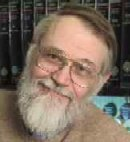
\includegraphics[width=3.44cm,height=3.969cm]{./img/kernighan.jpg} 
 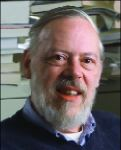
\includegraphics[width=3.44cm,height=3.969cm]{./img/dennis_ritchie.jpg} 
 \caption{Brian Kernighan y Dennis Ritchie, los creadores del lenguaje C} 
 \label{fig:kandr} 
 \end{figure} 


Algunas nuevas características de C99 son: 

\begin{itemize}
\item Matrices de tamaño variable 
\item Soporte de números complejos 
\item Tipos \code{long long int} y \code{unsigned long long int} de al menos 64 bits 
\item Familia de funciones \code{vscanf()} 
\item Comentarios al estilo de C++ prefijando las líneas con la secuencia \code{//}. 
\item Familia de funciones \code{snprintf()} 
\item Tipo boolean
\end{itemize}

%TODO C11

\section{El ciclo de compilación}
Las herramientas esenciales de un ambiente de desarrollo, además de
cualquier \textbf{editor de textos}, son el \textbf{compilador}, el \textbf{vinculador}, 
\textbf{linkeditor} o \textit{linker}, y el \textbf{bibliotecario}. A
estas herramientas básicas se agregan otras, útiles para
automatizar la compilación de proyectos extensos, almacenar y
recuperar versiones de programas fuente, comprobar sintaxis en forma
previa a la compilación, etc. Según el ambiente operativo y
producto de software de que se trate, estas herramientas pueden ser comandos de línea independientes, con
salidas de texto simples, o encontrarse integradas en una interfaz de usuario uniforme, en modo
texto o modo gráfico. 

Cuando encontramos varias de estas herramientas integradas en una sola aplicación, decimos que se trata de un \textbf{IDE} (\textit{Integrated Development Environment}) o ambiente de desarrollo integrado. Un IDE oculta el ciclo de compilación al usuario, con la intención de simplificar el proceso de desarrollo. Sin embargo, conviene conocer qué función se cumple, y qué producto se espera, en cada fase del ciclo de compilación, para poder interpretar las diferentes situaciones de error y poder corregirlas.

\figura[12]{ciclo}{El ciclo de compilación produce un ejecutable a partir de archivos fuente.}{ciclo.eps}

\subsection{Compilador}
\begin{itemize}
	\item El compilador acepta un archivo \textbf{fuente}, posiblemente relacionado con
otros (una \textbf{unidad de traducción}), y genera con él un
\textbf{módulo objeto}. Este módulo objeto contiene porciones de
código ejecutable mezclado con \textbf{referencias}, aún no resueltas, a
variables o funciones cuya definición no figura en los fuentes de
entrada. Estas referencias quedan en forma simbólica en el módulo
objeto hasta que se resuelvan en un paso posterior. 
\item Si ocurren errores en esta fase, se deberán a problemas de sintaxis (el código escrito por el programador no respeta la definición del lenguaje).
\end{itemize}

\subsection{Vinculador, linkeditor o \textit{linker}}
\begin{itemize}
\item El vinculador recibe como entrada un conjunto de módulos objeto y
busca \textbf{resolver}, vincular, o enlazar, las referencias simbólicas en ellos,
buscando la definición de las variables o funciones faltantes en los
mismos objetos o en bibliotecas. Éstas pueden ser la Biblioteca
Standard, u otras provistas por el usuario. Cuando el linker encuentra la
definición de un objeto buscado (es decir, de una variable o
función), la copia en el archivo resultante de salida (la
\textit{resuelve}). El objetivo del linker es resolver todas las
referencias pendientes para producir un programa ejecutable. 
\item Si ocurren errores en esta fase, se deberán a que existen variables o funciones cuya definición no ha sido dada (no se encuentran en las unidades de traducción procesadas, ni en ninguna biblioteca conocida por el linker).
\end{itemize}

\subsection{Bibliotecario}
\begin{itemize}
	\item El bibliotecario es un programa administrador de módulos objeto. Su función
es reunir módulos objeto en archivos llamados \textbf{bibliotecas}, y luego
permitir la extracción, borrado, reemplazo y agregado de módulos.
El conjunto de módulos en una biblioteca se completa con una tabla de
información sobre sus contenidos para que el linker pueda encontrar
rápidamente aquellos módulos donde se ha definido una variable o
función, y así extraerlos durante el proceso de linkedición. 
\item El bibliotecario es utilizado por el usuario cuando desea mantener sus
propias bibliotecas. La creación de bibliotecas propias del usuario
ahorra tiempo de compilación y permite la distribución de software
sin revelar la forma en que se han escrito los fuentes y
protegiéndolo de modificaciones. 
\end{itemize}

Una vez que el código ha sido compilado y vinculado, obtenemos un programa ejecutable. Los errores que pueden producirse en la ejecución ya no corresponden a problemas de compilación, sino que se deben a aspectos de diseño del programa que deben ser corregidos por el programador.

\section{Un primer ejemplo}

El clásico ejemplo de todas las introducciones al lenguaje C es un programa llamado \quotes{\textbf{Hello, World!}}.

\begin{lstlisting}
#include <stdio.h>

/* El primer programa! */
int main()
{
	printf("Hola, gente!\n");
}
\end{lstlisting}

\subsection{Estructura del programa}

\begin{itemize}
\item Este programa minimal comienza con una \textbf{directiva de preprocesador} que indica incluir en la unidad de traducción al
archivo de cabecera o \textit{header} \textbf{stdio.h}. Éste contiene, entre otras
cosas, la declaración (o \textbf{prototipo}) de la función de
salida de caracteres \textbf{printf()}, perteneciente a la Biblioteca Standard. Los prototipos se incluyen para
advertir al compilador de los tipos de las funciones y de sus
argumentos. 
\item Entre los pares de caracteres especiales \textbf{/*} y \textbf{*/}se puede insertar cualquier cantidad de líneas de comentarios. 
\item La función \textbf{main()} es el cuerpo principal del programa
(es por donde comenzará la ejecución). Todas las funciones en C están delimitadas por un par de llaves. Terminada la ejecución de
main(), terminará el programa. 
\item La función \code{printf()} imprimirá la cadena entre comillas, que es
una \textbf{constante string} terminada por un carácter de
\textbf{nueva línea} (la secuencia especial \quotes{\code{\\n}}). 
\end{itemize}

\subsection{Compilación del programa}
Para ver el primer ejemplo en C en funcionamiento:

\begin{enumerate}
	\item Copiar el programa con cualquier editor de textos y guardarlo en un archivo llamado \code{hola.c} en el directorio de trabajo del usuario.
	\item Sin cambiar de directorio, invocar al compilador ejecutando el comando \code{gcc hola.c -o hola}. Por defecto, el compilador \textbf{gcc} invocará al vinculador \textbf{ld} para generar el ejecutable a partir del archivo objeto intermedio generado. 
	\item Ejecutar el programa con el comando \code{./hola}. 
\end{enumerate}

Notar el \textit{punto y barra} del principio al ejecutar el programa. El punto y barra le indican al \textbf{shell} que debe buscar el programa en el directorio activo.

\subsubsection{Otra manera} 
%Lo mismo, pero de otra manera:
\begin{enumerate}
	\item Como antes, copiar el programa, o usar el mismo archivo fuente de hace un momento.
	\item Sin cambiar de directorio, ejecutar el comando \code{make hola} en una consola o terminal.
	\item Ejecutar el programa con el comando \code{./hola}. 
\end{enumerate}

La diferencia es que en el primer caso invocamos directamente al compilador \code{gcc},
mientras que en el segundo caso utilizamos la herramienta \code{make}, que nos asiste en la compilación de proyectos. En el ejemplo, le decimos al compilador que procese el archivo fuente \code{hola.c}, y que el ejecutable de salida (opción \code{-o}, de \textit{output}) reciba el nombre \code{hola}. 


% \subsection[Mapa de memoria de un programa Mas información ... ]{Mapa de memoria de un programa \href{info/info1.html#info2}{Mas información ...} }

\subsection{El comando make}
Cuando damos un comando como \code{make hola}, utilizamos el comando \textbf{make} para compilar y vincular el programa \textbf{hola.c}. El comando \textbf{make} contiene la inteligencia para:
\begin{itemize}
 	\item buscar, en el directorio activo, archivos fuente llamados \textbf{hola.*}; 
 	\item determinar (a partir de la extensión) que el hallado se trata de un programa en C;
 	\item ver que no existe en el directorio activo un programa ejecutable llamado \textbf{hola}, o que, si existe, su fecha de última modificación es anterior a la del fuente;
 	\item razonar que, por lo tanto, es necesario compilar el fuente \textbf{hola.c} para producir el ejecutable \textbf{hola};  
 	\item e invocar con una cantidad de opciones por defecto al compilador \textbf{gcc}, y renombrar la salida con el nombre
\textbf{hola}. Éste será el ejecutable que deseamos producir.
\end{itemize} 

Si se invoca al comando \textbf{make} una segunda vez, éste comprobará, en base a las fechas de
modificación de los archivos fuente y ejecutable, que no es necesaria la compilación (ya que el
ejecutable es posterior al fuente). Si editamos el fuente para cambiar algo en el programa, invocar
nuevamente a \textbf{make} ahora repetirá la compilación (porque ahora el fuente es posterior al ejecutable).


\subsubsection{Makefiles}
En casos sencillos, el comando \textbf{make} puede hacer en forma autónoma todo el trabajo descripto anteriormente. Sin embargo, cuando se construyen proyectos más complejos, formados por muchos fuentes con interdependencias complejas, o cuando se requieren diferentes opciones del proceso de compilación (o aun diferentes compiladores), entonces es conveniente escribir una guía de actividades para \textbf{make}. Esta guía se guarda en un archivo llamado \textbf{makefile} o \textbf{Makefile}. Al ser invocado, el programa \textbf{make} buscará un archivo con alguno de esos nombres en el directorio actual, y si lo encuentra, ejecutará las tareas que se indican allí.  

Un \textbf{makefile} tiene una sintaxis específica y sumamente compleja, pero suele ser suficiente con conocer unas pocas reglas de escritura para escribir \textbf{makefiles} que resulten útiles. 

\begin{itemize}
	\item Los objetos que se desea construir se llaman \textbf{goals} o metas. Se indican con rótulos al principio del renglón y seguidos por dos puntos.
	\item Las dependencias de cada \textbf{goal} se escriben inmediatamente después de los dos puntos. Las dependencias son los archivos cuya fecha \textbf{make} comprobará para saber si debe reconstruir un \textbf{goal} o no.
	\item Las acciones que se debe llevar a cabo para cada \textbf{goal}, en caso de que deba ser reconstruido, se indican a continuación, sin renglones intermedios, e indentadas.
	\item Un \textbf{goal}, sus dependencias y las acciones asociadas, se separan de las demás con un renglón en blanco.
\end{itemize}

Así, por ejemplo, el siguiente \textbf{makefile} es equivalente al conocimiento que \textbf{make} aplicó para construir el programa de nuestro primer ejemplo:

\begin{lstlisting}
hola: hola.c
	gcc hola.c -o hola
	
\end{lstlisting}

Se recomienda consultar el manual del comando \textbf{make}, ya que es muy útil para el desarrollador C dominar el lenguaje de escritura de \textbf{makefiles}. En particular, es valioso comprender que \textbf{make} es versátil y puede utilizarse para automatizar muchas otras tareas, no solamente las de desarrollo de programas.


\section{Mapa de memoria de un programa}
Luego de la compilación y vinculación, el programa ejecutable queda contenido en un archivo. Al ser invocado, el sistema operativo lo carga en memoria, y allí se despliega en una cantidad de secciones de diferentes tamaños y con distintas funciones. 

Los sistemas operativos modernos, salvo raras excepciones, administran la memoria física  usando sistemas de memoria virtual. Cada sistema de memoria virtual funciona de modo diferente. La manera como se distribuyen realmente las secciones de un programa en la memoria física depende fuertemente de la
forma de administración de memoria del sistema operativo para el cual ha sido compilado y vinculado. Sin embargo,
el siguiente modelo puede servir de referencia para ilustrar algunas particularidades y problemas
que irán surgiendo con el estudio del lenguaje.

El programa cargado en memoria (Fig. \ref{fig:mapa}) se dividirá en cuatro regiones: código o \textbf{texto}, \textbf{datos
estáticos}, \textbf{heap} (o región de datos dinámicos), y \textbf{stack} (o pila). 

El tamaño de las regiones de código y de datos estáticos está determinado al momento de compilación
y es inamovible. Las otras dos regiones quedan en un bloque cuyo tamaño inicial es ajustado por el
sistema operativo al momento de la carga, pero puede variar durante la ejecución. Este bloque es
compartido entre ambas regiones. Una de ellas, la de datos dinámicos, o heap, crece \quotes{hacia arriba} (hacia 
direcciones de memoria más altas); la otra, la pila del programa, o stack, crece \quotes{hacia abajo} (en
sentido opuesto).


\figura[4]{mapa}{El mapa de memoria de un programa se divide conceptualmente en cuatro regiones.}{mapadememoria.eps}

\begin{description}
	\item[Texto del programa] La región de texto contendrá el \textbf{código del programa}, es decir, la versión ejecutable de las
\textbf{instrucciones} que escribió el programador, traducidas por el compilador al lenguaje de la máquina. En
general, el programa fuente C se compondrá de funciones, que serán replicadas a nivel de máquina por
subrutinas en el lenguaje del procesador subyacente. Algunas instrucciones C resultarán en última
instancia en invocaciones a funciones del sistema (por ejemplo, cuando necesitamos escribir en un
archivo).
	\item[Datos estáticos] La región de datos estáticos es un lugar de almacenamiento para datos del programa que quedan
definidos al momento de la compilación. Se trata de datos cuya vida o instanciación no depende de la
invocación de las funciones. Son las variables estáticas, definidas en el cuerpo del programa que es
común a todas las funciones. A su vez, esta zona se divide en dos: la de \textbf{datos estáticos inicializados}
explícitamente por el programa (zona a veces llamada \textbf{bss} por motivos históricos) y la zona de \textbf{datos
estáticos sin inicializar} (a veces llamada \textbf{data}), que será llenada con ceros binarios al momento de la
carga del programa.
	\item[Stack] El stack, o \textbf{pila}, aloja las variables locales de las funciones a medida que esas funciones son invocadas. Cada función que declare variables locales obtendrá espacio de almacenamiento para esas variables en el stack. Al terminar la función, como el ámbito de sus variables desaparece, esas variables son desalojadas, y el espacio que ocupaban vuelve a quedar disponible. 
	\item[Heap] Un programa C puede utilizar estructuras de datos dinámicas, como listas o árboles, que vayan
creciendo al agregárseles elementos. El programa puede \quotes{pedir} memoria cada vez que necesite alojar
un nuevo elemento de estas estructuras dinámicas, o para crear buffers temporarios para cualquier uso
que sea necesario. El \textbf{heap} es la zona de donde el programa obtiene esos trozos de memoria, solicitada en forma dinámica al sistema operativo. El límite del heap se irá desplazando hacia las direcciones superiores.

\end{description}

\importante{
A diferencia de otros lenguajes con administración de memoria automática, en C normalmente es necesario solicitar en forma explícita cada segmento de memoria asignada dinámicamente. Es responsabilidad del programador, también, liberar esta memoria cuando no ya sea necesaria, ya que en C no existe un
mecanismo de \quotes{recolección de basura}, lo cual sí existe en otros lenguajes, para desalojar
automáticamente objetos que ya no se utilicen.\\


Por otro lado, un programa que realice una cadena de invocaciones de muchas funciones, 
especialmente si éstas utilizan muchas variables locales (y aún más especialmente si el programa es recursivo), hará crecer notablemente su stack,
desplazando el tope de la pila hacia abajo. La destrucción de las variables locales sí es automática, y se produce al momento de finalizar la ejecución de la función.
}

% La región del stack es el lugar para la creación y destrucción de variables locales, que son aquellas que viven mientras tiene lugar la ejecución de la función a la que pertenecen. 

Este modelo será útil en varias ocasiones para explicar algunas cuestiones especiales del lenguaje C.

%TODO http://www.ualberta.ca/CNS/RESEARCH/LinuxClusters/mem.html

\begin{ejemplo}
Analicemos en qué lugares quedarán alojados los elementos del programa siguiente.
\begin{lstlisting}
int a = 1;
int b;

int fun()
{
	int c;
	c = a + b;
}

int main()
{
	fun();
}
\end{lstlisting} 

\begin{itemize}
	\item Las variables \code{a} y \code{b} corresponden a la zona de datos estáticos. La variable \code{a} está inicializada con 1, pero como \code{b} no está inicializada, recibirá un valor 0.
\item La variable \code{c} aparecerá en el stack cuando se ejecute la función \code{fun()}.
\item Las instrucciones de máquina procedentes de la compilación del programa (funciones \code{main()} y \code{fun()}) serán almacenadas en la región de texto. 

\end{itemize}
\end{ejemplo}






\begin{preguntas}
\label{sec:tc-introduccion-preg}
\question El principal objetivo de diseño de quienes crearon el C era
\choice Posibilidad de acceder a los recursos de hardware.
\choice Portabilidad del compilador.
\choice Eficiencia del código generado.
\correctchoice Todas las anteriores.

\question La primera definición oficial del lenguaje fue dada por Kernighan y Ritchie en
\choice 1975.
\correctchoice 1978.
\choice 1983.
\choice 1988.

\question Las palabras reservadas de C son
\choice Muchas.
\correctchoice Pocas.
\choice Exactamente las de entrada/salida.
\choice Exactamente tantas como las de Pascal.

\question La Biblioteca Standard de C
\choice Provee funciones para todas las necesidades.
\choice Está escrita por el usuario.
\correctchoice No provee funciones para todas las necesidades.

\question El lenguaje C
\choice No realiza recolección de basura pero sí controles de tiempo de ejecución.
\choice No realiza controles de tiempo de ejecución pero sí recolección de basura.
\choice Realiza ambas cosas.
\correctchoice Ninguna de las dos cosas.

\question Los programas en C son portables porque
\choice Se lo dotó de control de tipos de datos.
\correctchoice Los tipos de datos no tienen un tamaño definido por el lenguaje.
\choice Los tamaños de los tipos de datos son idénticos en todas las implementaciones.
\choice Se lo basó en una única arquitectura.

\question El pasaje de argumentos a funciones en C se hace
\correctchoice por valor.
\choice por referencia.
\choice por nombre.

\question El lenguaje C pertenece al paradigma
\choice Lógico.
\correctchoice Procedural.
\choice Funcional.
\choice Orientado a objetos.

\question Las herramientas del ciclo de compilación comprenden
\choice compilador y linkeditor.
\correctchoice editor, compilador, linkeditor y bibliotecario.
\choice compilador y Biblioteca Standard.

\question El utilitario \code{make} genera
\choice archivos objeto.
\choice ejecutables.
\choice bibliotecas.
\correctchoice todo lo anterior.

\question El mapa de memoria del programa comprende
\choice Dos regiones estáticas y dos dinámicas.
\choice Cuatro regiones en total.
\choice Regiones de texto, de datos estáticos, de heap y de stack .
\correctchoice Todo lo anterior.

\question La región de pila almacena
\correctchoice las variables locales.
\choice las variables estáticas.
\choice las estructuras de datos dinámicas.
\choice el código del programa.
\end{preguntas}

\section{Ejercicios}
\label{sec:tc-introduccion-ej}
\begin{enumerate}
	\item ¿Qué nombres son adecuados para los archivos fuente C? 
	\item Describa las etapas del ciclo de compilación.
	\item ¿Cuál sería el resultado de: 
		\begin{itemize}
		\item Editar un archivo fuente? 
		\item Ejecutar un archivo fuente? 
		\item Editar un archivo objeto? 
		\item Compilar un archivo objeto? 
		\item Editar una biblioteca?
		\end{itemize}
	\item ¿Qué pasaría si un programa en C \textbf{no} contuviera una función \code{main()}? Haga la prueba modificando \textbf{hola.c}.
	\item Edite el programa \textbf{hola.c} y modifíquelo según las pautas que siguen. Interprete los errores de compilación. Identifique en qué etapa del ciclo de compilación ocurren los errores. Si resulta un programa ejecutable, observe qué hace el programa y por qué. 
		\begin{itemize}
		\item Quite los paréntesis de \code{main()}. 
		\item Quite la llave izquierda de \code{main()}.
		\item Quite las comillas izquierdas.
		\item Quite los caracteres \quotes{\code{\\n}}.
		\item Agregue al final de la cadena los caracteres \quotes{\code{\\n\\n\\n\\n}}.
		\item Agregue al final de la cadena los caracteres \quotes{\code{\\nAdiós, mundo!\\n}}.
		\item Quite las comillas derechas.
		\item Quite el signo punto y coma. 
		\item Quite la llave derecha de \code{main()}.
		\item Agregue un punto y coma en cualquier lugar del texto.
		\item Agregue una coma o un dígito en cualquier lugar del texto. 
		\item Reemplace la palabra \code{main} por \code{program}, manteniendo los paréntesis. 
		\item Elimine la apertura o cierre de los comentarios.
		\end{itemize}
\end{enumerate}



\chapter{El preprocesador}
\label{chap:tc-preprocesador}

El compilador C tiene un componente auxiliar llamado \textbf{preprocesador}, que actúa en la primera etapa del proceso de compilación. Su misión es buscar, en el texto del programa fuente entregado al compilador, ciertas \textbf{directivas} que le indican realizar alguna tarea a nivel de texto. Por ejemplo, \textbf{inclusión} de otros archivos, o \textbf{sustitución} de ciertas cadenas de caracteres (\textbf{símbolos} o \textbf{macros}) por otras. 

El preprocesador cumple estas directivas en forma similar a como podrían ser hechas interactivamente por el usuario, utilizando los comandos de un editor de texto (\quotes{incluir archivo} o \quotes{reemplazar texto}), pero en forma automática. Una vez cumplidas todas estas directivas, el preprocesador entrega el texto resultante al resto de las etapas de compilación, que terminarán dando por resultado un módulo objeto. Un archivo fuente, junto con todos los archivos que incluya, es llamado una \textbf{unidad de traducción}.

\figura[12]{preproc1}{El preprocesador realiza ediciones automáticas de los fuentes.}{ciclo-wmf.eps}

El preprocesador sirve para eliminar redundancia y aumentar la expresividad de los programas en C, facilitando su mantenimiento. Si una variable o función se utiliza en varios archivos fuente, es posible aislar su declaración, colocándola en un único archivo aparte que será incluido al tiempo de compilación en los demás fuentes. Esto facilita toda modificación de elementos comunes en los fuentes de un proyecto. Por otro lado, si una misma constante o expresión aparece repetidas veces en un texto, y es posible que su valor deba cambiarse más adelante, es muy conveniente definir esa constante con un símbolo y especificar su valor sólo una vez, mediante un símbolo o macro.

\section{Directivas de preprocesador}

Las directivas del preprocesador no pertenecen al lenguaje C en un sentido estricto. El preprocesador \textbf{no comprende ningún aspecto sintáctico ni semántico} de C. Las \textbf{macros} definidas en un programa C \textbf{no son variables ni funciones}, sino simplemente cadenas de texto que el preprocesador deberá sustituir por otras. Las directivas pueden aparecer en cualquier lugar del programa, pero sus efectos se ponen en vigor recién a partir del punto del programa en que aparecen, y hasta el final de la unidad de traducción. Es decir, un símbolo o macro puede utilizarse sólo después de la aparición de la directiva que la define, y no antes. Tampoco puede utilizarse en una unidad de traducción diferente, salvo que vuelva a ser definida en ella (los símbolos de preprocesador no se \quotes{propagan} entre unidades de traducción).

\subsection{Símbolos y macros}
Una de las funciones del preprocesador es sustituir símbolos, o cadenas de texto dadas, por otras 
(Fig. \ref{fig:preproc1}). La directiva \lstinline{define} establece la relación entre los símbolos y su \textbf{expansión}, o cadena 
a sustituir. Los símbolos indicados con una directiva de definición \lstinline{define} se guardan en una \textbf{tabla de símbolos} durante el preprocesamiento. 

Habitualmente se llama \textbf{símbolos} a aquellas cadenas que son directamente sustituibles por una expresión, reservándose el nombre de \textbf{macros} para aquellos símbolos cuya expansión es parametrizable (es decir, llevan argumentos formales y reales como en el caso de las funciones). La cadena de expansión puede ser cualquiera, no necesariamente un elemento sintácticamente válido de C.

\figura[10]{direct}{Transformaciones realizadas por directivas de preprocesador.}{directivas.eps}

\begin{ejemplo}
La Fig. \ref{fig:direct} muestra el programa ejemplo \textbf{hola.c} escrito usando directivas de inclusión de archivos, símbolos y macros, y las sucesivas transformaciones que hará el preprocesador. 

El texto del programa una vez preprocesado quedará idéntico al del programa \textbf{hola.c} anteriormente presentado, y listo para ingresar a la etapa de compilación propiamente dicha. 
\end{ejemplo}

\nota{
\begin{enumerate}
	\item 
\begin{lstlisting}
#include <stdio.h>

#define MENSAJE "Hola, gente!\n"
#define IMPRIMIR(x) printf(x)

int main()
{
	IMPRIMIR(MENSAJE);
}
\end{lstlisting}

\item
\begin{lstlisting}
... declaraciones en stdio.h ...
#define MENSAJE "Hola, gente!\n"
#define IMPRIMIR(x) printf(x)
int main()
{
	IMPRIMIR(MENSAJE);
}
\end{lstlisting}

\item
\begin{lstlisting}
... declaraciones en stdio.h ...
#define IMPRIMIR(x)	printf(x)

int main()
{
	IMPRIMIR("Hola, gente!\n");
}
\end{lstlisting}

\item
\begin{lstlisting}
... declaraciones en stdio.h ...

int main()
{
	printf("Hola, gente!\n");
}
\end{lstlisting}

\end{enumerate}
}

\subsection{Headers}
Las directivas para incluir archivos suelen darse al principio de los programas, ya que en general se desea que su efecto alcance a todo el archivo fuente. Por esta razón los archivos preparados para ser incluidos se denominan \textit{headers} o archivos de cabecera. La implementación de la Biblioteca Standard que viene con un compilador posee sus propios headers, uno por cada módulo de la biblioteca, que \textbf{declaran} funciones y variables de uso general. Estos headers contienen texto legible por humanos, y están en algún subdirectorio predeterminado (llamado \lstinline{/usr/include} en UNIX, y dependiendo del compilador en otros sistemas operativos). El usuario puede escribir sus propios headers, y no necesita ubicarlos en el directorio reservado del compilador; puede almacenarlos en el directorio activo durante la compilación. 

En el párrafo anterior, nótese que decimos \textbf{declarar} funciones, y no \textbf{definirlas}; la diferencia es importante y se verá en profundidad más adelante. Recordemos por el momento que \textbf{en los headers} de la Biblioteca Standard no aparecen \textbf{definiciones} -es decir, textos- de funciones, sino solamente \textbf{declaraciones o prototipos}, que sirven para anunciar al compilador detalles como los tipos y cantidad de los argumentos de las funciones.

No se considera buena práctica de programación colocar la definición de una función de uso frecuente en un header. Esto obligaría a recompilar siempre la función cada vez que se la utilizara. Por el contrario, lo ideal sería compilarla una única vez, produciendo un módulo objeto (y posiblemente incorporándolo a una biblioteca). Esto ahorraría el tiempo correspondiente a su compilación, ocupando
sólo el necesario para la vinculación.

% La directiva \lstinline{\#include} hace que el preprocesador inserte y preprocese otros archivos en el punto donde se indica la directiva. El resultado de preprocesar el archivo incluido puede ser definir otros símbolos y macros, o aun incluir otros archivos. Los archivos destinados a ser incluidos son habitualmente llamados archivos de cabecera o headers. Las directivas de inclusión son anidables, es decir, pueden incluirse headers que a su vez contengan directivas de inclusión. 

\section{Definición de símbolos}

Si el programa dice:
\begin{lstlisting}
a = 2 * 3.14159 * 20.299322;
\end{lstlisting}
Es mucho más claro poner, en su lugar:
\begin{lstlisting}
#define PI	3.14159
#define RADIO	20.299322

a = 2 * PI * RADIO;
\end{lstlisting}



\section{Definición de macros}
Con las siguientes directivas:
\begin{lstlisting}
#include <stdio.h>
#include "aux.h"
#define MAXITEM 100
#define DOBLE(X) 2*X
\end{lstlisting}

\begin{itemize}
	\item Se incluye el header de Biblioteca Standard \lstinline{stdio.h}, que contiene declaraciones necesarias para
poder utilizar funciones de entrada/salida standard (hacia consola y hacia archivos).
\item Se incluye un header \lstinline{aux.h} escrito por el usuario. Al indicar el nombre del header entre ángulos, como en la línea anterior, especificamos que la búsqueda debe hacerse en los directorios reservados del compilador. Al indicarlo entre comillas, nos referimos al directorio actual.
\item Se define un símbolo MAXITEM equivalente a la constante numérica 100.
\item Se define una macro DOBLE(X) que deberá sustituirse por la cadena 2*(argumento de la llamada
a la macro).
\end{itemize}

De esta manera, podemos escribir sentencias tales como:
\begin{lstlisting}
a=MAXITEM;
b=DOBLE(45);
\end{lstlisting}
El texto luego de la etapa de preprocesamiento y antes de la compilación propiamente dicha será
\begin{lstlisting}
a=100;
b=2*45;
\end{lstlisting}

\subsection{Macros vs. funciones}
Es importante comprender que, aunque sintácticamente parecido, el uso de una macro \textbf{no es una
llamada a función}; los argumentos de una macro no se evalúan en tiempo de ejecución antes de la
llamada, sino que \textbf{se sustituyen textualmente} en el cuerpo de la macro. Así, si ponemos
\begin{lstlisting}
#define DOBLE(X) 2*X
b=DOBLE(40+5);
\end{lstlisting}
el resultado será \lstinline{b=2*40+5}; y no \lstinline{b=2*45}, ni \lstinline{b=2*(40+5)}, que presumiblemente es lo que desea el
programador.

Este problema puede solucionarse redefiniendo la macro así:
\begin{lstlisting}
#define DOBLE(X) 2*(X)
b=DOBLE(40+5);
\end{lstlisting}
Ahora la expansión de la macro será la deseada. En general, es saludable rodear las apariciones de los
argumentos de las macros entre paréntesis, para obligar a su evaluación al tiempo de ejecución con la
precedencia debida, y evitar efectos laterales.


\section{Compilación condicional}

Una característica interesante del preprocesador es que permite la \textbf{compilación condicional} de segmentos de la unidad de traducción, en base a valores de símbolos. Una directiva condicional es aquella que comprueba si un símbolo dado ha sido definido, o si su definición coincide con cierta cadena. El texto del programa que figura entre la directiva y su \lstinline{end} será considerado sólo si la comprobación resulta exitosa. Los símbolos o macros pueden ser definidos al tiempo de la compilación, sin alterar el texto del programa, permitiendo así una parametrización del programa en forma separada de su escritura.

\begin{ejemplo}
Con las directivas condicionales:
\begin{itemize}
	\item Definimos una macro \lstinline{CARTEL} que equivaldrá a invocar a una función \quotes{imprimir},
pero sólo si el símbolo \lstinline{DEBUG} ha sido definido. En otro caso, equivaldrá a la cadena vacía. 
\begin{lstlisting}
#ifdef DEBUG
#define CARTEL(x)	imprimir(x)
#else
#define CARTEL(x)
#endif
\end{lstlisting}
\item El segmento siguiente muestra un caso con lógica inversa pero equivalente al ejemplo anterior.
\begin{lstlisting}
#ifndef DEBUG
#define CARTEL(x)
#else
#define CARTEL(x) imprimir(x)
#endif
\end{lstlisting}
\item En el caso siguiente, se incluirá uno u otro header dependiendo del valor del símbolo \lstinline{SISTEMA}. Tanto
\lstinline{DEBUG} como \lstinline{SISTEMA} pueden tomar valores al momento de compilación, si se dan como
argumentos para el compilador. De esta manera se puede modificar el comportamiento del programa
sin necesidad de editarlo.

\begin{lstlisting}
#if SISTEMA==MS_DOS
#include "header1.h"
#elif SISTEMA==UNIX
#include "header2.h"
#endif
\end{lstlisting}
\end{itemize}
\end{ejemplo}

\section{Observaciones}
\begin{itemize}
	\item A veces puede resultar interesante, para depurar un programa, observar cómo queda el archivo
intermedio generado por el preprocesador después de todas las sustituciones, inclusiones, etc. La
mayoría de los compiladores cuentan con una opción que permite generar este archivo intermedio y
detener allí la compilación, para poder estudiarlo.
	\item Otra opción relacionada con el preprocesador que suelen ofrecer los compiladores es aquella que
permite definir, al tiempo de la compilación y sin modificar los fuentes, símbolos que se pondrán a la
vista del preprocesador. Así, la estructura final de un programa puede depender de decisiones tomadas
al tiempo de compilación. Esto permite, por ejemplo, aumentar la portabilidad de los programas, o
generar múltiples versiones de un sistema sin diseminar el conocimiento reunido en los módulos
fuente que lo componen.
	\item Finalmente, aunque el compilador tiene un directorio default donde buscar los archivos de inclusión,
es posible agregar otros directorios para cada compilación con argumentos especiales si es necesario.
\end{itemize}



\begin{preguntas}
\label{sec:tc-preprocesador-preg}
\question El preprocesador interviene
\choice Después de la compilación del código.
\correctchoice Antes de la compilación del código.

\question El preprocesador promueve
\correctchoice La legibilidad.
\choice La redundancia.
\choice La rapidez de ejecución.
\choice Todas las anteriores.

\question El preprocesador facilita
\choice El mantenimiento.
\choice La legibilidad.
\choice La expresividad.
\correctchoice Todas las anteriores.

\question Las directivas de preprocesador
\choice Están contenidas en el lenguaje C.
\choice Son variables de texto.
\correctchoice No pertenecen al lenguaje C.
\choice Son palabras reservadas.
\choice Son funciones de C.

\question El efecto de las directivas de preprocesador abarca
\choice La función donde están declaradas.
\correctchoice La unidad de traducción.
\choice El proyecto de programación.
\choice El bloque donde están declaradas.

\question Los headers
\choice Son escritos por el usuario.
\choice Vienen con el compilador.
\correctchoice Todas las anteriores.
\choice Ninguna de las anteriores.

\question Los headers que \textbf{definen} funciones
\choice son recomendables.
\choice son imprescindibles.
\correctchoice no son recomendables.
\choice son recomendables pero no imprescindibles.

\question ¿Cuál es la directiva de preprocesador correcta si queremos definir un símbolo ALFA con valor 1?
\choice \code{#ALFA = 1}
\choice \code{#define ALFA = 1}
\correctchoice \code{#define ALFA 1}
\choice \code{#define 1 ALFA}

\question ¿Cuál es la directiva de preprocesador correcta si queremos incluir el header de Biblioteca Standard \code{stdio.h}?
\choice \code{#include stdio.h}
\choice \code{#include <stdio>}
\correctchoice \code{#include <stdio.h>}
\choice Cualquiera de las anteriores.

\question La directiva correcta para crear una macro que devuelva el doble de su argumento es
\choice \code{#DOBLE(x) 2*x}
\choice \code{#define DOBLE 2*x}
\correctchoice \code{#define DOBLE(x) 2*(x)}
\choice \code{#define DOBLE(x) 2*(x);}
\choice \code{#define DOBLE(x) 2 * (x)}

\question ¿Cuál es la directiva correcta para incluir un header llamado  \code{beta.h} situado en el directorio donde se está realizando la compilación?
\choice \code{#define <beta.h>}
\choice \code{#include <beta.h>}
\correctchoice \code{#include "beta.h"}

\question Normalmente los headers contienen
\correctchoice Declaraciones de variables y funciones.
\choice Definiciones de variables y funciones.
\choice Prototipos de directivas.
\choice Inclusión de archivos fuente.
\choice Todas las anteriores.

\question Las directivas condicionales consideran un segmento de texto
\choice sólo si la compilación resulta exitosa.
\correctchoice sólo si la condición resulta exitosa.

\question El resultado de preprocesar la macro \code{#define FUNCION(x) 3*x+1} aplicada al argumento \code{2+1} será 
\choice \code{3*3+1}
\correctchoice \code{3*2+1+1}
\choice \code{7}
\choice \code{8}

\question El problema de la expansión errónea de las macros se soluciona 
\choice Rodeando los argumentos entre signos \code{\<\>}.
\choice Rodeando los argumentos con corchetes.
\choice Poniendo la macro completa entre comillas.
\correctchoice Rodeando los argumentos con paréntesis.
\end{preguntas}


\section{Ejercicios}
\label{sec:tc-preprocesador-ej}
\begin{enumerate}
	\item Dé ejemplos de directivas de preprocesador:
		\begin{enumerate}[label=\alph*.]
\item Para incluir un archivo proporcionado por el compilador.
\item Para incluir un archivo confeccionado por el usuario.
\item Para definir una constante numérica.
\item Para compilar un segmento de programa bajo la condición de estar definida una constante.
\item Idem bajo la condición de ser no definida.
\item Idem bajo la condición de que un símbolo valga una cierta constante.
\item Idem bajo la condición de que dos símbolos sean equivalentes.
\end{enumerate}
\item Proponga un método para incluir un conjunto de archivos en un módulo fuente con una sola
directiva de preprocesador.
 \item ¿Cuál es el ámbito de una definición de preprocesador? Si defino un símbolo A en un fuente y lo
compilo creando un módulo objeto algo.o, ¿puedo utilizar A desde otro fuente, sin declararlo, a
condición de linkeditarlo con algo.o?
\item ¿Qué pasa si defino dos veces el mismo símbolo en un mismo fuente?
\item Un cierto header A es incluido por otros headers B, C y D. El fuente E necesita incluir a B, C y D.
Proponga un método para poder hacerlo sin obligar al preprocesador a leer el header A más de una
vez.
\item Edite el programa hello.c del ejemplo del capítulo 1 reemplazando la cadena \lstinline{"Hola, mundo!\n"} por
un símbolo definido a nivel de preprocesador.
\item  Edite el programa hello.c incluyendo la compilación condicional de la instrucción de impresión
printf() sujeta a que esté definido un símbolo de preprocesador llamado IMPRIMIR. Compile y pruebe
a) sin definir el símbolo IMPRIMIR, b) definiéndolo con una directiva de preprocesador, c)
definiéndolo con una opción del compilador. ¿En qué casos es necesario recompilar el programa?
\item  Escriba una macro que imprima su argumento usando la función printf(). Aplíquela para reescribir
hello.c de modo que funcione igual que antes.
\item  ¿Cuál es el resultado de preprocesar las líneas que siguen? Es decir, ¿qué recibe exactamente el
compilador luego del preprocesado?
\begin{lstlisting}
#define ALFA 8
#define BETA 2*ALFA
#define PROMEDIO(x,y) (x+y)/2
a=ALFA*BETA;
b=5;
c=PROMEDIO(a,b);
\end{lstlisting}
\item  ¿Qué está mal en los ejemplos que siguen?
	\begin{enumerate}[label=\alph*.]

\item  
\begin{lstlisting}
#define PRECIO 27.5
PRECIO=27.7;
\end{lstlisting}

\item  
\begin{lstlisting}
#define 3.14 PI
\end{lstlisting}

\item  
\begin{lstlisting}
#define doble(x) 2*x;
alfa=doble(6)+5;
\end{lstlisting}
\end{enumerate}
\item Investigue la función de los símbolos predefinidos \lstinline{__STDC__}, \lstinline{__FILE__} y \lstinline{__LINE__}.
\end{enumerate}




\chapter{Tipos de datos y expresiones}
\label{chap:tc-tipos}
En general, las \textbf{expresiones} en C se construyen conectando, mediante \textbf{operadores}, diversos elementos, tales
como \textbf{identificadores} de variables, \textbf{constantes} e invocaciones de \textbf{funciones}. Cada uno de estos
elementos tiene un valor al tiempo de ejecución, y debe ocupar -al menos temporariamente, mientras se calcula el resultado de la expresión- un
lugar en memoria. Al evaluar cada expresión, el compilador crea, para alojar cada subexpresión de las
que la constituyen, \textbf{objetos de datos}, que pueden pensarse como espacio de memoria reservado temporariamente para
contener valores. Al completar el cálculo de la expresión, el resultado nuevamente debe ser alojado en un objeto de datos propio. Estos espacios de memoria son de diferentes \quotes{tamaños} (cantidades de bits) de
acuerdo al \textbf{tipo de dato} de la subexpresión.

Así, las expresiones y subexpresiones en C asumen siempre un \textbf{tipo de datos}: alguno de los tipos básicos del lenguaje, o
uno definido por el usuario. Una expresión, según las necesidades, puede convertirse de un tipo a otro.
El compilador hace esto a veces en forma \textbf{automática}. Otras veces, el programador fuerza una
\textbf{conversión de tipo} para producir un determinado resultado.

\section{Declaración de variables}

Los \textbf{tipos básicos} son:
\begin{itemize}
	\item \lstinline{char} (un elemento del tamaño de un byte)
	\item \lstinline{int} (un número entero con signo)
	\item \lstinline{long} (un entero largo)
	\item \lstinline{float} (un número en punto flotante)
	\item \lstinline{double} (un número en punto flotante, doble precisión)
\end{itemize}

Cuando declaramos una variable o forzamos una conversión de tipo, utilizamos una \textbf{especificación de
tipo}. Ejemplos de declaración de variables:

\begin{lstlisting}
char a;
int alfa,beta;
float x1,x2;
\end{lstlisting}

Los \textbf{tipos enteros} (\lstinline{char}, \lstinline{int} y \lstinline{long}) admiten los modificadores \lstinline{signed} (con signo) y \lstinline{unsigned} (sin signo). Un objeto de datos \textbf{unsigned} utiliza todos sus bits para representar magnitud; un \textbf{signed} utiliza un bit para signo, en representación complemento a dos.

El modificador \lstinline{signed} sirve sobre todo para explicitar el signo de los chars. El default para un \lstinline{int} es
signed; el default para \lstinline{char} puede ser signed o unsigned, dependiendo del compilador.

\begin{lstlisting}
unsigned int edad;
signed char beta;
\end{lstlisting}


Un int puede afectarse con el modificador \lstinline{short} (corto).

\begin{lstlisting}
short i;
unsigned short k;
\end{lstlisting}


Cuando en una declaración aparece sólo el modificador unsigned o short, y no el tipo, \textbf{se asume int}. El
tipo entero se supone el tipo básico manejable por el procesador, y es el tipo por omisión en varias
otras situaciones. Por ejemplo, cuando no se especifica el \textbf{tipo del valor devuelto} por una función.

El modificador long puede aplicarse también a double. El tipo resultante puede tener más 
precisión que los no modificados.

\begin{lstlisting}
long double pi;
\end{lstlisting}

\section{Tamaños de los objetos de datos}

El lenguaje C no define el tamaño de los objetos de datos de un tipo determinado. Es decir, un entero
puede ocupar 16 bits en una implementación del compilador, 32 en otra, o aun 64. Un \lstinline{long} puede tener, o no, más bits
que un \lstinline{int}. Un \lstinline{short} puede ser, o no, más corto que un \lstinline{int}. Según \textbf{K\&R}, lo único seguro es que "\textit{un \lstinline{short} no es mayor que un \lstinline{int}, que a su vez no es mayor que \lstinline{long}}".

Por supuesto, distintos tamaños en bits implican diferentes rangos de valores. Si deseamos \textbf{portar} un
programa, hecho bajo una implementación del compilador, a otra, no es posible asegurar a priori el
rango que tomará un tipo de datos. La fuente ideal para conocer los rangos de los diferentes tipos, en
una implementación determinada, es --además del manual del compilador-- el header \lstinline{limits.h} de la
Biblioteca Standard. Debe recordarse que cualquier suposición que hagamos sobre el rango o tamaño
de un objeto de datos afecta la portabilidad de un programa en C.

Las siguientes líneas son parte de un archivo \lstinline{limits.h} para una implementación en particular:

\begin{lstlisting}
/* Minimum and maximum values a 'signed short int' can hold. */
#define SHRT_MIN	(-32768)
#define SHRT_MAX	32767
/* Maximum value an 'unsigned short int' can hold. (Minimum is 0.) */
#define USHRT_MAX	65535
/* Minimum and maximum values a 'signed int' can hold. */
#define INT_MIN	(-INT_MAX - 1)
#define INT_MAX	2147483647
/* Maximum value an 'unsigned int' can hold. (Minimum is 0.) */
#ifdef __STDC__
#define UINT_MAX 	4294967295U
#else
#define UINT_MAX  	4294967295
#endif
/* Minimum and maximum values a 'signed long int' can hold. */
#ifdef __alpha__
#define LONG_MAX 	9223372036854775807L
#else
#define LONG_MAX	2147483647L
#endif
#define LONG_MIN 	(-LONG_MAX - 1L)
/* Maximum value an 'unsigned long int' can hold. (Minimum is 0.) */
# ifdef __alpha__
#define ULONG_MAX	18446744073709551615UL
#else
#ifdef __STDC__
#define ULONG_MAX 	4294967295UL
#else
#define ULONG_MAX 4294967295L
#endif
#endif
\end{lstlisting}

Cuando una operación sobre una variable provoca overflow, no se obtiene ninguna indicación de error.
El valor sufre \textbf{truncamiento} a la cantidad de bits que pueda alojar la variable.

Así, en una implementación donde los ints son de 16 bits, si tenemos en una variable entera el máximo
valor positivo:

\begin{lstlisting}
int a; 
a=32767; /* a=0111111111111111 binario */
a=a+1;
\end{lstlisting}

Al calcular el nuevo valor de \lstinline{a}, aparece un 1 en el bit más significativo, lo cual, según la representación de los enteros, lo transforma en un negativo (el menor negativo que soporta el tipo de datos, -32768).

Si el int es sin signo:

\begin{lstlisting}
unsigned a;
a=65535; /* máximo valor de unsigned int */
a=a+1; 
\end{lstlisting}

el incremento de \lstinline{a} provoca overflow, y el nuevo valor de \lstinline{a} se trunca a 16 bits, volviendo así a 0.

Siempre se puede saber el tamaño en bits de un tipo de datos aplicando el operador \lstinline{sizeof()} a una
variable o a la especificación de tipo.

\section{Operaciones con distintos tipos}

En una expresión en C pueden aparecer componentes de diferentes tipos. Durante la evaluación de una
expresión cuyas subexpresiones sean de \textbf{tipos diferentes}, deberá tener lugar una \textbf{conversión}, ya sea
implícita o explícita, para llevar ambos operandos a un \textbf{tipo de datos común} con el que se pueda
operar. La forma en que el compilador resuelve las conversiones implícitas a veces provoca algunas
sorpresas.

\subsection{Truncamiento en asignaciones}

Para empezar, una asignación de una expresión de un tipo dado a una variable de un tipo \quotes{menor} (en el sentido
del tamaño en bits de cada objeto de datos), no
sólo es permitida en C, sino que la conversión se hace en forma automática y generalmente sin ningún
mensaje de tiempo de compilación ni de ejecución. Por ejemplo,
\begin{lstlisting}
int a;
float b;
...
a=b;
\end{lstlisting}

En esta asignación tenemos miembros de diferentes tamaños. El resultado en \lstinline{a} será el truncamiento
del valor entero de \lstinline{b} a la cantidad de bits que permita un int. Es decir, se tomará la parte entera de \lstinline{b}, y
de ese valor se copiarán en el objeto de datos de \lstinline{a} tantos bits como quepan en un int, tomándose
los menos significativos.

Si el valor de \lstinline{b} es, por ejemplo, 20.5, \lstinline{a} valdrá finalmente 20, lo que es similar a aplicar una función
\quotes{parte entera} implícitamente, y no demasiado incongruente. Pero si la parte entera de \lstinline{b} excede el
rango de un entero (por ejemplo si \lstinline{b=99232.5} en una plataforma donde los enteros son de 16 bits), el resultado en \lstinline{a} no tendrá lógica aparente. En el primer caso, los bits menos significativos de \lstinline{b} que \quotes{caben} en \lstinline{a} conservan el valor de \lstinline{b}; en el segundo caso, no.

En la sentencia:
\begin{lstlisting}
a=19.27 * b;	
\end{lstlisting}
\lstinline{a} contendrá los \lstinline{sizeof(int)} bits menos significativos del resultado de evaluar la expresión de la
derecha, truncada sin decimales.

\subsection{Promoción automática de expresiones}

Por otra parte, se tienen las reglas de promoción automática de expresiones. Enunciadas en forma
aproximada (luego las daremos con más precisión), estas reglas dicen que el compilador hará
estrictamente las conversiones necesarias para llevar todos los operandos \textbf{al tipo del \quotes{mayor}} entre ellos. El
resultado de evaluar una operación aritmética \textbf{será del tipo del \quotes{mayor}} de sus operandos.

A veces, esto no es lo que se desea. 

\begin{ejemplo}
Dada la sentencia:
\begin{lstlisting}
a=3/2;
\end{lstlisting}

se tiene que tanto la constante 3 como la constante 2 son vistas por el compilador como ints; el
resultado de la división será también un entero (la parte entera de 3/2, o sea 1). 

Aun más llamativo es el hecho de que si declaramos previamente:
\begin{lstlisting}
float a;
\end{lstlisting}
el resultado es casi el mismo: \lstinline{a} contendrá finalmente el valor float 1.0, porque el problema de truncamiento se produce ya en la evaluación del miembro derecho de la asignación.
\end{ejemplo}


\subsection{Operador cast}
En el ejemplo anterior, ¿cómo recuperar el valor correcto, con parte decimal, de la división? Declarar a la variable \lstinline{a} como \textbf{float} es necesario,
pero no suficiente. Para que la expresión del miembro derecho sea \textbf{float} es necesario que \textbf{al menos uno}
de sus operandos sea \textbf{float}. Hay dos formas de lograr esto; la primera es escribir cualquiera de las
subexpresiones como constante en punto flotante (con punto decimal, o en notación exponencial):
\begin{lstlisting}
a=3./2;
\end{lstlisting}

La segunda consiste en forzar explícitamente una conversión de tipo, con un importante operador
llamado \textbf{cast}, de la siguiente manera.
\begin{lstlisting}
a=(float)3/2;
\end{lstlisting}

El operador \textbf{cast} es la aclaración, entre paréntesis, del tipo al cual queremos convertir la expresión (en este caso, la subexpresión \textbf{3}). Da lo mismo aplicarlo a cualquiera de las constantes. Sin embargo, lo siguiente \textbf{no funcionará}:
\begin{lstlisting}
a=(float)(3/2);
\end{lstlisting}

Aquí el operador \textbf{cast} se aplica a la expresión \textbf{ya evaluada como entero}, con lo que volvemos a tener
un valor \textbf{1.0}, float, en \lstinline{a}.

\subsection{Reglas de promoción en expresiones}

Son aplicadas por el compilador en el orden que se da más abajo (tomado de K\&R, 2a. ed.). Ésta es
una lista muy detallada de las comprobaciones y conversiones que tienen lugar. Para la mayoría de los
propósitos prácticos, basta tener en cuenta la regla de \textbf{llevar ambos operandos al tipo del \quotes{mayor}} de
ellos.

Entendemos por \quotes{promoción entera} el acto de llevar los objetos de tipo \lstinline{char}, \lstinline{enum} y \textbf{campos de bits} a \textbf{int}; o, si los bits de un int no alcanzan a representarlo, a \textbf{unsigned int}.

\importante{
\begin{enumerate}
\item Si cualquier operando es long double, se convierte el otro a long double.
\item Si no, si cualquier operando es double, se convierte el otro a double.
\item Si no, si cualquier operando es float, se convierte el otro a float.
\item Si no, se realiza promoción entera sobre ambos operandos.
\item Si cualquiera de ellos es unsigned long int, se convierte el otro a unsigned long int.
\item Si un operando es long int y el otro es unsigned int, el efecto depende de si un long int puede representar a todos los valores de un unsigned int.
\item Si es así, el unsigned int es convertido a long int.
\item Si no, ambos se convierten a unsigned long int.
\item Si no, si cualquier operando es long int, se convierte el otro a long int.
\item Si no, si cualquier operando es unsigned int, se convierte el otro a unsigned int.
\item Si no, ambos operandos son int.
\end{enumerate}
}

\section{Observaciones}

El tipo \textbf{char}, pese a su nombre, no está restringido a la representación de caracteres. Por el contrario,
un char \textbf{tiene entidad aritmética}. Almacena una cantidad \textbf{numérica} y puede intervenir en
operaciones matemáticas. En determinadas circunstancias, y sin perder estas propiedades, puede
ser interpretado como un carácter (el \textbf{carácter cuyo código ASCII contiene}).

En general, en C es conveniente habituarse a pensar en los datos separando la \textbf{representación} (la
forma como se almacena un objeto) de la \textbf{presentación} (la forma como se visualiza). Un mismo
patrón de bits almacenado en un objeto de datos puede ser visto como un número decimal, un
carácter, un número hexadecimal, octal, etc. La verdadera naturaleza del dato es la representación
de máquina, el patrón de bits almacenado en el objeto de datos.


\section{Una herramienta: printf()}
\label{sec:lafuncionprintf}
Con el objeto de facilitar la práctica, describimos aquí la función de Biblioteca Standard \lstinline{printf()}.

\begin{itemize}
	\item La función de salida \lstinline{printf()} lleva un \textbf{número variable de argumentos}.
	\item Su primer argumento siempre es una cadena o constante string, la \textbf{cadena de formato},
conteniendo texto que será impreso, más, opcionalmente, \textbf{especificaciones de conversión}.
	\item Las especificaciones de conversión comienzan con un signo \quotes{\lstinline$\%$}. Todo otro conjunto de
caracteres en la cadena de formato será impreso textualmente.
	\item Cada especificación de conversión determina la manera en que se imprimirán los restantes
argumentos de la función.
	\item Deben existir tantas especificaciones de conversión como argumentos luego de la cadena de
formato.
	\item Un mismo argumento de un tipo dado puede ser impreso o presentado de diferentes maneras
según la especificación de conversión que le corresponda en la cadena de formato (de aquí la
importancia de separar representación de presentación)
	\item Las especificaciones de conversión pueden estar afectadas por varios \textbf{modificadores} opcionales
que determinan, por ejemplo, el ancho del campo sobre el cual se escribirá el argumento, la
cantidad de decimales de un número, etc.
	\item Las principales especificaciones de conversión están dadas en el Cuadro \ref{tab:conv}.
\end{itemize}

\tabla{conv}{Especificaciones de conversión de printf().}{c|l}
{
\lstinline$\%d$ & entero, decimal\\
\lstinline$\%u$ & entero sin signo, decimal\\
\lstinline$\%l$ & long, decimal\\
\lstinline$\%c$ & carácter\\
\lstinline$\%s$ & cadena\\
\lstinline$\%f$ & float\\
\lstinline$\%lf$ & double\\
\lstinline$\%x$ & entero hexadecimal\\
}

\begin{ejemplo}
Este programa escribe algunos valores con dos especificaciones de formato distintas.

\begin{lstlisting}
#include <stdio.h>

int main()
{
	int i,j;
	for(i=65, j=1; i<70; i++, j++)
		printf("vuelta no. %d: i=%d, i=%c\n",j,i,i);
}
\end{lstlisting}
Salida del programa:
\begin{lstlisting}
vuelta no. 1: i=65, i=A
vuelta no. 2: i=66, i=B
vuelta no. 3: i=67, i=C
vuelta no. 4: i=68, i=D
vuelta no. 5: i=69, i=E
\end{lstlisting}
\end{ejemplo}
\begin{ejemplo}
El programa siguiente escribe el mismo valor en doble precisión pero con diferentes
modificadores del campo correspondiente, para incluir una cierta cantidad de decimales o alinear la impresión. 
\begin{lstlisting}
#include <stdio.h>

int main()
{
	double d;
	d=3.141519/2.71728182;
	printf("d=%lf\n",d);
	printf("d=%20lf\n",d);
	printf("d=%20.10lf\n",d);
	printf("d=%20.5lf\n",d);
	printf("d=%.10lf\n",d);
}	
\end{lstlisting}
Salida del programa:
\begin{lstlisting}
d=1.156126
d=            1.156126
d=        1.1561255726
d=             1.15613
d=1.1561255726
\end{lstlisting}
\end{ejemplo}



\begin{preguntas}
\label{sec:tc-tipos-preg}
\question Un objeto de datos es
\choice Un tipo de datos.
\choice Un tipo de datos abstracto.
\choice Una variable.
\correctchoice Un espacio de almacenamiento para contener valores.

\question Un objeto de datos es ocupado
\choice Al terminar la ejecución del programa.
\correctchoice Al calcular cada subexpresión.
\choice Al inicio de cada función.

\question El tipo de las expresiones
\choice Es asignado por el compilador.
\choice Es asignado por el usuario.
\correctchoice Las dos anteriores.
\choice Es asignado por el linkeditor.
\choice No puede ser modificado por el usuario.

\question ¿Cuál de las declaraciones siguientes \textbf{no} es correcta?
\choice \code{char byte;}
\choice \code{unsigned char integer;}
\correctchoice \code{unsigned double a;}
\choice \code{long UNO;}
\choice \code{long int eme;}

\question ¿Cuál de las declaraciones siguientes es incorrecta?
\choice \code{int i,j,k;}
\choice \code{char uvw;}
\correctchoice \code{unsigned a, short b;}
\choice \code{unsigned long int integer;}

\question ¿Cuál de las declaraciones siguientes es correcta?
\correctchoice \code{long size;}
\choice \code{double float a;}
\choice \code{unsigned long integer p;}
\choice \code{LONG alfa;}

\question Una declaración \code{signed} indica que la variable contendrá
\choice un número negativo o cero.
\choice un número positivo o negativo.
\choice un número no negativo.
\correctchoice un número negativo, positivo o cero.

\question El signo default de las variables de tipo \code{int} y de tipo \code{char} es, respectivamente,
\choice \code{signed} y \code{unsigned}.
\correctchoice \code{signed} y dependiente de la implementación.
\choice \code{unsigned} y \code{signed}.
\choice dependiente de la implementación y \code{unsigned}.
\choice dependiente de la implementación en ambos casos.

\question En la declaración siguiente, ¿cuál es el tipo básico interpretado por el compilador? \\
\code{   unsigned short byte;}
\choice char
\correctchoice int
\choice long

\question ¿Cuál es la regla verdadera para los tamaños de los objetos de datos?
\choice Un \code{long} es mayor que un \code{short}.
\choice Un \code{int} es menor que un \code{long}.
\choice Un \code{short} no es menor que un \code{long}.
\correctchoice Un \code{short} no es mayor que un \code{long}.

\question El valor máximo de un \code{unsigned char} suele estar en el orden de
\choice las decenas.
\correctchoice los cientos.
\choice los miles.
\choice las decenas de miles.
\choice los millones.

\question Cuando existe una condición de \textit{overflow}:
\choice El programa aborta con mensaje de error.
\choice El programa es terminado por el subsistema de protección del sistema operativo.
\correctchoice El valor se trunca.
\choice El valor se redondea.
\choice La variable vuelve a cero.

\question Si un \code{signed char} vale 127 y se le suma 1:
\choice queda en 0.
\choice queda en -127.
\choice queda en 128.
\correctchoice queda en -128.
\choice queda en -1.

\question Si un \code{unsigned int} vale 0 y se le resta 1,
\choice queda en 0.
\choice queda en -1.
\correctchoice queda en el valor del máximo entero sin signo.
\choice queda en 65535.
\choice queda en 32768.

\question Si a y b son enteros, para obtener el valor de su cociente con decimales se debe escribir
\choice \code{a \% b;}
\choice \code{a / b;}
\correctchoice \code{(float) a / b;}
\choice \code{float (a) / b;}
\choice \code{(float)(a / b);}

\question Si a es int y b es \code{long}, ¿cuál es el tipo de la expresión \code{a / b}?
\correctchoice \code{long}
\choice \code{int}
\choice \code{float}

\question Si a y b son \code{char}s que tienen el máximo valor posible para los chars, el tipo de la expresión \code{a * b} es:
\choice \code{unsigned char}
\choice \code{unsigned}
\choice \code{int}
\correctchoice \code{char}
\end{preguntas}


\section{Ejercicios}
\label{sec:tc-tipos-ej}
\begin{enumerate}
	\item ¿Cuáles de entre estas declaraciones contienen errores?
		\begin{multicols}{2}
		\begin{enumerate}[label=\alph*.]
			\item integer a;
			\item short i,j,k;
			\item double long d3;
			\item unsigned float n;
			\item char 2j;
			\item int MY;
			\item float ancho, alto, long;
		\end{enumerate}
		\end{multicols}
	\item Dé declaraciones de variables con tipos de datos adecuados para almacenar:
	\begin{enumerate}[label=\alph*.]
		\item La edad de una persona.
		\item Un número de DNI.
		\item La distancia, en Km, entre dos puntos cualesquiera del globo terrestre.
		\item El precio de un artículo doméstico.
		\item El valor de la constante PI expresada con 20 decimales.
	\end{enumerate}
	\item Prepare un programa con variables conteniendo los valores máximos de cada tipo entero, para
comprobar el resultado de incrementarlas en una unidad. Imprima los valores de cada variable antes y
después del incremento. Incluya \textbf{unsigneds}.
	\item Lo mismo, pero dando a las variables los valores mínimos posibles, e imprimiéndolas antes y
después de decrementarlas en una unidad.
	\item Averigüe los tamaños de todos los tipos básicos en su sistema aplicando el operador \lstinline{sizeof()}.
	\item Si se asigna la expresión $(3-5)$ a un \lstinline{unsigned short}, ¿cuál es el resultado? ¿Depende de qué formato de conversión utilicemos para imprimirlo?
	\item ¿Qué hace falta corregir para que la variable \lstinline{r} contenga la división exacta de \lstinline{a} y \lstinline{b}?
	\begin{lstlisting}
int a, b;
float r;
a = 5;
b = 2;
r = a / b;		
	\end{lstlisting}
	\item ¿Qué resultado puede esperarse del siguiente fragmento de código?
	\begin{lstlisting}
int a, b, c, d;
a = 1;
b = 2;
c = a / b;
d = a / c;
	\end{lstlisting}
	\item ¿Cuál es el resultado del siguiente fragmento de código? Anticipe su respuesta en base a lo dicho en
esta unidad y luego confírmela mediante un programa.
	\begin{lstlisting}
printf("%d\n", 20/3);
printf("%f\n", 20/3);
printf("%f\n", 20/3.);
printf("%d\n", 10%3);
printf("%d\n", 3.1416);
printf("%f\n", (double)20/3);
printf("%f\n", (int)3.1416);
printf("%d\n", (int)3.1416);
	\end{lstlisting}
\item Escribir un programa que multiplique e imprima $100000 * 100000$. ¿De qué tamaño son los ints
en su sistema?
\item Convertir una moneda a otra sabiendo el valor de cambio. Dar el valor a dos decimales.
\item Escriba y corra un programa que permita saber si los chars en su sistema son signed o unsigned.
\item Escriba y corra un programa que asigne el valor 255 a un char, a un unsigned char y a un signed
char, y muestre los valores almacenados. Repita la experiencia con el valor \lstinline$-1$ y luego con \lstinline$'\377'$.
Explicar el resultado.
\item Copiar y compilar el siguiente programa. Explicar el resultado.
\begin{lstlisting}
#include <stdio.h>

int main() 
{
	double x;
	int i;
	i = 1400;
	x = i; /* conversion de int a double */
	printf("x = %10.6le\ti = %d\n",x,i);
	x = 14.999;
	i = x; /* conversion de double a int */
	printf("x = %10.6le\ti = %d\n",x,i);
	x = 1.0e+60;
	i = x;
	printf("x = %10.6le\ti = %d\n",x,i);
}
	\end{lstlisting}

\item Escriba un programa que analice la variable \lstinline{v} conteniendo el valor 347 y produzca la salida:
	\begin{lstlisting}
3 centenas
4 decenas
7 unidades
\end{lstlisting}
(y, por supuesto, salidas acordes si \lstinline{v} toma otros valores).
	\item Sumando los dígitos de un entero escrito en notación decimal se puede averiguar si es divisible por
3 (se constata si la suma de los dígitos lo es). ¿Esto vale para números escritos en otras bases? ¿Cómo
se puede averiguar esto?
	\item Indicar el resultado final de los siguientes cálculos
\begin{enumerate}[label=\alph*.]
\item \lstinline{int a; float b = 12.2; a = b;}
\item \lstinline{int a, b; a = 9; b = 2; a /= b;}
\item \lstinline{long a, b; a = 9; b = 2; a /= b;}
\item \lstinline{float a; int b, c; b = 9; c = 2; a = b/c;}
\item \lstinline{float a; int b, c; b = 9; c = 2; a = (float)(b/c);}
\item \lstinline{float a; int b, c; b = 9; c = 2; a = (float)b/c;}
\item \lstinline{short a, b, c; b = -2; c = 3; a = b * c;}
\item \lstinline{short a, b, c; b = -2; c = 3; a = (unsigned)b * c;}
\end{enumerate}
\item Aplicar operador cast donde sea necesario para obtener resultados apropiados:
	\begin{enumerate}[label=\alph*.] 
	\item 
	\begin{lstlisting}
int a; long b; float c;
a = 1; b = 2; c = a / b;
	\end{lstlisting} 

	\item 
	\begin{lstlisting}
long a; 
int b,c;
b = 1000; c = 1000;
a = b * c;
	\end{lstlisting}
	\end{enumerate}
\item ¿Cuál es la salida de este programa? ¿Cuál es la explicación?
\begin{lstlisting}
#include <stdio.h>

int main()
{
	printf("%f\n", (float)333334126.98);
	printf("%f\n", (float)333334125.31);
}
\end{lstlisting}
\end{enumerate}


\chapter{Constantes}
\label{tc-constantes}
\section{Constantes numéricas}

Las constantes numéricas en un programa C pueden escribirse en varias bases. Además, la forma de escribirlas puede modificar el tamaño de los \textbf{objetos de datos} donde se almacenan.

\subsection{Constantes enteras}
\begin{itemize}
	\item \lstinline{10, -1} son constantes \textbf{decimales}.
	\item \lstinline{010, -012} son constantes \textbf{octales} por comenzar en \code{0}.
	\item \lstinline{0x10, -0x1B, 0Xbf01} son constantes \textbf{hexadecimales} por comenzar en \code{0x} o \code{0X}.
	\item \lstinline{'A'} es una constante de carácter. En una computadora que sigue la convención del código ASCII,
equivale al decimal \code{65}, hexadecimal \code{0x41}, etc.
\end{itemize}


\subsection{Constantes long} 
Una constante entera puede indicarse como \textbf{long} agregando una letra L mayúscula o minúscula: \lstinline{0L, 43l}.
Si bien numéricamente son equivalentes a 0 y a 43 int, el compilador, al encontrarlas, manejará
constantes de tamaño long (construirá objetos de datos sobre la cantidad de bits correspondientes a un
long). Esto puede ser importante en ciertas ocasiones: por ejemplo, al invocar a funciones con
argumentos formales long, usando argumentos reales que caben en un entero.
	
\subsection{Constantes unsigned}
Para hacer más claro el propósito de una constante positiva, o para forzar la promoción de una
expresión, puede notársela como \textbf{unsigned}. Esto tiene que ver con las reglas de promoción expresadas
en el capítulo 3. Constantes unsigned son, por ejemplo, \code{32u} y \code{298U}. 

\subsection{Constantes de punto flotante}
Las constantes en punto flotante se caracterizan por llevar un punto decimal o un carácter 'e' (que
indica que está en notación exponencial). Así \code{10.23, .999, 0., 1.e10, 1.e-10, 1e10} son constantes en
punto flotante. La constante \code{6.02e23} se interpreta como el número \code{6.02} multiplicado por $10^{23}$. La
constante \code{-5e-1} es igual a \code{-1/2}.


\section{Constantes string}
\label{sec:constantesstring}
El texto comprendido entre comillas dobles en un programa C es interpretado por el compilador
como una \textbf{constante string}, con propiedades similares a las de un arreglo de caracteres. 

El proceso de compilación, al identificarse una constante string, es como sigue:
\begin{itemize}
	\item El compilador reserva una zona de memoria en la imagen del programa que está construyendo, \textbf{del
tamaño del string más uno}.
	\item Se copian los caracteres entre comillas en esa zona, agregando al final \textbf{un byte conteniendo un
cero} (\lstinline{'\0'}).
	\item Se reemplaza la \textbf{referencia} a la constante string en el texto del programa por la \textbf{dirección donde
quedó almacenada}.
\end{itemize}

La cadena registrada por el compilador será almacenada al momento de ejecución en la zona del
programa correspondiente a \textbf{datos estáticos inicializados} (zona a veces llamada \quotes{bss}).
Así, una constante string \textbf{equivale a, o se evalúa a}, una dirección de memoria: la dirección donde está almacenado
su primer carácter. 

\subsection{El cero final}

El carácter \lstinline{'\0'} impuesto por el compilador al final de la secuencia de caracteres señaliza el fin de la cadena, y tiene la importante misión de funcionar como \textbf{protocolo} o \textbf{señal de terminación} para aquellas funciones de la Biblioteca Standard que manejan strings (copia de cadenas, búsqueda de caracteres, comparación de cadenas, etc.). Debido a esta representación interna, algunas veces se las ve mencionadas con el nombre de
\textbf{cadenas ASCIIZ} (caracteres ASCII seguidos de cero).

Gracias a esta representación con el \textbf{cero final}, las cadenas ASCIIZ en C \textbf{no tienen una longitud máxima}. El final de la cadena simplemente ocurre donde aparezca un carácter cero.

\importante{
Al construir o manipular cadenas ASCIIZ, es necesario cumplir con el protocolo de terminarlas con su \textbf{cero final} para
poder utilizar las funciones que trabajan con strings. De lo contrario, esas funciones \textbf{no encontrarán el final del string}.
}

¿Hay diferencias entre \lstinline{'\0'}, \lstinline{'0'} y \lstinline{"0"}? Muchas.

\begin{itemize}
	\item La primera constante, \lstinline{'\0'}, es un entero. Su valor aritmético es 0. Todos los bits del objeto de datos donde está representada son 0.
	\item La segunda, \lstinline{'0'}, es una constante de carácter. Ocupa un objeto de datos de 8 bits de tamaño. Su valor es \textbf{48 decimal} en aquellas computadoras cuyo juego de caracteres esté basado en ASCII, pero puede ser diferente en otras. 
	\item La tercera, \lstinline{"0"}, es una constante string, y se evalúa a una dirección. Es decir, en cualquier expresión donde figure, su valor aritmético es una dirección de memoria dentro del espacio de direcciones del programa. Ocupa un objeto de datos del
tamaño de una dirección (frecuentemente 16 o 32 bits), además del espacio de memoria ubicado a partir de esa dirección y ocupado por los caracteres del string. Ese espacio de memoria está ocupado por un byte igual a \lstinline{'0'} (el primer y único carácter del string), que como hemos visto equivale a 48 decimal en computadoras que adoptan ASCII, y a continuación viene un byte \lstinline{'\0'}, o sea, 0 (señal de fin del string).
\end{itemize}

\begin{ejemplo}
Si tenemos las declaraciones y asignaciones siguientes, donde las tres variables declaradas son char:
\begin{lstlisting}
char a,b,c;
a='\0';
b='0';
c="0";
\end{lstlisting}

\begin{itemize}
	\item La primera asignación es perfectamente válida y equivale a \lstinline{a=0}. 
	\item La segunda asignación también es correcta y equivale a \lstinline{b=48} en computadores basados en ASCII. 
 	\item La tercera asignación será rechazada por el compilador, generándose un error de \quotes{asignación no portable de puntero}. Los objetos a ambos lados del signo igual son de diferente naturaleza: a la izquierda tenemos algo que puede ser directamente \textbf{usado como un dato} (una constante o una variable); a la derecha, algo que, indirectamente, \textbf{referencia a un dato} (una dirección). Se dice que la variable y la constante string tienen \textbf{diferente nivel de indirección}.
\end{itemize}
\end{ejemplo}

\section{Constantes de carácter}
El gráfico muestra el resultado de asignar algunas constantes relacionadas con el problema anterior, suponiendo una arquitectura donde los enteros y las direcciones de memoria son de 16 bits. Las tres primeras asignaciones dejan en \lstinline{a} valores
aritméticos 0, 48 y 0.

Las dos últimas asignaciones dejan en \code{a} la dirección de una cadena almacenada en memoria. Las cadenas apuntadas son las que están representadas en el diagrama. 

La primera cadena contendrá el código ASCII del carácter 0 y un cero binario señalizando el fin del string. La
segunda contendrá un cero binario (expresado por la constante de carácter \lstinline{'\0'}) y un cero binario fin de string.

Las constantes de carácter son una forma expresiva y portable de especificar constantes numéricas.
Internamente, durante la compilación y ejecución del programa, el compilador las entiende como
valores numéricos sobre ocho bits. Así, es perfectamente lícito escribir expresiones como \lstinline{'A' + 1} (que
equivale a \lstinline{66}, o a \lstinline{0x42}, o a la constante de carácter \lstinline{'B'}).

Algunos caracteres especiales tienen una grafía especial:
\begin{itemize}
	\item \lstinline{\b} carácter 'backspace', ASCII 8
\item \lstinline{\t} tabulador, ASCII 9
\item \lstinline{\n} fin de línea, ASCII 10 (UNIX) o secuencia 13,10 (DOS)
\item \lstinline{\r} retorno de carro, ASCII 13
\item Una forma alternativa de escribir constantes de carácter es mediante su código ASCII:
\lstinline{'\033', '\x1B'}
Aquí representamos el carácter cuyo código ASCII es 27 decimal, en dos bases. La barra invertida
(\textit{backslash}) muestra que el contenido de las comillas simples debe ser interpretado como el código del
carácter. Si el carácter siguiente al backslash es x o X, el código está en hexadecimal; si no, está en
octal. Para representar el carácter backslash, sin su significado como modificador de secuencias de
otros caracteres, lo escribimos dos veces seguidas.
\end{itemize}


Estas constantes de carácter pueden ser también escritas respectivamente como las constantes
numéricas \code{033}, \code{27} o \code{0x1B}, ya que son aritméticamente equivalentes; pero con las comillas simples
indicamos que el programador \quotes{ve} a estas constantes como caracteres, lo que puede agregar
expresividad a un segmento de programa.

Por ejemplo, 0 es claramente una constante numérica; pero si escribimos \lstinline{'\0'} (que es numéricamente
equivalente), ponemos en evidencia que estamos pensando en el carácter cuyo código ASCII es 0. El carácter
\lstinline{'\0'} (ASCII 0) es distinto de \lstinline{'0'} (ASCII 48). La expresión de las constantes de carácter mediante
backslash y algún otro contenido se llama una \textbf{secuencia de escape}.




\subsection{Constantes de carácter en strings}
Todas estas notaciones para las constantes de carácter pueden intervenir en la escritura de constantes
string. El mecanismo de reconocimiento de constantes de caracteres dentro de strings asegura que todo el
juego de caracteres de la máquina pueda ser expresado dentro de una constante string, aun cuando no
sea imprimible o no pueda producirse con el teclado. Cuando el compilador se encuentre analizando
una constante string asignará un significado especial al carácter \textbf{barra invertida} o backslash (\code{\\}). La
aparición de un backslash permite referirse a los caracteres por su código en el sistema de la máquina
(por lo común, el ASCII).

\section{Constantes enumeradas}
Como una alternativa más legible y expresiva a la definición de constantes de preprocesador, se
pueden definir grupos de constantes reunidas por una declaración. Una declaración de \textbf{constantes
enumeradas} hace que las constantes tomen valores consecutivos de una secuencia. 

Si no se especifica el primer inicializador, vale 0. Si alguno se especifica, la inicialización de los
restantes continúa la secuencia. Las constantes de una enumeración no necesitan tener valores distintos, pero todos los nombres en las
diferentes declaraciones \lstinline{enum} de un programa deben ser diferentes.


\begin{ejemplo}
Aquí los valores de las constantes son ENE = 1, FEB = 2, MAR = 3, etc.
\begin{lstlisting}
enum meses { 
	ENE = 1, FEB, MAR, ABR, MAY, JUN, 
	JUL,AGO, SEP, OCT, NOV, DIC 
};
\end{lstlisting}
\end{ejemplo}
\begin{ejemplo}
Aquí los valores asumidos son respectivamente 0, 1, 2, 5, 6, y nuevamente 1 y 2.
\begin{lstlisting}
enum varios { ALFA, BETA, GAMMA, DELTA = 5,IOTA, PI = 1, RHO };	
\end{lstlisting}
\end{ejemplo}


\begin{preguntas}
\label{tc-constantes-preg}
\question Elija dos constantes correctamente escritas:
\correctchoice \code{0xFFU} y \code{0XABL}.
\choice \code{0ABU} y \code{010}.
\choice \code{0x10} y \code{-0dB}.
\choice Todas las anteriores.

\question Una constante de carácter correctamente escrita entre las siguientes es:
\choice \code{'0xAB'}.
\choice \lstinline{"A"}.
\correctchoice \code{'a'}.
\choice \code{265}.
\choice Todas las anteriores.

\question La constante de carácter \code{'0'} en un sistema basado en ASCII tiene el valor decimal
\choice 0.
\correctchoice 48.
\choice "0".

\question La constante de carácter \code{'\\0'} en un sistema basado en ASCII tiene el valor decimal
\correctchoice 0.
\choice 48.
\choice "0".

\question La constante string \lstinline{"A\\103"} se leerá una vez impresa como
\choice \verb+AA+.
\choice \verb+A103+.
\choice \verb+A\\103+.
\correctchoice \verb+A\103+.

\question La cadena \code{'ABC0x25'} es
\choice Una constante decimal.
\choice Una constante hexadecimal.
\choice Una constante string.
\choice Una constante de carácter.
\correctchoice Ninguna de las anteriores.
\end{preguntas}


\section{Ejercicios}
\label{tc-constantes-ej}
\begin{enumerate}
	\item Indicar si las siguientes constantes están bien formadas, y en caso afirmativo indicar su tipo y dar su
valor decimal.
		\begin{multicols}{4}
		\begin{enumerate}[label=\alph*.]
\item \lstinline{'C'} 
\item \lstinline{'0'}
\item \lstinline{'0xAB'}
\item \lstinline{70}
\item \lstinline{1A}
\item \lstinline{0xABL}
\item \lstinline{070} 
\item \lstinline{'010'} 
\item \lstinline{0xaB}
\item \lstinline{080}
\item \lstinline{0x10} 
\item \lstinline{'0xAB'}
\item \lstinline{0XFUL}
\item \lstinline{'\030'} 
\item \lstinline{-40L}
\item \lstinline{015L}
\item \lstinline{x41}
\item \lstinline{'B'}
\item \lstinline{'\xBB'} 
\item \lstinline{'AB'}
\item \lstinline{322U}
	\end{enumerate}
	\end{multicols}
\item Indicar qué caracteres componen las constantes string siguientes:
		\begin{enumerate}[label=\alph*.]
\item \lstinline{"ABC\bU\tZ"}
\item \lstinline{"\103B\x41"}
	\end{enumerate}
\item ¿Cómo se imprimirán estas constantes string?
		\begin{enumerate}[label=\alph*.]
\item \lstinline{"\0BA"}
\item \lstinline{"\\0BA"}
\item \lstinline{"BA\0CD"}
	\end{enumerate}
\item ¿Qué imprime esta sentencia? Pista: \textit{nada} no es la respuesta correcta.
\begin{lstlisting}
printf("0\r1\r2\r3\r4\r5\r6\r7\r8\r9\r");
\end{lstlisting}
\item Escribir una macro que devuelva el valor numérico de un carácter correspondiente a un dígito en base decimal.
\item Idem donde el carácter es un dígito hexadecimal entre A y F.
\end{enumerate}




\chapter{Propiedades de las variables}
\label{chap:tc-variables}
Las variables tienen diferentes propiedades según que sean declaradas dentro o fuera de las funciones,
y según ciertos modificadores utilizados al declararlas. Entre las propiedades de las variables
distinguimos:

\begin{itemize}
	\item Alcance (desde dónde es visible una variable)
	\item Vida (cuándo se crea y cuándo desaparece)
	\item Clase de almacenamiento (dónde y cómo se aloja la información que contiene)
	\item Liga o \textit{linkage} (en qué forma puede ser manipulada por el linker)
\end{itemize}

Las reglas que determinan, a partir de la declaración de una variable, cuáles serán sus propiedades, son
bastante complejas. Estas reglas son tan interdependientes, que necesariamente la discusión de las
propiedades de las variables será algo reiterativa.

\section{Alcance de las variables}

Una declaración puede aparecer, o bien dentro de una función, o bien fuera de todas ellas. En el primer
caso, hablamos de una \textbf{variable local}; en el segundo, se trata de una variable \textbf{externa, o global}, y las
diferencias entre ambas son muchas e importantes. Por supuesto, la primera consecuencia del lugar de declaración es el \textbf{alcance}, o ámbito de visibilidad de la variable: una variable local \textbf{es visible sólo desde dentro de la función} donde
es declarada. Una variable externa puede ser usada \textbf{desde cualquier función de la unidad de traducción},
siendo suficiente que la declaración se encuentre antes que el uso.

\begin{ejemplo}
La variable \lstinline{m} declarada al principio es externa, y puede ser vista desde \lstinline{fun1()} y \lstinline{fun2()}. Sin embargo,
\lstinline{fun1()} declara su propia variable m local, y toda operación con \lstinline{m} dentro de \lstinline{fun1()} se referirá a esta
última. Por otro lado, la variable \lstinline{n} es también externa, pero es visible sólo por \lstinline{fun2()}, porque \textbf{todo uso
de las variables debe estar precedido por su declaración}. Si apareciera una referencia a la variable \lstinline{n} en \lstinline{fun1()}, se dispararía un error de compilación. 
\begin{lstlisting}
int m;
int fun1() 
{
	int m;
	m=1;
	...
}
int n;
int fun2() 
{
	m=1;
	...
}
\end{lstlisting}
\end{ejemplo}


\section{Vida de las variables}

Una variable externa se crea al \textbf{momento de carga} del programa, y \textbf{perdura durante toda la ejecución}
del mismo. Una variable local \textbf{se crea y se destruye} a cada invocación de la función donde esté
declarada (excepción: las locales estáticas).

\begin{ejemplo}
Cada vez que \lstinline{fun2()} asigna el resultado de \lstinline{fun1()} a \lstinline{j}, está utilizando el mismo objeto de datos de la misma variable \lstinline{j}, porque ésta es externa; pero cada invocación de \lstinline{fun1()} crea un nuevo objeto de datos para la variable \lstinline{k}, el cual se destruye al terminar esta función.
\begin{lstlisting}
int j;
int fun1()
{
	int k;
	...
}
int fun2()
{
	j=fun1();
}
\end{lstlisting}
\end{ejemplo}

\begin{ejemplo}
La diferencia del siguiente ejemplo con el anterior es que ahora \lstinline{k} es declarada con el modificador \textbf{static}. Esto hace que \lstinline{k} tenga las mismas propiedades de vida que una variable externa. A cada invocación de \lstinline{fun1()},
ésta utiliza el mismo objeto de datos, sin modificarlo, para la variable \lstinline{k}. Si lee su valor, encontrará el
contenido que pueda haberle quedado de la invocación anterior. Si le asigna un valor, la invocación siguiente de \lstinline{fun1()}
encontrará ese valor en \lstinline{k}. 

Este ejemplo muestra que alcance y vida no son propiedades equivalentes en
C. 
\begin{lstlisting}
int j;
int fun1()
{
	static int k;
	...
}
int fun2()
{
	j=fun1();
}
\end{lstlisting}
La propiedad que diferencia ambas instancias de \lstinline{k} es la \textbf{clase de almacenamiento}; en el primer caso,
\lstinline{k} es local y automática; en el segundo, \lstinline{k} es local pero estática. 
\end{ejemplo}


\section{Clases de almacenamiento}
Dependiendo de cómo son almacenados los contenidos de las variables (es decir, en qué lugar del mapa de memoria del programa se mantienen los objetos de datos), éstas pueden tener varias clases de almacenamiento. Una variable \textbf{externa} tiene clase de almacenamiento \textbf{estática}. Una variable \textbf{local} tiene -salvo indicación contraria- clase de almacenamiento \textbf{automática}. Una tercera clase de almacenamiento es la llamada \textbf{registro}. La clase de almacenamiento determina, como se vio recién, la vida de las variables.

\begin{description}
	\item[Variables estáticas] Las variables estáticas comienzan su vida al tiempo de carga del programa, es decir, aun antes de que
se inicie la ejecución de la función \code{main()}. Existen durante todo el tiempo de ejecución del programa.
Son \textbf{inicializadas con ceros binarios}, salvo que exista otra inicialización explícita. Son las variables
externas y las locales declaradas \code{static}.
 \item [Variables automáticas] Esta clase abarca exclusivamente las variables, declaradas localmente a una función, que no sean
declaradas \code{static}. El objeto de datos de una variable automática inicia su existencia al entrar el control a la función donde
está declarada, y muere al terminar la función. \textbf{No son inicializadas} implícitamente, es decir, contienen
\textbf{basura} salvo que se las inicialice explícitamente.
\item [Variables registro] Una variable registro no ocupará memoria, sino que será mantenida en un registro del procesador.
\end{description}

\begin{ejemplo}
En el segmento de programa siguiente:
\begin{lstlisting}
int m;
int fun()
{
	int j;
	register int k;
	static int l;
	...
}
\end{lstlisting}
\begin{itemize}
	\item La variable \lstinline{m}, por ser externa, tiene clase de almacenamiento \textbf{estática}. 
	\item Las variables \lstinline{j}, \lstinline{k} y \lstinline{l} son locales, pero sólo \lstinline{j} es \textbf{automática}. 
	\item La variable \lstinline{l} es \textbf{estática} (tiene propiedades de vida similares a las de \lstinline{m}). 
		\item Por su parte \lstinline{k} es de tipo \textbf{registro}, lo que quiere decir que el compilador, siempre que resulte posible, mantendrá sus contenidos en algún registro de CPU de tamaño adecuado. 
\end{itemize}
\end{ejemplo}


Una declaración \lstinline{register} debe tomarse solamente como una \textit{recomendación} hecha por el programador al compilador, ya que no hay garantías de que, al tiempo de ejecución, resulte posible utilizar un registro para esa variable. Más aún, el mismo programa, compilado y corrido en diferentes arquitecturas, podrá utilizar diferentes cantidades de registros para sus variables.

Una variable \code{register} tendrá un tiempo de acceso muy inferior al de una variable en memoria, porque
el acceso a un registro de CPU es mucho más rápido. La motivación de la clase de almacenamiento \textbf{registro} 
se hace evidente en el Cuadro \ref{tab:tiempos} (tomado de \textit{Systems Performance: Enterprise and the Cloud}, Brendan Gregg, Prentice Hall, 2014).


\tabla{tiempos}{Tiempos de acceso comunes, escalados a un segundo.}{l|l|l}
{
\hline
Evento & Absoluto & Escalado \\
\hline
1 ciclo de CPU & 0.3 ns & 1 s \\
Acceso a cache de nivel 1 & 0.9 ns & 3 s \\
Acceso a cache de nivel 2 & 2.8 ns & 9 s \\
Acceso a cache de nivel 3 & 12.9 ns & 43 s \\
Acceso a memoria DRAM principal desde CPU & 120 ns & 6 min \\
E/S a disco de estado sólido & 50 a 150 $\mu$s & 2 a 6 días \\
E/S a disco rígido electromecánico & 1 a 10 ms & 1 a 12 meses
}

En general resulta interesante que las variables
más frecuentemente accedidas sean las declaradas como \code{register}; típicamente, los índices de arrays,
variables de control de lazos, etc. Sin embargo, la declaración \code{register} es quizás algo anacrónica, ya que los compiladores modernos ejecutan una serie de optimizaciones que frecuentemente utilizan registros para mantener las variables, aun cuando
no haya indicación alguna por parte del programador.




\begin{ejemplo}[ (¿Por qué usar static?)]
La clase de almacenamiento \textbf{automática} es la natural para las variables locales; ¿cuál es la idea de declarar variables locales que sean \textbf{estáticas}? Generalmente se desea aprovechar la capacidad de \quotes{recordar la historia} de las variables estáticas, utilizando el valor al momento de la última invocación para producir uno nuevo. 

La inicialización (implícita o explícita) de una variable estática se produce una única vez, al momento de carga del programa. Por el contrario, la inicialización (explícita) de una variable automática se hace al crear cada instancia de la misma (al momento de la entrada del control a la función). 

Usando variables estáticas, una función puede, por ejemplo, contar la cantidad de veces que ha sido llamada. En el código siguiente, el ciclo \textbf{while} se ejecuta 50 veces y la variable \code{vez} asume cada vez un valor dependiente del anterior, pese a ser local a la función \code{veces()}.

\begin{lstlisting}
int veces()
{
	static int vez=0;
	return ++vez;
}
int fun()
{
	while(veces() <= 50) {
		...
	}
}
\end{lstlisting}
\end{ejemplo}




\subsection{Variables y mapa de memoria}

De acuerdo a su clase de almacenamiento, las variables aparecen en diferentes regiones del mapa de
memoria del programa en ejecución.
\begin{itemize}
	\item Las variables locales (automáticas) \textbf{se disponen en la pila o stack} del programa.
Debido a la forma de administración de esta zona de la
memoria, existen solamente hasta la finalización de la
función.
\item Las variables estáticas (las externas, y las locales cuando
son declaradas \lstinline{static}) se alojan en la \textbf{zona de datos
estáticos}. Esta zona no cambia de tamaño ni pierde sus
contenidos, y queda inicializada al momento de carga del
programa.
\end{itemize}

A medida que una función invoca a otras, las variables locales van apareciendo en el stack, y a medida
que las funciones terminan, el stack se va desalojando en orden inverso a como aparecieron las
variables. Cada función, al recibir el control, toma parte del stack, con los contenidos que hubieran
quedado allí de ejecuciones previas, para alojar allí sus variables. A esto se debe que el programa las
vea inicializadas con basura.

\figura[11]{stack1}{Objetos de datos en el stack.}{stack1.eps}
\figura[11]{stack2}{Objetos de datos en el stack.}{stack2.eps}

\begin{ejemplo}
Con el código de la Fig. \ref{fig:stack1}, el estado del stack en momentos sucesivos será: 
\begin{enumerate}
\item Antes de entrar a \lstinline{fun1()} se tiene el stack vacío.
\item Al entrar a \lstinline{fun1()} se disponen sus variables locales en el stack, en orden de aparición.
\item Al entrar a \lstinline{fun2()} se dispone en el stack su variable local.
\item Al salir de \lstinline{fun2()} y volver a \lstinline{fun1()} se desaloja la variable local de \lstinline{fun2()}.
\item Al salir de \lstinline{fun1()} se desmantela el stack completamente y se vuelve al estado inicial.
\end{enumerate}
\end{ejemplo}

\begin{ejemplo}
Con el código de la Fig. \ref{fig:stack2}, que invoca a dos funciones secuencialmente, el estado del stack en momentos sucesivos será: 
\begin{enumerate}
\item Antes de entrar a \lstinline{fun1()} se tiene el stack vacío.
\item Al entrar a \lstinline{fun1()} se disponen sus variables locales en el stack, en orden de aparición.
\item Al terminar \lstinline{fun1()} se desmantela el stack.
\item Al entrar en \lstinline{fun2()} se dispone en el stack su variable local, cuyo objeto de datos tendrá \textit{basura} debida al valor de a dejado por \lstinline{fun1()}.
\item Al salir de \lstinline{fun2()} se desmantela su stack completamente y se vuelve al estado inicial.
\end{enumerate}
\end{ejemplo}

\section{Liga}
La \textbf{liga} es la propiedad que determina si las variables y funciones definidas en una unidad de traducción serán o no visibles por el linker. Una vez que un conjunto de unidades de traducción pasa exitosamente la compilación, tenemos un
conjunto de módulos objeto. Cada módulo objeto puede contener, en forma simbólica, pendiente de
resolución, \textbf{referencias} a variables o funciones definidas en otros módulos.
La propiedad de las variables y funciones que permite que el linker encuentre la \textbf{definición} de un
objeto para aparearlo con su \textbf{referencia} es la \textbf{liga externa}. Tienen liga externa por defecto las \textbf{variables externas y
las funciones}, de modo que todas éstas pueden ser referenciadas desde otras unidades de traducción.

El concepto de liga externa es importante cuando el proyecto de desarrollo abarca varias unidades de
traducción que deben dar lugar a un ejecutable. Aprovechando la propiedad de liga externa de las
funciones, se puede ubicar cada definición de función, o un conjunto de ellas, en un archivo separado.
Esto suele facilitar el mantenimiento y aportar claridad a la estructura de un proyecto de desarrollo.

La excepción a la regla de liga externa se produce cuando las \textbf{variables externas o funciones} son
declaradas con el modificador \textbf{static}. Este modificador cambia el tipo de los objetos a liga interna. Un
objeto que normalmente sería de liga externa, declarado como static, pasa a ser visible únicamente
dentro de la unidad de traducción donde ha sido declarado.

Esta particularidad permite realizar, en cierta medida, ocultamiento de información. Si una unidad de
traducción utiliza variables externas o funciones de su uso privado, que no deben hacerse visibles
desde afuera, puede declarárselas static, con lo cual se harán inaccesibles a toda otra unidad de
traducción. El caso típico se presenta cuando se desea hacer opacas las funciones que implementan un
tipo de datos abstracto, haciéndolas de liga interna mientras que las funciones públicas (las de interfaz)
se dejan con liga externa.

Finalmente, las variables \textbf{locales}, al ser visibles únicamente dentro de su función, se dice que \textbf{no tienen liga} (el linker nunca llega a operar con ellas).

\begin{ejemplo}
En el ejemplo dado en el Cuadro \ref{tab:ejliga}, \lstinline{fun1()}, \lstinline{fun2()} y \lstinline{fun3()} están definidas en unas unidades de traducción distintas de la de \lstinline{main()}. El fuente \textbf{alfa.c} es capaz de dar origen a un programa ejecutable (porque contiene el punto de entrada al programa), pero solamente si al momento de linkedición se logra que el linker resuelva las
referencias pendientes a \lstinline{fun1()} y a \lstinline{fun2()} (que no están definidas en \textbf{alfa.c}). Por motivos similares,
las referencias en \textbf{gamma} necesitan de las definiciones en \textbf{beta} al momento de linkedición.

En la práctica logramos esto de varias maneras.
\begin{enumerate}
	\item O bien, con:
\begin{lstlisting}
gcc alfa.c beta.c gamma.c -o alfa
\end{lstlisting}

que significa \quotes{compilar separadamente los tres fuentes, linkeditarlos juntos y al ejecutable resultado
renombrarlo como \textbf{alfa}}; 
\item o bien con:

\begin{lstlisting}
gcc -c alfa.c
gcc -c beta.c
gcc -c gamma.c
gcc alfa.o beta.o gamma.o -o alfa
\end{lstlisting}

que es la misma tarea pero distribuida en etapas separadas;
\item o bien preparando un archivo \textbf{makefile} indicando este modo de construcción e invocar a \textbf{make}.
\end{enumerate}


\begin{comment}
\begin{table}
\centering	
\begin{tabular}{l|l|l}
\hline
alfa.c & beta.c & gamma.c \\
\hline
\begin{codecell}
int main()
{
	fun1();
	fun2();
}
\end{codecell}
&
\begin{codecell}
int fun1()
{
	...
}
\end{codecell}
&
\begin{codecell}
int fun2()
{
	...
	fun3();
	....
}
int fun3()
{
	...
}
\end{codecell}
\\
\end{tabular}
 \caption{Liga de las variables}
 \label{tab:ejliga} 
\end{table}
\end{comment}
\end{ejemplo}


\begin{ejemplo}
El ejemplo del Cuadro \ref{tab:ejliga2} es casi idéntico al anterior, salvo que la función \lstinline{fun3()} ahora está declarada \lstinline{static}, y por este motivo no podrá ser vista por el linker para resolver la referencia pendiente de \lstinline{fun2()} en
lambda.c. La función \lstinline{fun3()} tiene liga interna. Las tres unidades de traducción jamás podrán satisfacer la compilación.

\begin{comment}
\begin{table}
\centering	
\begin{tabular}{l|l|l}
\hline
iota.c & kappa.c & lambda.c \\
\hline
\begin{codecell}
int main()
{
	fun1();
	fun2();
}
\end{codecell}
&
\begin{codecell}
int fun1()
{
	...
}
static int fun3()
{
	...
}
\end{codecell}
&
\begin{codecell}
int fun2()
{
	...
	fun3();
	...
}
\end{codecell}
\\
\end{tabular}
 \caption{Liga de las variables}
 \label{tab:ejliga2} 
\end{table}
\end{comment}
\end{ejemplo}


\section{Declaraciones y definiciones}
\begin{itemize}
	\item Una \textbf{declaración} consiste en la \textbf{mención} de un objeto (variable o función) antes de su uso.
	\item Una \textbf{definición} consiste en una sentencia de \textbf{creación} de dicha variable o función, que a partir de la ejecución de esa sentencia comienza a ser una entidad viva del programa.
\end{itemize}


Normalmente una \textbf{declaración} de variable (de la forma \lstinline{especificacion_de_tipo identificador}) funciona
también como \textbf{definición} de la variable. Es decir, no sólo queda advertido el compilador de cuál es el
\textbf{tipo} del objeto que se va a utilizar, sino que también se crea el espacio de memoria (el \textbf{objeto de datos})
que va a alojar la información asociada.

\begin{ejemplo}
Son declaraciones que además funcionan como definiciones:
\begin{lstlisting}
int a;
float b, c;
int fun() 
{
	...
}
\end{lstlisting}
\end{ejemplo}


Cuando la declaración de una variable cualquiera aparece precedida del modificador \lstinline{extern}, ésta indica el nombre y tipo asociado, pero no habilita al compilador para crear el objeto de datos; se trata de una variable cuya \textbf{definición} puede ser encontrada
\textbf{más adelante, o aun en otra unidad de traducción}. La declaración \lstinline{extern} tan sólo enuncia el tipo y nombre de la variable para que el compilador los tenga en cuenta.

\begin{ejemplo}
Las declaraciones siguientes no crean objetos de datos y por lo tanto \textbf{no son} definiciones.
\begin{lstlisting}
extern int a;
extern float b, c;
int fun();
\end{lstlisting}
\end{ejemplo}

Una variable externa es visible desde todas las funciones de la unidad de traducción, y además puede ser
utilizada desde otras. Esto se debe a la propiedad de liga externa de las variables externas: son visibles
al linker como candidatos para resolver referencias pendientes.

El requisito para poder utilizar una variable definida en otra unidad de traducción es declararla con el
modificador \textbf{extern} en aquella unidad de traducción donde se va a utilizar.


\begin{ejemplo}
En el Cuadro \ref{tab:ejliga3}, el texto \lstinline{delta.c} es una unidad de traducción que declara dos variables externas y dos funciones, pero
hace \textbf{opacas} a la variable \lstinline{n} y a la función \lstinline{fun2()} con el modificador \textbf{static}. 
\begin{itemize}
\item La función \lstinline{fun1()} puede
utilizar a todas ellas por estar dentro de la misma unidad de traducción, pero \lstinline{fun3()}, que está en otra,
sólo puede referenciar a \lstinline{m} y a \lstinline{fun1()}, que son de liga externa. Para ello debe declarar a \lstinline{m} como
\lstinline{extern}, o de lo contrario no superará la compilación (\textit{\quotes{todo uso debe ser precedido por una
declaración}}).
\item Si, además, \lstinline{eta.c} declarara una variable \lstinline{extern int n}, con la intención de referirse a la variable \lstinline{n} definida en \lstinline{delta.c}, la referencia no podría ser resuelta a causa de la condición de liga interna de \lstinline{n}. 


\item Los usos de funciones (como \lstinline{fun1()} en \lstinline{eta.c}) pueden aparecer sin declaración previa, pero en este caso
el compilador asumirá tipos de datos default para los argumentos y para el tipo del valor devuelto por
la función (\textbf{int} en todos los casos).
\end{itemize}


\begin{comment}
\begin{table}
\centering	
\begin{tabular}{l|l}
\hline
delta.c & eta.c \\
\hline
\begin{codecell}
int m;
static int n;
int fun1()
{
	n=fun2();
	...
}
static int fun2()
{
	...
}
\end{codecell}
&
\begin{codecell}
extern int m;
int fun3()
{
	m=fun1();
}

\end{codecell}
\\
\end{tabular}
 \caption{Liga de las variables}
 \label{tab:ejliga3} 
\end{table}
\end{comment}
\end{ejemplo}







\section{Modificadores especiales}

\begin{description}
	\item[Const] 
	El modificador \lstinline{const} indica que una variable no será modificada. Una variable \lstinline{const} solamente puede inicializarse al
momento de carga del programa (y debería hacerse así, ya que no hay otra manera de asignarle un
valor).
\begin{lstlisting}
const int a=12; 	/* se declara un entero constante, con inicializacion */
a++;				/* el compilador no aprobara esta sentencia */
\end{lstlisting}
El modificador \lstinline{const} también permite expresar, en el prototipo de una función, que un argumento no
podrá ser modificado por la función, aun cuando sea pasado por referencia.
\item [Volatile]
Los compiladores modernos aplican una cantidad de pasos de optimización cuando ven instrucciones
aparentemente redundantes o sin efectos, porque su desplazamiento o eliminación puede implicar
ventajas en tiempo de ejecución o espacio de almacenamiento. Esto es especialmente así si las
instrucciones sospechosas se encuentran dentro de ciclos. El modificador volatile sirve para advertir al
compilador de que una variable será modificada asincrónicamente con la ejecución del programa (por
ejemplo, por efecto de una rutina de atención de interrupciones) y por lo tanto el optimizador no puede
inferir correctamente su utilidad dentro del programa. Esto evitará que el compilador aplique la lógica
de optimización a las instrucciones que involucran a esta variable.
\end{description}

\begin{ejemplo}
El ciclo \lstinline{while} del Cuadro \ref{tab:ciclo} podría ser reescrito por un optimizador, extrayendo del ciclo la
asignación \lstinline{a=beta} en el entendimiento de que \lstinline{beta} no cambiará en ninguno de los pasos del ciclo.
\begin{comment}
\begin{table}
\centering	
\begin{tabular}{l|l|l}
\hline
Sin optimizar & Optimizado & Optimización inhibida\\
\hline
\begin{codecell}
while(!fin) {
	a = beta;
	b = fun(a);
}
\end{codecell}
&
\begin{codecell}
a = beta;
while(!fin)
	b = fun(a);
\end{codecell}
&
\begin{codecell}
volatile int beta;
while(!fin) {
	a = beta;
	b = fun(a);
}
\end{codecell}
\\
\end{tabular} 
  \caption{Optimización de ciclos}
  \label{tab:ciclo} 
\end{table}
\end{comment}

Sin embargo, si esperamos que la variable beta cambie por acción de algún agente externo a la rutina
en cuestión, con la declaración previa
\lstinline{volatile int beta}
el compilador se abstendrá de optimizar las líneas donde intervenga \lstinline{beta}.
\end{ejemplo}


\begin{preguntas}
\label{sec:tc-variables-preg}
\question El alcance de una variable es
\choice el rango de valores que puede tomar.
\choice el tiempo transcurrido entre su creación y su desaparición.
\correctchoice el conjunto de líneas de código desde donde es visible la variable.

\question Una variable local es aquella que aparece definida
\correctchoice dentro de una función.
\choice fuera de una función.
\choice fuera de todas las funciones.

\question Una variable externa es aquella que aparece definida
\choice fuera de una función pero dentro de una segunda función.
\choice fuera de un bloque.
\correctchoice fuera de toda función.
\choice dentro de una función.

\question Una variable local puede ser usada
\choice desde toda la unidad de traducción.
\correctchoice desde dentro de la función donde se la declara.
\choice desde las funciones que aparecen con posterioridad a su declaración.
\choice en todos los casos anteriores.

\question Una variable externa puede ser usada
\choice desde toda la unidad de traducción.
\choice desde dentro de la función donde se la declara.
\correctchoice desde las funciones que aparecen con posterioridad a su declaración.
\choice en todos los casos anteriores.

\question Si una función declara una variable local con el mismo nombre que una externa, los usos de esa variable dentro de la función se referirán a
\correctchoice la variable local.
\choice la variable externa.
\choice depende de la implementación.

\question Una variable local vive durante
\choice toda la ejecución del programa.
\correctchoice la ejecución de la función donde se la declara.
\choice la compilación del programa.
\choice la ejecución de las funciones que aparecen con posterioridad a su declaración

\question Cambiar la clase de almacenamiento de una variable implica afectar 
\correctchoice cuándo aparece y desaparece.
\choice el tamaño de los objetos de datos que contiene.
\choice el ámbito de la variable dentro de la unidad de traducción.
\choice todo lo anterior.

\question La clase de almacenamiento por defecto de las variables locales es
\correctchoice \code{auto}.
\choice \code{static}.
\choice \code{register}.
\choice \code{extern}.

\question La clase de almacenamiento por defecto de las variables externas es
\choice \code{auto}.
\correctchoice \code{static}.
\choice \code{register}.
\choice \code{extern}.

\question Una variable con clase de almacenamiento \code{static} 
\choice se crea estáticamente al ejecutarse la función donde se la define.
\correctchoice se crea estáticamente al cargarse el programa en memoria.
\choice se crea estáticamente al iniciarse la ejecución de \code{main()}.

\question Una variable con clase de almacenamiento \code{static} 
\correctchoice se inicializa con ceros al inicio del programa.
\choice no se inicializa y contiene basura.
\choice se inicializa con ceros al ejecutarse la función donde se la define.

\question Una variable con clase de almacenamiento \code{auto}
\choice se inicializa con ceros al inicio del programa.
\correctchoice no se inicializa y contiene basura.
\choice se inicializa con ceros al ejecutarse la función donde se la define.

\question Las variables locales que \quotes{recuerdan la historia} son
\choice las declaradas \code{auto}.
\correctchoice las declaradas \code{static}.
\choice las declaradas \code{register}.
\choice ninguna de las anteriores.

\question Si un objeto se declara \code{static}
\choice se hace visible desde otras unidades de traducción.
\correctchoice se impide que se vea desde otras unidades de traducción.
\choice se impide que se vea desde otras funciones que aquella donde se lo define.

\question La declaración \code{extern} para una variable
\choice crea el objeto de datos correspondiente.
\choice equivale a una definición de la variable.
\choice indica la unidad de traducción donde está definida la variable.
\correctchoice solamente enuncia el tipo y nombre de la variable.

\question Una declaración \code{extern} puede corresponderse
\correctchoice con una variable externa en otra unidad de traducción.
\choice con una variable local en otra unidad de traducción.
\choice ninguna de las anteriores.

\question Una declaración \code{static} puede corresponderse
\choice con una variable externa en otra unidad de traducción.
\choice con una variable local en otra unidad de traducción.
\correctchoice ninguna de las anteriores.

\question Una variable \code{const} 
\choice debe ser optimizada.
\choice no debe ser optimizada.
\choice puede ser modificada sólo por funciones en la misma unidad de traducción.
\correctchoice no puede ser modificada.

\question Una variable \code{volatile} 
\choice debe ser optimizada.
\correctchoice no debe ser optimizada.
\choice puede ser modificada sólo por funciones en la misma unidad de traducción.
\choice no puede ser modificada.
\end{preguntas}

\section{Ejercicios}
\label{sec:tc-variables-ej}
\begin{enumerate}
	\item Copie, compile y ejecute el siguiente programa. Posteriormente agregue un modificador static sobre
la variable a y repita la experiencia.
\begin{lstlisting}
#include <stdio.h>

int fun()
{
	int a;
	a = a + 1;
	return a;
}

int main()
{
	printf("%d\n", fun());
	printf("%d\n", fun());
}
\end{lstlisting}
\item ¿Qué imprime este programa?
\begin{lstlisting}
#include <stdio.h>

int alfa;
int fun()
{
	int alfa;
	alfa = 1;
	return alfa;
}

int main()
{
	alfa = 2;
	printf("%d\n",fun());
	printf("%d\n",alfa);
}
\end{lstlisting}
\item ¿Qué imprime este programa?
\begin{lstlisting}
#include <stdio.h>

int alfa;
int fun(int alfa)
{
	alfa = 1;
	return alfa;
}

int main()
{
	alfa = 2;
	printf("%d\n",fun(alfa));
	printf("%d\n",alfa);
}
\end{lstlisting}
 \item Copie y compile, juntas, las unidades de traducción que se indican abajo. ¿Qué hace falta para que
la compilación sea exitosa?

	
\begin{tabular}{p{4cm}|p{5cm}}
\hline
fuente1.c & fuente2.c\\
\hline
\begin{codecell}
int a;
int fun1(int x)
{
	return 2 * x;
}
\end{codecell}
&
\begin{codecell}
#include <stdio.h>

int main()
{
	a = 1;
	printf("d\n", fun1(a));
}
\end{codecell}
\\
\end{tabular} 

\item ¿Qué ocurre si un fuente intenta modificar una variable externa, declarada en otra unidad de
traducción como \lstinline{const}? Prepare, compile y ejecute un ejemplo.
\item ¿Qué resultado puede esperarse de la compilación de estos fuentes?

\begin{tabular}{p{4cm}|p{5cm}|p{4cm}}
\hline
header.h & fuente1.c &fuente2.c\\
\hline
\begin{codecell}
#include <stdio.h>
#define VALOR 6
\end{codecell}
&
\begin{codecell}
#include <stdio.h>
#include "header.h"

int main()
{
	static int c;
	printf("%d\n",fun(c));
}
\end{codecell}
&
\begin{codecell}
#include "header.h"
int fun(int x)
{
	return VALOR * x;
}
\end{codecell}
\\
\end{tabular}

\item Denotemos esquemáticamente que un módulo objeto \lstinline{prueba.o} contiene un objeto de datos
\lstinline{x} y una función \lstinline{fun()}, ambos de liga externa, de esta manera:


\begin{tabular}{|c|}
\hline
prueba.o\\
\hline
x\\
fun()\\
\hline
\end{tabular}

Si se tiene un conjunto de archivos y unidades de traducción que se compilarán para formar los
respectivos módulos objeto, ¿cómo se aplicaría la notación anterior al conjunto de módulos objeto
resultantes? Hacer el diagrama para los casos que aparecen en el Cuadro \ref{tab:fuentes}. ¿Hay colisión de nombres? ¿Hay referencias que el linker no pueda resolver? Cada grupo de fuentes, ¿puede producir un ejecutable?

\item  Un conjunto de programas debe modelar eventos relativos a un aeropuerto. Se necesita preparar una
implementación de las estructuras de datos y funciones del aeropuerto, para ser usada por los demás
programas. Especifique las variables y funciones (en pseudocódigo) que podrán satisfacer los
siguientes requerimientos. Preste atención a las declaraciones extern y static.
\begin{itemize}
	\item El aeropuerto tendrá cinco pistas.
\item Se mantendrá un contador de la cantidad total de aviones en el aeropuerto y uno de la cantidad
total de aviones en el aire.
\item Para cada pista se mantendrá la cantidad de aviones esperando permiso para despegar de ella y la
cantidad de aviones esperando permiso para aterrizar en ella.
\item Habrá una función para modelar el aterrizaje y otra para modelar el despegue por una pista dada
(decrementando o incrementando convenientemente la cantidad de aviones en una pista dada, en
tierra y en el aire).
\item Habrá una función para consultar, y otra para establecer, la cantidad de aviones esperando
aterrizar o despegar por cada pista.
\item Habrá una función para consultar la cantidad de aviones en tierra y otra para consultar la cantidad
de aviones en el aire.
\item No deberá ser posible que un programa modifique el estado de las estructuras de datos sino a
través de las funciones dichas.
\end{itemize}
\item ¿Cuáles pueden ser los \quotes{agentes externos} al programa que sean capaces de cambiar el valor de una variable \lstinline{volatile}?
\end{enumerate}


\begin{table}
\centering
\begin{tabular}{m{0.2cm}|m{3cm}|m{3.5cm}|m{3.5cm}|m{3cm}}
\hline
& hdr1.h & fuente1.c & fuente2.c & fuente3.c\\
\hline

a)
&
\begin{codecell}
#define UNO 1   
#define DOS 2 
extern int a;
\end{codecell}
&
\begin{codecell}
#include "hdr1.h"

int main() 
{ 
	int b;
	b = fun1(a);
}
\end{codecell}
&
\begin{codecell}
#include "hdr1.h"
int fun1(int x) 
{
	return x+fun2(x);
}
static int 
	fun2(int x) 
{
	return x + DOS;
}
\end{codecell}
&
\begin{codecell}
#include "hdr1.h"
int a;
\end{codecell}\\
\hline



b)
&
\begin{codecell}
extern int c;
extern int 
	fun1(int p), 
	fun2(int p);
\end{codecell}
&
\begin{codecell}
#include "hdr1.h"
int fun1(int x)
{
	return 
		fun2(x)+1;
}
\end{codecell}
&
\begin{codecell}
int a, b, c=1;
int fun2(int x)
{
	return x-1;
}
\end{codecell}
&
\begin{codecell}
int main()
{
	int d;
	d = fun1(3);
}
\end{codecell}\\
\hline



c)
&
\begin{codecell}
 
\end{codecell}
&
\begin{codecell}
int fun1(int x)
{
	return x+1;
}
int fun2(int x)
{
	return x+2;
}
\end{codecell}
&
\begin{codecell}
int fun3(int x)
{
	return x+3;
}
static int 
	fun2(int x)
{
	return x+4;
}
\end{codecell}
&
\begin{codecell}
int main()
{
	int a;
	a = fun1(a);
}
\end{codecell}\\
\hline

d)
&
\begin{codecell}

\end{codecell}
&
\begin{codecell}
int fun1(int x)
{
	extern int b;
	x = b-fun2(x);
}
\end{codecell}
&
\begin{codecell}
static int 
	a = 1;
static int 
	b = 1;
int fun2(int x) 
{
	return x-a;
}
\end{codecell}
&
\begin{codecell}
#include <stdio.h>

int b;

int main()
{
	b = 2;
	printf("%d",
		fun1(3));
}
\end{codecell}\\

\end{tabular}
\caption{Conjuntos de fuentes y propiedad de liga}
\label{tab:fuentes}
\end{table}



\chapter{Operadores}
\label{chap:tc-operadores}

\section{Operadores aritméticos}
El C tiene un conjunto de operadores muy rico, incluyendo algunos operadores que es difícil encontrar en otros lenguajes de programación. Comenzamos por los operadores aritméticos.
\begin{itemize}
	\item $+$, $-$, $*$, $/$ (operaciones aritméticas usuales)
	\item $++$, $--$ (incremento y decremento)
	\item $\%$ (operador módulo)
	\item No existe operador de \textbf{exponenciación} en C. En cambio, está implementada una función \lstinline{pow()} en la Biblioteca Standard.
	\item No existe operador de \textbf{división entera}, opuesto a la división entre números reales, como en Pascal. Sin embargo, la división entre enteros da un entero: el resultado se trunca debido a las reglas de evaluación de expresiones.
\end{itemize}

\begin{ejemplo}
Aquí \lstinline{a} y \lstinline{b} reciben respectivamente el cociente y el resto de dividir un VALOR por 256. Imprimiéndolos podemos ver cómo una CPU, en la cual un \lstinline{unsigned short int} tuviera un tamaño de 16 bits, almacenaría ese VALOR sobre dos bytes.
\begin{lstlisting}
unsigned char a,b;
a=VALOR / 256;
b=VALOR % 256;  	
\end{lstlisting}
\end{ejemplo}  

\begin{ejemplo}
La siguiente división de \lstinline{j} por \lstinline{k} es entera. La variable \lstinline{c} valdrá 1.
\begin{lstlisting}
float c;
int j,k;
j=3; 
k=2;
c=j/k; 
\end{lstlisting}
\end{ejemplo}



\begin{comment}
\begin{ejemplo}
Los operadores de incremento y decremento ($++$ y $--$) equivalen a las sentencias del tipo \lstinline{a = a+1} o \lstinline{b = b-1}. Suman o restan una unidad a su argumento, que debe ser un tipo entero. Se comportan diferentemente según que se apliquen en forma prefija o sufija.


% \centering
% \begin{tabular}{l|l|l}
% \hline
% Sentencias & a & b \\
% \hline
% \begin{codecell}
% a=5; b=a++;
% \end{codecell}
% &
% 6
% &
% 5\\
% \hline
% \begin{codecell}
% a=5; b=++a;
% \end{codecell}
% &
% 6
% &
% 6\\
% \hline
% \begin{codecell}
% a=3; b=a--;
% \end{codecell}
% &
% 2
% &
% 3\\	
% \hline
% \begin{codecell}
% a=3; b=--a;
% \end{codecell}
% &
% 2
% &
% 2\\
% \end{tabular}

\begin{itemize}
	\item Aplicados como prefijos, el valor devuelto por la expresión es el valor incrementado o decrementado.
	\item Aplicados como sufijos, el incremento o decremento se realiza como efecto lateral, pero el valor devuelto por la expresión es el anterior al incremento o decremento.
\end{itemize}
\end{ejemplo}
\end{comment}

\subsection{Abreviaturas}
Existe una forma de abreviar la notación en las expresiones del tipo \lstinline{a = a*b} y \lstinline{a = a+b}. Podemos escribir, respectivamente:
\begin{lstlisting}
a *= b;
a += b; 
\end{lstlisting}

Esto se aplica a todos los operadores aritméticos y de bits.

\section{Operadores de relación}

\begin{itemize}
\item \lstinline{==} (igualdad)
\item \lstinline{<, >, <=, >=}
\item \lstinline{!=} (distinto de)
\end{itemize}

\importante{
\begin{itemize}
\item Es un error muy común sustituir el operador de relación \lstinline{==} por el de asignación \lstinline{=}. 
\item Este error lógico no provocará error de compilación ni de ejecución, sino que será interpretado como una asignación, que en C puede ser hecha en el mismo contexto que una comparación. 
\item Una instrucción de asignación puede funcionar como una expresión en un contexto, y se evalúa al valor asignado.
\end{itemize}
}

La sentencia \lstinline{k=1;}, claramente, asigna 1 a la variable \code{k}; pero además, si se encuentra en un contexto donde sea evaluada, la expresión \lstinline{k=1} vale 1. Como consecuencia, su valor lógico es \lstinline{TRUE}, independientemente del valor que tuviera k. Por lo tanto, la sentencia \lstinline{if(k=1) k=2;} \textbf{siempre} asignará el valor 2 a \code{k}.
Por el contrario, la expresión \lstinline{k=0} es siempre \lstinline{FALSE}.

La sentencia:
\begin{lstlisting}
if(k = 1)
     ...
\end{lstlisting}     
es sintácticamente válida, pero en lugar de \textbf{comparar} \lstinline{k} con 1, \textbf{asigna} el valor 1 a la variable \lstinline{k}. 

% La expresión \lstinline{a=38} es legal en C como expresión lógica. Su valor de verdad es \textbf{siempre} \lstinline{TRUE}, independientemente del valor que tuviera \lstinline{a} anteriormente. Si el programador desea obtener el valor lógico de la comparación de \lstinline{a} con 38, debe utilizar la expresión \lstinline{if(a == 38)}. Por el contrario, la expresión \lstinline{a=0} es siempre \lstinline{FALSE}.
Si el programador desea obtener el valor lógico de la comparación de \lstinline{k} con 1, debe utilizar el operador de relación \lstinline{==}, y la expresión correcta es \lstinline{if(k == 1)}. 



\section{Operadores lógicos}
\begin{lstlisting}
!, &&, || (not, and, or)	
\end{lstlisting}

\begin{ejemplo}
La siguiente es una expresión lógica (\quotes{\lstinline{a} igual a \lstinline{b} o no \lstinline{c} menor que 2}).
\begin{lstlisting}
a==b || !(c < 2)    
\end{lstlisting}
\end{ejemplo}

Los valores lógicos se equiparan a los aritméticos. 
\begin{itemize}
	\item Una expresión formada con un operador \lstinline{||}, \lstinline{&&} o \lstinline{!} arroja un valor aritmético $1$ si es $V$, y un valor $0$ si es $F$. 
	\item Toda expresión cuyo valor aritmético sea diferente de $0$ es \quotes{verdadera}. 
	\item Toda expresión que dé $0$ es \quotes{falsa}.
\end{itemize}

\begin{ejemplo}
\noindent
\begin{itemize}
\item \lstinline{a - b}, que es una expresión aritmética, es también una expresión lógica. Será $F$ cuando a sea igual a b.
\item \lstinline{a} como expresión lógica será $V$ sólo cuando a sea distinto de 0 .

\item \lstinline{a = 8} es una expresión de asignación. Su valor aritmético es el valor asignado, por lo cual, como expresión lógica, es $V$, ya que 8 es distinto de 0.

\end{itemize}
\end{ejemplo}

\subsection{Constantes lógicas}
Generalmente los compiladores definen dos símbolos o macros, \lstinline{FALSE} y \lstinline{TRUE}, en el header \lstinline{stdlib.h}, y a veces también en otros. Su definición suele ser la siguiente:

\begin{lstlisting}
#define FALSE  0
#define TRUE   !FALSE   
\end{lstlisting}
    
Es conveniente utilizar estos símbolos para agregar expresividad a los programas.

\section{Operadores de bits}
\begin{itemize}
	\item \lstinline{~} (negación de bits)
	\item \lstinline{&, |} (\textbf{and}, \textbf{or} de bits)
	\item \lstinline{^} (\textbf{or} de bits exclusivo)
	\item \lstinline{>>, <<} (desplazamiento de bits a derecha y a izquierda)

El desplazamiento de bits es \textbf{con pérdida}, en el sentido de que:
\begin{itemize}
	\item Un desplazamiento a la izquierda en un bit equivale a una multiplicación por 2; un desplazamiento a la derecha en un bit equivale a una división por 2. 
	\item Si el bit menos significativo es 1 (si el número es impar), al desplazar a la derecha ese bit se pierde (la división no es exacta).
	\item Si el bit más significativo es 1 (si el número es igual o mayor que la mitad de su rango posible), al desplazar a la izquierda ese bit se pierde (la multiplicación da overflow).
\end{itemize}
\end{itemize}

\begin{ejemplo}
El operador de \textbf{negación} de bits es unario y provoca el complemento a uno de su operando. Los operadores \textbf{and}, \textbf{or} y \textbf{or exclusivo} de bits son binarios.
\begin{lstlisting}
unsigned char a;
a = ~255;             /* a <-- 0    */
a = 0xf0 ^ 255;       /* a <-- 0x0f */
a = 0xf0 & 0x0f;      /* a <-- 0x00 */
a = 0xf0 | 0x0f;      /* a <-- 0xff */                
\end{lstlisting}
\end{ejemplo}

\begin{ejemplo}
Los operadores \lstinline{>>} y \lstinline{<<} desplazan los bits de un objeto de tipo \lstinline{char}, \lstinline{int} o \lstinline{long}, una cantidad dada de posiciones. 
\begin{lstlisting}
unsigned char a,b,c;
a = 1 << 4;
b = 2 >> 1;
c <<= 2;    
\end{lstlisting}
\begin{itemize}
	\item En el primer caso, el 1 se desplaza 4 bits a la izquierda; \lstinline{a} vale finalmente 16. 
	\item En el segundo caso, el bit 1 de la constante 2, a uno, se desplaza un lugar a la derecha; \lstinline{b} vale 1. 
	\item En el tercero, \lstinline{c} se desplaza dos bits a la izquierda. 
\end{itemize}
\end{ejemplo}


\section{Operadores especiales}

Distinguimos como especiales los operadores de \textbf{asignación} e \textbf{inicialización}, que son operaciones diferentes aunque desafortunadamente son representadas por el mismo signo, y el operador \textbf{ternario}.

\begin{itemize}
	\item \lstinline{=} (operador de asignación)
	\item \lstinline{=} (operador de inicialización)
	\item ?: (operador ternario)
\end{itemize}


\subsection{Inicialización}
Una inicialización es la operación que permite asignar un valor inicial a una variable en el momento de su definición: 
\begin{lstlisting}
int a=1;
\end{lstlisting}


\subsection{Asignación}
Una asignación es la operación que permite asignar un valor a una variable que ha sido definida anteriormente: 
\begin{lstlisting}
int a;
a=1;
\end{lstlisting}

\subsection{Operador ternario}
El operador ternario comprueba el valor lógico de una expresión, y, según este valor, se evalúa a una u otra de las restantes expresiones. Supongamos tener la expresión siguiente.

\begin{lstlisting}
a = (expresión_1) ? expresión_2 : expresión_3;    
\end{lstlisting}

Entonces, si \lstinline{expresión_1} es $V$, el ternario se evaluará a \lstinline{expresión_2}, y ese valor será asignado a la variable \lstinline{a}. Si \lstinline{expresión_1} es $F$, \lstinline{a} quedará con el valor \lstinline{expresión_3}.

\begin{ejemplo}
La expresión
\begin{lstlisting}
c = b + (a < 0) ? -a : a;   
\end{lstlisting}      
asigna a \lstinline{c} el valor de \lstinline{b} más el valor absoluto de \lstinline{a}.
\end{ejemplo}

\section{Precedencia y orden de evaluación}

En una expresión compleja, formada por varias subexpresiones conectadas por operadores, es peligroso hacer depender el resultado del orden de evaluación de las subexpresiones. Si los operadores en una subexpresión tienen la misma precedencia, la evaluación se hace de izquierda a derecha, pero en caso contrario el orden de evaluación no queda definido. 
%TODO ACLARAR EL EJEMPLO
Por ejemplo, en la expresión \lstinline{w*x/++y + z/y} se puede contar con que primeramente se ejecutará \lstinline{w*x} y sólo entonces \lstinline{w*x/++y}, porque los operadores de multiplicación y división son de la misma precedencia. Sin embargo, no se puede asegurar que \lstinline{w*x/++y} sea evaluado antes o después de \lstinline{z/y}, lo que hace que el resultado de esta expresión sea \textbf{indefinido} en C, ya que no sabemos cuál será el valor de \lstinline{y} que intervendrá en el cómputo de \lstinline{z/y}. 

La solución es \textbf{secuencializar} la ejecución, dividiendo las expresiones en sentencias:
\begin{lstlisting}
a = w * x / ++y;
b = a + z / y;     	
\end{lstlisting}
 
\section{Resumen}

El Cuadro \ref{tab:preced} ilustra las relaciones de precedencia entre los diferentes operadores. La tabla está ordenada con los operadores de mayor precedencia a la cabeza. Los que se encuentran en el mismo renglón tienen la misma precedencia.

\begin{comment}
\tabla{preced}{Relaciones de precedencia entre operadores}{c|l|l}
{
\hline
Precedencia & Operador &\\
\hline
1 &\lstinline{()} & Llamada a función\\
  & \lstinline{[]} & Indexación de arreglo\\ 
 &\lstinline{-> .} & Acceso a miembros de estructuras\\
 \hline
2 &\lstinline{! ~} & Negación y complemento a uno\\
 &\lstinline{++ --}& Incremento y decremento\\
 &\lstinline{*} & Indirección \\
  &\lstinline{&} & Dirección de\\
 &\lstinline{()} & Conversión forzada de tipo (\textit{cast})\\
 &\lstinline{sizeof} & Tamaño de variables o tipos\\
 &\lstinline{+} unario &\\
  &\lstinline{-} unario &\\
 \hline
3 &\lstinline{* / \%}& Multiplicación, división y módulo\\
 \hline
4 &\lstinline{+ -} & Suma y resta\\
 \hline
5 &\lstinline{\<\< \>\>} & Desplazamiento de bits\\
 \hline
6 &\lstinline{\< \<= \>= \>} & Operadores de relación\\
 \hline
7 &\lstinline{== !=} & Operadores lógicos de igualdad \\
 \hline
8 &\lstinline{&} &AND de bits\\
 \hline
9 &\lstinline{^} &XOR de bits\\
 \hline
10 &\lstinline{|} &OR de bits\\
 \hline
11&\lstinline{&&}& AND lógico\\
 \hline
12&\lstinline{||}& OR lógico\\
 \hline
13&\lstinline{?:}& Operador ternario\\
&\lstinline{=} &Asignación\\
 \hline
14 &\lstinline{+= -= *= /= \%=}& Aritméticos y lógicos abreviados\\
&\lstinline{&= ^= |=} &\\
&\lstinline{\<\<= \>\>=} & \\
 \hline
15&\lstinline{,} & Operador coma\\
}
\end{comment}


\begin{preguntas}
\label{tc-operadores-preg}
\question El operador \code{^} en C significa
\choice exponenciación en base 10.
\choice exponenciación en base $e$.
\correctchoice \textbf{or} exclusivo de bits.
\choice \textbf{or} lógico exclusivo.

\question Luego de ejecutar las sentencias 
\begin{lstlisting}
c = 1; 
a = c++;	
\end{lstlisting}
las variables \code{a} y \code{c} valen respectivamente:
\choice 1 y 1.
\correctchoice 1 y 2.
\choice 2 y 2.
\choice 2 y 1.
\choice ninguna de las anteriores.

\question Luego de ejecutar las sentencias 
\begin{lstlisting}
c = 1; 
a = ++c;
\end{lstlisting}
las variables \code{a} y \code{c} valen respectivamente:
\choice 1 y 1.
\choice 1 y 2.
\correctchoice 2 y 2.
\choice 2 y 1.
\choice ninguna de las anteriores.

\question Luego de ejecutar las sentencias 
\begin{lstlisting}
c = 1; 
a = --c; 
a += c++;
\end{lstlisting}
las variables \code{a} y \code{c} valen respectivamente
\choice 1 y 1.
\choice 1 y 2.
\choice 2 y 2.
\choice 2 y 1.
\correctchoice ninguna de las anteriores.

\question La sentencia \code{a = a \% 2;} puede escribirse también
\choice \code{a\%\%;}
\correctchoice \code{a \%= 2;}
\choice \code{a =\% 2;}
\choice \code{a\%2;}

\question Luego de ejecutar las sentencias 
\begin{lstlisting}
a = 1; 
b = 2; 
if(a == b) 
	b = a;	
\end{lstlisting}
las variables \code{a} y \code{b} valen respectivamente 
\choice 1 y 1.
\correctchoice 1 y 2.
\choice 2 y 2.
\choice ninguno de los anteriores.

\question Luego de ejecutar las sentencias 
\begin{lstlisting}
a = 1; 
b = 2; 
if(a = b) 
	b = a;	
\end{lstlisting}
las variables \code{a} y \code{b} valen respectivamente 
\choice 1 y 1.
\choice 1 y 2.
\correctchoice 2 y 2.
\choice ninguno de los anteriores.

\question Luego de ejecutar las sentencias 
\begin{lstlisting}
a = 1; 
b = 0; 
if(a = b) 
	b = a;
\end{lstlisting}
las variables \code{a} y \code{b} valen respectivamente 
\correctchoice 0 y 0.
\choice 0 y 2.
\choice 2 y 2.
\choice ninguno de los anteriores.

\question ¿Cuál de las reglas \textbf{no es} válida?
\choice Toda expresión cuyo valor aritmético es 0 tiene valor lógico falso.
\choice Toda expresión cuyo valor lógico es falso tiene valor aritmético 0.
\choice Toda expresión cuyo valor aritmético es 1 tiene valor lógico verdadero.
\correctchoice Toda expresión cuyo valor lógico es verdadero tiene valor aritmético 1.

\question Indicar cuál de las expresiones tiene valor lógico falso:
\choice \code{a == a}
\choice \code{2 * a - a}
\correctchoice \code{a = 0}
\choice \code{1 != 0}

\question ¿Cuál es el valor de la expresión \lstinline{c = 20}?
\choice Depende del valor de c.
\correctchoice 20.

\question ¿Cuál es el valor de la expresión \lstinline{c == 20}?
\correctchoice Depende del valor de c.
\choice 20.

\question La operación \code{a &= 0x07} equivale a:
\choice dividir a \code{a} por 7.
\choice dividir a \code{a} por 8.
\choice tomar el resto de dividir a \code{a} por 7.
\correctchoice tomar el resto de dividir \code{a} por 8.
\choice restarle 8 a \code{a}.
\choice restarle 7 a \code{a}.

\question La operación \code{a >>= 2} equivale a:
\choice dividir a \code{a} por dos.
\correctchoice dividir a \code{a} por cuatro.
\choice multiplicar a \code{a} por dos.
\choice multiplicar a \code{a} por cuatro.

\question Dada la declaración \code{unsigned char a=1;} la operación \code{a <<= a} tiene como resultado
\choice 0.
\choice 1.
\correctchoice 2.
\choice 255.
\choice 127.

\question La expresión \code{(a == b) ? c : d} vale
\choice a, si a es igual a b.
\choice b, si c es distinto de d.
\choice c, si c es igual a d.
\correctchoice d, si a es distinto de b.

\question La sentencia \code{printf("\%d\\n", (1 != 2) ? 3 : 4);} imprime:
\choice 1.
\choice 2.
\correctchoice 3.
\choice 4.

\end{preguntas}

\section{Ejercicios}
\label{tc-operadores-ej}
\begin{enumerate}
\item ¿Qué valor lógico tienen las expresiones siguientes?
\begin{enumerate}[label=\alph*.]
	\item \lstinline{TRUE && FALSE}
	\item \lstinline{TRUE || FALSE}
	\item \lstinline{0 && 1}
	\item \lstinline{0 || 1}
	\item \lstinline{(c > 2) ? (b < 5) : (2 != a)}
	\item \lstinline{(b == c) ? 2 : FALSE;}
	\item \lstinline{c == a;}
	\item \lstinline{C = A;}
	\item \lstinline{0 || TRUE}
	\item \lstinline{TRUE || 2-(1+1)}
	\item \lstinline{TRUE &&  !FALSE}
	\item \lstinline{!(TRUE && !FALSE)}
	\item \lstinline{x == y  >  2}
\end{enumerate}
\item Escriba una macro \lstinline{IDEM(x,y)} que devuelva el valor lógico \lstinline{TRUE} si \lstinline{x} e \lstinline{y} son iguales, y \lstinline{FALSE} en caso contrario. Escriba \lstinline{NIDEM(x,y)} que devuelva \lstinline{TRUE} si las expresiones \lstinline{x} e \lstinline{y} son diferentes y \lstinline{FALSE} si son iguales.

\item Escriba una macro \lstinline{PAR(x)} que diga si un entero es par. Muestre una versión usando el operador \lstinline{%}, una usando el operador \lstinline{>>}, una usando el operador \lstinline{&} y una usando el operador \lstinline{|}.

\item  Escriba macros \lstinline{MIN(x,y)} y \lstinline{MAX(x,y)} que devuelvan el menor y el mayor elemento entre \lstinline{x} e \lstinline{y}. Usando las anteriores, escriba macros \lstinline{MIN3(x,y,z)} y \lstinline{MAX3(x,y,z)} que devuelvan el menor y el mayor elemento entre tres expresiones.

\item ¿Cuál es el significado aritmético de la expresión \lstinline{1<<x} para diferentes valores de \lstinline{x} = 0, 1, 2... ?

\item Utilice el resultado anterior para escribir una macro \lstinline{DOSALA(x)} que calcule $2$ elevado a la $x$-ésima potencia.

\item ¿A qué otra expresión es igual \lstinline{a<b || a<c && c<d}?

\begin{enumerate}[label=\alph*.]
	\item \lstinline{a<b || (a<c && c<d)}
	\item \lstinline{(a<b || a<c) && c<d}
\end{enumerate}

\item Reescribir utilizando abreviaturas:
\begin{enumerate}[label=\alph*.]
	\item \lstinline{a = a + 1;}
	\item \lstinline{b = b * 2;}
	\item \lstinline{b = b - 1;}
	\item \lstinline{c = c - 2;}
	\item \lstinline{d = d % 2;}
	\item \lstinline{e = e & 0x0F;}
	\item \lstinline{a = a + 1;}
	\item \lstinline{b = b + a;}
	\item \lstinline{a = a - 1;}
	\item \lstinline{c = c * a;}
\end{enumerate}

\item ¿Qué escribirá este programa?
\begin{lstlisting}
#include <stdio.h>

int main()
{
	int a = 1;
	int b;

	b = a || 12;

	printf("%d\n",b);
}

\end{lstlisting}
\end{enumerate}

%TODO Ejercicios Adicionales 
%TODO Ejercicios Avanzados





\chapter{Estructuras de control}

Las estructuras de control de C no presentan, en conjunto, grandes diferencias
con las del resto de los lenguajes estructurados. En los esquemas siguientes, donde figura una sentencia puede reemplazarse por
varias sentencias encerradas entre llaves (un \textbf{bloque}).

\section{Estructura alternativa}

Como en la casi totalidad de los lenguajes de programación, la estructura alternativa permite ejecutar un bloque de una o más sentencias cuando la expresión condicional es $V$, y opcionalmente otro bloque cuando dicha expresión es $F$.
Formas típicas de la estructura alternativa son las siguientes.

\begin{lstlisting}
if(expresión)
    sentencia;
\end{lstlisting}

\begin{lstlisting}
if(expresión) {
    sentencias
    ...
}
\end{lstlisting}

\begin{lstlisting}
if(expresión)
    sentencia;
else
    sentencia;
\end{lstlisting}

\begin{ejemplo}
El formato en C es libre, y las llaves sólo son necesarias cuando las sentencias de ejecución condicional son más de una. 
\begin{lstlisting}
if(a == 8) c++;
\end{lstlisting}
Las condiciones lógicas se construyen en base a operadores de relación y lógicos. 
\begin{lstlisting}
if(c >= 2 || fun(b) < 0)
\end{lstlisting}
La cláusula \lstinline{else} indica el bloque que se ejecutará en el caso negativo de la condición. 
\begin{lstlisting}
if(d)
	c++;
else
	c += 2;
\end{lstlisting}
En las estructuras anidadas, la cláusula \lstinline{else} se aparea
con el \lstinline{if} más interno, salvo que las llaves expresen otra cosa. 

En el Cuadro \ref{tab:indent}, las llaves del \textbf{Listado 1} muestran cómo están asociadas las estructuras. En el \textbf{Listado 2}, se han quitado, con lo cual la semántica cambia, pero se mantiene la misma indentación, lo que puede dar lugar a confusión. El \textbf{Listado 2} en realidad es equivalente al \textbf{Listado 3}, que utiliza llaves aunque en forma redundante, y además tiene la indentación correcta.
\end{ejemplo}

\begin{comment}
\begin{table}
\centering
\begin{tabular}{l|l|l}
Listado 1 & Listado 2 & Listado 3\\
\hline
\begin{codecell}
if(c >= 2) {
    if(d)
        c++;
} else
    c += 2;
\end{codecell}
&
\begin{codecell}
if(c >= 2) 
    if(d)
        c++;
else
    c += 2;
\end{codecell}
&
\begin{codecell}
if(c >= 2) { 
    if(d)
        c++;
	else
    	c += 2;
}
\end{codecell}\\
\end{tabular}
\caption{Estructuras alternativas anidadas e indentación.}
\label{tab:indent}
\end{table}
\end{comment}

\importante{En general, el estilo de programación debe sugerir la estructura, usando indentación; pero es, por supuesto,
la ubicación de las llaves, y no la indentación, la que determina la
estructura.}


\section{Estructuras repetitivas}

El lenguaje C dispone de las estructuras adecuadas para procesar conjuntos de \textbf{0 o más}
datos (estructura \lstinline{while}) y \textbf{1 o más} datos (estructura \lstinline{do-while}).

Ambas estructuras ejecutan su cuerpo de sentencias mientras la expresión
resulte verdadera, pero en un lazo \lstinline{while}, la comprobación de la expresión se hace \textbf{al principio de cada
ciclo}. En cambio, en el lazo \lstinline{do-while}, se hace \textbf{al final}.


\subsection{Estructura while}

\begin{lstlisting}
while(expresión)
    sentencia;
\end{lstlisting}

\subsection{Estructura do-while}

\begin{lstlisting}
do {
    sentencias;
} while(expresión);
\end{lstlisting}


\subsection{Estructura for}

La iteración es un caso particular de lazo \lstinline{while} donde necesitamos que un
bloque de sentencias se repita una cantidad previamente conocida de veces.
Estos casos implican la inicialización de variables de control, el incremento o
decremento de las mismas, y la comprobación por valor límite.
Estas tareas administrativas se pueden hacer más cómoda y expresivamente con un
lazo \lstinline{for}. 

El esquema es:
\begin{lstlisting}
for(inicialización; condición_mientras;  incremento)
    sentencia;
\end{lstlisting}

Donde:
\begin{itemize}
	\item \textbf{inicialización} es una o más sentencias, separadas por comas, que se
      ejecutan una única vez al entrar al lazo.
	\item \textbf{condición\_mientras} es una expresión lógica, que se comprueba al principio
      de cada iteración. Mientras resulte verdadera, se continúa ejecutando el
      cuerpo.
	\item \textbf{incremento} es una o más sentencias, separadas por comas, que se realizan
      al final de cada ejecución del cuerpo de la iteración. 
\end{itemize}
    
La estructura for es equivalente al siguiente lazo while:
\begin{lstlisting}
inicialización;
while(condición_mientras) {
    sentencia;
    incremento;
}
\end{lstlisting}

Aunque el uso más común de las \textbf{sentencias de incremento} es hacer avanzar o retroceder
un contador de la cantidad de iteraciones, nada impide que se utilice esa
sección para cualquier otro fin. 

Cualesquiera de las secciones inicialización, condición\_mientras o incremento
pueden estar vacías. En particular, la sentencia:
\begin{lstlisting}
for( ; ; )
\end{lstlisting}
es un lazo infinito.

\begin{ejemplo}\noindent
\begin{itemize}
	\item El siguiente lazo acumula los números 1 a 10 sobre la variable \lstinline{a}:
\begin{lstlisting}
for(i=1; i<=10; i++)
    a += i;
\end{lstlisting}

\item Si se quiere asegurar que la variable \lstinline{a} tiene un valor inicial cero, se puede
escribir:
\begin{lstlisting}
for(i=1, a=0; i<=10; i++)
	a += i;
\end{lstlisting}

\item Aprovechando la propiedad del corto circuito en las expresiones lógicas, se
puede introducir el cuerpo del lazo \lstinline{for} en la comprobación (aunque no es
recomendable si complica la lectura):

\begin{lstlisting}
for(i=1, a=0; i<=10 && a+=i; i++);
\end{lstlisting}

Nótese que el cuerpo de este último for es la sentencia nula. A propósito: es
un error muy común utilizar un signo ";" de más, así:
\begin{lstlisting}
for(i=1; i<=10; i++);
    a += i;
\end{lstlisting}

Esta estructura llevará la variable \lstinline{i} desde 1 hasta 10 sin ejecutar ningún otro
trabajo (lo que se repite es la sentencia nula) y después incrementará \lstinline{a}, una
sola vez, en el valor de la última iteración de \lstinline{i}.

\item Una clásica estructura de control para un proceso consumidor de objetos:
\begin{lstlisting}
a=leercaracter();
while( a != '\033' ) {
    procesar(a);
    a = leercaracter();
}
\end{lstlisting}

\item La propiedad de que toda asignación en C tiene un valor como expresión (el valor
asignado) permite reescribir la estructura de control anterior como:

\begin{lstlisting}
while( (a=leercaracter()) != '\033' )
        procesar(a);
\end{lstlisting}

\item Las expresiones conectadas por los operadores lógicos se evalúan de izquierda a
derecha, y la evaluación se detiene apenas alcanza a determinarse el valor de
verdad de la expresión (propiedad \quotes{del corto circuito}). Así, si suponemos que
procesar() siempre devuelve un valor distinto de cero, la sentencia siguiente equivale a los lazos anteriores.

\begin{lstlisting}
while((a=leercaracter()) != '\033' && procesar(a));
\end{lstlisting}
\item Otra versión, utilizando la estructura do-while, podría ser:
\begin{lstlisting}
do {
    if((a=leercaracter()) != '\033')
        procesar(a);
} while(a != '\033');
\end{lstlisting}

\item Si utilizamos \lstinline{for}, que es esencialmente un \textit{while}:

\begin{lstlisting}
for( ; (a=leercaracter()) != '\033'; ) procesar(a);
\end{lstlisting}

Aquí dejamos vacías las secciones de inicialización y de incremento. 
\item También, pero algo menos claro:

\begin{lstlisting}
for( ; (a=leercaracter()) != '\033'; procesar(a) );
\end{lstlisting}
\end{itemize}
\end{ejemplo}

\section{Estructura de selección}

La estructura de selección (\textit{switch}) es una estructura alternativa múltiple. Dadas varias alternativas, la estructura de selección desvía el control al
segmento de programa correspondiente. La sintaxis de la estructura \lstinline{switch} es
como sigue:
\begin{lstlisting}
switch(expresión_entera) {
    case expresión_constante1:
        sentencias;
        break;
    case expresión_constante2:
        sentencias;
        break;
    default:
        sentencias;
}
\end{lstlisting}
Al entrar al switch, se comprueba el valor de la expresión entera, y si
coincide con alguna de las constantes propuestas en los rótulos \lstinline{case}, se deriva
el control directamente allí. La sección \lstinline{default} no es obligatoria. Sirve para
derivar allí todos los casos que no se contemplen explícitamente.
En las expresiones\_constantes no se permite la aparición de variables ni
funciones. Un ejemplo válido con expresiones\_constantes sería:

\begin{lstlisting}
#define ARRIBA 10
#define ABAJO   8

switch(valor(tecla)) {
    case 127+ARRIBA:
        arriba();
        break;
    case 127+ABAJO:
        abajo();
        break;
}
\end{lstlisting}
La sentencia \lstinline{break}
 es necesaria aquí porque, al contrario que en Pascal, el
control no se detiene al llegar al siguiente rótulo.

\begin{ejemplo}
Esta estructura recibe como entrada las variables \lstinline{m} y \lstinline{a} (mes y año) y da como
salida \lstinline{d} (la cantidad de días del mes).

\begin{lstlisting}
switch(m) {
    case 2:
        d=28 + bisiesto(a) ? 1 : 0;
        break;
    case 4:
    case 6:
    case 9:
    case 11:
        d= 30;
        break; 
	default:
        d= 31;
    }
\end{lstlisting}
Si \lstinline{m} vale 4, 6, 9, u 11, la variable \lstinline{d} recibe el valor 30. Al no haber un \lstinline{break}
intermedio, el control cae hasta la asignación \lstinline{d = 30}.

La estructura \lstinline{switch} tiene algunas limitaciones con respecto a sus análogos en otros lenguajes. A saber, no se puede comparar la expresión de selección con
expresiones no constantes, ni utilizar rangos (el concepto de rango no está
definido en C).
\end{ejemplo}

\section{Transferencia incondicional}
Hay varias sentencias de transferencia incondicional de control en C. Algunas
tienen aplicación exclusivamente como modificadoras del control dentro de
estructuras, como \lstinline{break} y \lstinline{continue}.

\subsection{Sentencia continue}
Utilizada dentro de un lazo \lstinline{while}, \lstinline{do-while} o \lstinline{for}, hace que el control salte
directamente a la comprobación de la condición de iteración. Así:

\begin{lstlisting}
for(i=0; i<100; i++) {
    if(no_procesar(i))
        continue;
    procesar(i);
}
\end{lstlisting}

En este lazo, si la función \lstinline{no_procesar()} devuelve valor distinto de cero, no
se ejecuta el resto del lazo (la función \lstinline{procesar()}, y otras, si las hubiera,
hasta la llave final del lazo). Se comprueba la validez de la expresión \lstinline{i<100},
y si corresponde se inicia una nueva iteración.

\subsection{Sentencia break}
La sentencia \lstinline{break}, por el contrario, hace que el control abandone
definitivamente el lazo:

\begin{lstlisting}
while(expresión) {
    if(ya_no_procesar())
        break;
    procesar();
}
seguir();
\end{lstlisting}

Cuando la función \lstinline{ya_no_procesar()} dé distinto de cero, el control saltará a la
función \lstinline{seguir()}, terminando la ejecución de la estructura repetitiva.

\subsection{Sentencia goto}
Un \textbf{rótulo} es un nombre, seguido del carácter ":", que se asocia a un segmento
de un programa. La sentencia \lstinline{goto} transfiere el control a la instrucción
siguiente a un rótulo. Aunque no promueve la programación estructurada, y se
sabe que su abuso es perjudicial, \lstinline{goto} es útil para resolver algunas
situaciones. Por ejemplo: anidamiento de lazos con salida forzada.

\begin{lstlisting}
for(i=0; i<10; i++) {
    for(j=0; j<50; j++) {
        if(ya_no_procesar(i,j))
            goto final;
        procesar(i,j);
    }
}
final: imprimir(i,j);
\end{lstlisting}

Aquí se podría implementar una estrategia estructurada, en base a \lstinline{break}, pero
el control quedaría retenido en el lazo exterior y se requeriría más lógica
para resolver este problema. Se complicaría la legibilidad del programa
innecesariamente.

Los rótulos a los que puede dirigirse un \lstinline{goto} tienen un espacio de nombres
propio. Es decir, no hay peligro de conflicto entre un rótulo y una variable
del mismo nombre. Además, el ámbito de un rótulo es local a la función (una
sentencia \lstinline{goto} sólo puede acceder a los rótulos dentro del texto de la función
donde aparece).

\subsection{Sentencia return}
Permite devolver un valor a la función llamadora. Implica una transferencia de
control incondicional hasta el punto de llamada de la función que se esté
ejecutando.

\section{Observaciones}
Hay errores de programación típicos, relacionados con estructuras de control en
C, que vale la pena enumerar:
\begin{itemize}
	\item Terminar el encabezado de las estructuras de control con un punto y coma
      extra.
    \item Olvidar la sentencia \lstinline{break} separando casos de un \lstinline{switch}.
    \item Confundir el significado de un lazo \lstinline{do-while} tomando la condición de
      mientras como si fuera una condición de hasta (por analogía con \lstinline{repeat} de
      Pascal).
\end{itemize}
    


\begin{preguntas}
\label{tc-control-preg}
\question ¿Qué resultado final tiene la variable \code{a}?
\begin{lstlisting}
a = 1; 
if(a == 1)
	a = 2;
\end{lstlisting}
\choice 1.
\correctchoice 2.
\choice Ninguna de las anteriores.

\question ¿Qué resultado final tiene la variable \code{a}?
\begin{lstlisting}
a = 1; 
if(3)
	a = 2;
\end{lstlisting}
\choice 1.
\correctchoice 2.
\choice Ninguna de las anteriores.

\question ¿Qué resultado final tiene la variable \code{a}?
\begin{lstlisting}
a = 1;
if(b == 2)
	a = 2;
\end{lstlisting}
\choice 1.
\choice 2.
\correctchoice Depende del valor de b.
\choice Ninguna de las anteriores.

\question ¿Qué resultado final tiene la variable \code{a}?
\begin{lstlisting}
a = 1;
if(b == 2);
	a = 2;
\end{lstlisting}
\choice 1.
\correctchoice 2.
\choice Depende del valor de b.
\choice Ninguna de las anteriores.

\question ¿Qué resultado final tiene la variable \code{a}?
\begin{lstlisting}
a = 1;
if(b = 0)
    a=2;
\end{lstlisting}
\correctchoice 1.
\choice 2.
\choice Depende del valor de b.
\choice Ninguna de las anteriores.

\question ¿Qué resultado final tiene la variable \code{a}?
\begin{lstlisting}
b = 3;
if(b == 1)
	a=2;
else 
	if(b == 2)
	 	a=3; 
	else 
		a=4;
\end{lstlisting}
\choice 2. 
\choice 3.
\correctchoice 4.
\choice No está definido.

\question ¿Qué resultado final tiene la variable \code{a} si inicialmente a, c y d valen 1?
\begin{lstlisting}
switch(c) {
	case 1: a = a+d;  
		    break;
	case 2: a = a-d;
			break;
}
\end{lstlisting}
\choice 1.
\correctchoice 2.
\choice 3.

\question ¿Qué resultado final tiene la variable \code{a} si inicialmente a, c y d valen 1?
\begin{lstlisting}
switch(c) {
	case 1: a = a+d;  
	case 2: a = a-d;
}
\end{lstlisting}
\correctchoice 1.
\choice 2.
\choice 3.

\question ¿Qué resultado final tiene la variable \code{b} si inicialmente b, c y d valen 1?
\begin{lstlisting}
switch(c) {
	case 1: b = b+d;
	case 2: b = b-d;
	default: b = 0;
}
\end{lstlisting}
\correctchoice 0
\choice 1
\choice 2
\choice 3

\question ¿Qué resultado final tiene la variable \code{b} si inicialmente b, c y d valen 1?
\begin{lstlisting}
switch(c) {
	case 1: b = b+d;
			break;
	case 2: b = b-d;
			break;
	default: b = 0;
}
\end{lstlisting}
\choice 0
\choice 1
\correctchoice 2
\choice 3

\question ¿Qué resultado final tiene la variable \code{b} si inicialmente b, c y d valen 3?
\begin{lstlisting}
switch(c) {
	case 1: b = b+d;
			break;
	case 2: b = b-d;
			break;
	default: b = 0;
}
\end{lstlisting}
\correctchoice 0
\choice 1
\choice 2
\choice 3

\question ¿Qué resultado final tiene la variable \code{c}?
\begin{lstlisting}
c = 1;
for(i=0; i<5; i++);
	for(j=0; j<2; j++)    
		c++;
\end{lstlisting}
\choice 1
\choice 2
\correctchoice 3
\choice 6
\choice 13

\question ¿Cuántas X imprimen estas líneas?
\begin{lstlisting}
c = 3; 
do {
	printf("X");
} while(c--);
\end{lstlisting}
\choice 1
\choice 2
\choice 3
\correctchoice 4

\question ¿Cuántas X imprimen estas líneas?
\begin{lstlisting}
c = 3; 
do { 
	printf("X"); 
} while(--c);
\end{lstlisting}
\choice 1
\choice 2
\correctchoice 3
\choice 4

\question ¿Cuántas X imprimen estas líneas?
\begin{lstlisting}
c = 3; 
while(c--) 
	printf("X"); 
\end{lstlisting}
\choice 1
\choice 2
\correctchoice 3
\choice 4

\question ¿Cuántas X imprimen estas líneas?
\begin{lstlisting}
c = 3; 
while(--c) 
	printf("X");
\end{lstlisting}
\choice 1
\correctchoice 2
\choice 3
\choice 4

\question ¿Cuántas X imprimen estas líneas?
\begin{lstlisting}
c = 3; 
while(--c); 
	printf("X");
\end{lstlisting}
\correctchoice 1
\choice 2
\choice 3
\choice 4
\end{preguntas}


\section{Ejercicios}
\label{tc-control-ej}

\begin{enumerate}
\item Reescribir estas sentencias usando while en vez de for:
\begin{enumerate}[label=\alph*.]
	\item 
\begin{lstlisting}
for(i=0; i<=10; i++)
    a = i;
\end{lstlisting}

\item 
\begin{lstlisting}
for( ; j<100; j+=2) {
    a = j;
    b = j * 2;
}
\end{lstlisting}

\item 
\begin{lstlisting}
for( ; ; )
    a++;
\end{lstlisting}
\end{enumerate}

\item Si la función \lstinline{quedanDatos()} devuelve el valor lógico que sugiere su nombre,
¿cuál es la estructura preferible?
\begin{enumerate}[label=\alph*.]
\item 
\begin{lstlisting}
while(quedanDatos()) {
    procesar();
}
\end{lstlisting}

\item 
\begin{lstlisting}
do {
    procesar();
} while(quedanDatos());
\end{lstlisting}
\end{enumerate}
\item ¿Cuál es el error de programación en estos ejemplos?
	\begin{enumerate}[label=\alph*.]
\item 
\begin{lstlisting}
for(i = 0; i < 10; i++);
    a = i - 50L;
\end{lstlisting}

\item 
\begin{lstlisting}
while(i < 100) {
    procesar(i);
    a = a + i;
}
\end{lstlisting}
\end{enumerate}
\item ¿Cuál es el valor de x a la salida de los lazos siguientes?
	\begin{enumerate}[label=\alph*.]
	\item 
\begin{lstlisting}
for(x = 0; x<100; x++);
\end{lstlisting}

	\item 
\begin{lstlisting}
for(x = 32; x<55; x += 3);
\end{lstlisting}

	\item 
\begin{lstlisting}
for(x =  10;x>0; x--);
\end{lstlisting}
\end{enumerate}
\item ¿Cuántas X escriben estas líneas?
\begin{lstlisting}
for (x = 0; x < 10; x++)
    for (y = 5;  y >  0; y--)
        escribir("X");
\end{lstlisting}
\item Escribir sentencias que impriman la tabla de multiplicar para un entero
dado.
\item Imprimir la tabla de los diez primeros números primos (sólo divisibles por
sí mismos y por la unidad).
\item Escribir las sentencias para calcular el factorial de un entero.
\end{enumerate}
%TODO Ejercicios_Adicionales Ejercicios_Avanzados







\chapter{Funciones}
\label{sec:tc-funciones}
Una unidad de traducción en C contiene un conjunto de funciones. Si entre ellas
existe una con el nombre especial \textbf{main}, entonces esa unidad de traducción puede
dar origen a un programa ejecutable, y el comienzo de la función main será el
punto de entrada al programa.

\section{Declaración y definición de funciones} 

Los tipos de datos de los parámetros recibidos y del resultado que devuelve la
función quedan especificados en su cabecera. El valor devuelto se expresa
mediante \textbf{return}:

\begin{ejemplo}
Una función que recibe un int y un long, y devuelve un int.
\begin{lstlisting}
int fun1(int alfa, long beta)
{
	...
}	
\end{lstlisting}

Una función que recibe dos doubles y devuelve un double.
\begin{lstlisting}
double sumar(double x, double y)
{
	...
	return x+y;
}	
\end{lstlisting}
\end{ejemplo}

El caso especial de una función que no desea devolver ningún valor se
especifica con el modificador \textbf{void}, y en tal caso un return, si lo hay, no debe
tener argumento. Los paréntesis son necesarios aunque la función no lleve
parámetros, y en ese caso es recomendable indicarlo con un parámetro void:

\begin{ejemplo}
Una función que recibe un int, y no devuelve ningún valor.
\begin{lstlisting}
void procesar(int k)
{
	...
}	
\end{lstlisting}

Una función que devuelve un int, y no recibe argumentos.
\begin{lstlisting}
int hora(void)
{
	...
}	
\end{lstlisting}
\end{ejemplo}

Una función puede ser declarada de un tipo cualquiera y sin embargo no contar
con una instrucción return. En ese caso su valor de retorno queda
indeterminado. Además, la función que llama a otra puede utilizar o ignorar el
valor devuelto, a voluntad, sin provocar errores.

\begin{ejemplo}
En el caso siguiente se recoge basura en la variable \lstinline{a}, ya que \lstinline{fun2} no devuelve
ningún valor pese a ser declarada como de tipo entero.
\begin{lstlisting}
int fun2(int x)
{
    ...
    return;
}

    ...
    a=fun2(1);
\end{lstlisting}
\end{ejemplo}


El cuerpo de la función, y en general cualquier cuerpo de instrucciones entre
llaves, es considerado un bloque. Las \textbf{variables locales} son aquellas declaradas
dentro del cuerpo de una función, y su declaración debe aparecer antes de
cualquier sentencia ejecutable. Es legal ubicar la declaración de variables
como la primera sección dentro de cualquier bloque, aun cuando ya se hayan
incluido sentencias ejecutables. Sin embargo, no es legal declarar funciones
dentro de funciones. 

\begin{ejemplo}
La variable \lstinline{v} declarada dentro del bloque
interno opaca a la declarada al principio de la función.
\begin{lstlisting}
int fun3()
{
    int j,k,v;

     for(i=0; i<10; i++) {
        double v;
        ...
}
\end{lstlisting}
\end{ejemplo}

	

\section{Prototipos de funciones}
En general, como ocurre con las variables, el uso de una función debe estar
precedido por su declaración. Sin embargo, el compilador trata el caso de las
funciones con un poco más de flexibilidad. Un uso de variable sin declaración
es ilegal, mientras que un uso de función sin definición obliga al compilador a
suponer ciertos hechos, pero permite proseguir la compilación.

La suposición que hará el compilador, en la primera instancia en que se utilice
una función y en ausencia de una definición previa, es que el resultado y los
parámetros de la función son del tipo más \quotes{simple} que pueda representarlos.
Esto vale tanto para las funciones escritas por el usuario como para las mismas
funciones de la Biblioteca Standard. 

Así, si se intenta calcular $e^5$:
\begin{lstlisting}
int main()
{
    double a;
    a=exp(5);
}
\end{lstlisting}

Nada permite al compilador suponer que la función exp() debe devolver algo
distinto de un entero (el hecho de que se esté asignando su valor a un double
no es informativo, dada la conversión automática de expresiones que hace el C).
Además, el argumento 5 puede tomarse a primera vista como int, pudiendo ser que
en la definición real de la función se haya especificado como double, o alguna
otra elección de tipo.

En cualquier caso, esto es problemático, porque la comunicación de parámetros
entre funciones, normalmente, se hace mediante el stack del programa, donde los
objetos se almacenan como sucesiones de bytes. La función llamada intentará
recuperar del stack los bytes necesarios para \quotes{armar} los objetos que necesita,
mientras que la función que llama le ha dejado en el mismo stack menos
información de la esperada. El programa compilará correctamente pero los datos
pasados a y desde la función serán truncamientos de los valores deseados.

\section{Redeclaración de funciones}
Otro problema, relacionado con el anterior, es el que ocurre si permitimos que
el compilador construya esa declaración provisoria y luego, en la misma unidad
de traducción, damos la definición de la función, y ésta no concuerda con la
imaginada por el compilador. La compilación abortará con error de
\quotes{redeclaración de función}.
La forma de advertir al compilador de los tipos correctos antes del uso de la
función es, o bien, definirla (proporcionando su fuente), o incluir su
prototipo:
\begin{lstlisting}
double exp(double x); /* prototipo de exp() */

int main()
{
    double a;
    a=exp(5);
}
\end{lstlisting}

En el caso particular de las funciones de Biblioteca Standard, cada grupo de
funciones cuenta con su header conteniendo estas declaraciones, que podemos
utilizar para ahorrarnos tipeo. Para las matemáticas, utilizamos el header
math.h:
\begin{lstlisting}
#include <math.h>

int main()
{
    double a;
    a=exp(5);
}
\end{lstlisting}

Un problema más serio que el de la redeclaración de funciones es cuando una
función es compilada en una unidad de traducción separada A y luego se la
utiliza, desde una función en otra unidad de traducción B, pero con una
declaración incorrecta, ya sea porque se ha suministrado un prototipo erróneo o
porque no se ha suministrado ningún prototipo explícito. y el implícito, que
puede inferir el compilador, no es el correcto. En este caso la compilación y
la linkedición tendrán lugar sin errores, pero la conducta al momento de
ejecución depende de la diferencia entre ambos prototipos, el real y el
inferido.

\section{Recursividad}
Las funciones en C pueden ser recursivas, es decir, pueden invocarse a sí
mismas directa o indirectamente. Siguiendo el principio de que las estructuras
de programación deben replicar la estructura de los datos, la recursividad de
funciones es una manera ideal de tratar las estructuras de datos recursivas,
como árboles, listas, etc.
\begin{lstlisting}
int factorial(int x)
{
    if(x==0)
        return 1;
    return x * factorial(x-1);
}
\end{lstlisting}



\begin{preguntas}
\label{sec:tc-funciones-preg}
\question ¿De qué tipo es la función siguiente?
\begin{lstlisting}
float z(int p, short q) {
	double g=1;
	float h=2;
	return g;
}
\end{lstlisting}
\choice \code{int}
\correctchoice \code{float}
\choice \code{short}
\choice \code{double}

\question ¿Qué ocurre con el parámetro \code{b} en el cuerpo de la función siguiente?
\begin{lstlisting}
int fun(int a) {
	a = 2 * b;
	return b;
}
\end{lstlisting} 
\choice El código no compila porque falta declarar el parámetro b.
\choice Se devuelve el valor de b que es basura por ser variable local.
\correctchoice Se devuelve el valor b siempre que b sea una global declarada más arriba.

\question ¿Cuál sería el prototipo más plausible para la función \code{q()} si su uso legal es como el siguiente?
\begin{lstlisting}
float p, r; 
int s;
r = q(p,s) / 2;	
\end{lstlisting}
\correctchoice \code{float q(float x, int y);}
\choice \code{float q(int x, int y);}
\choice \code{int q(float x, float y);}

\question ¿Cuál sería el prototipo más plausible para la función \code{t()} si su uso legal es como el siguiente?
\begin{lstlisting}
double w;
w = t(5e1, 2L);
\end{lstlisting}
\choice \code{long t();}
\choice \code{double t(int x, int y);}
\correctchoice \code{double t(double x, long y);}
\choice \code{long t(double x, double y);}

\question Con el prototipo:
\begin{lstlisting}
void fun1(long x, double y, int g, char h);
\end{lstlisting}
¿Cuál es el parámetro cuyo tipo \textbf{no es} correcto en la invocación de la función?
\begin{lstlisting}
fun1(500, 1.02e3, -12, 9);
\end{lstlisting}
\correctchoice x
\choice y
\choice g
\choice h

\question Con el prototipo:
\begin{lstlisting}
void fun2(char a, unsigned b, int c, double d);
\end{lstlisting}
¿Cuál es el parámetro cuyo tipo \textbf{no es} correcto en la invocación de la función?
\begin{lstlisting}
fun2('2', 100, 100, 100);
\end{lstlisting}
\choice a
\choice b
\choice c
\correctchoice d

\question ¿Con quién está relacionado el problema en estas líneas?
\begin{lstlisting}
void fun3(int e, unsigned short f, long int g, signed char h);
a = fun3(1, 1, 1, 1);
\end{lstlisting}
\choice Con e
\choice Con f
\choice Con g
\choice Con h
\correctchoice Con a

\end{preguntas}


\section{Ejercicios}
\label{sec:tc-funciones-ej}
\begin{enumerate}
	\item Escribir una función que reciba tres argumentos enteros y devuelva un
entero, su suma.
\item Escribir una función que reciba dos argumentos enteros y devuelva un long,
su producto.
\item Escribir una función que reciba dos argumentos enteros a y b, y utilice a
las dos anteriores para calcular:
\begin{lstlisting}
(a * b + b * 5 + 2) * (a + b + 1)
\end{lstlisting}
\item Escribir un programa que utilice la función anterior para realizar el
cálculo con a=7 y b=3.
\item ¿Qué está mal en estos ejemplos?
\begin{enumerate}[label=\alph*.]
\item 
\begin{lstlisting}
int f1(int x, int y);
{
    int z;
    z = x - y;
    return z;
}
\end{lstlisting}

\item 
\begin{lstlisting}
void f2(int k)
{
    return k + 3;
}
\end{lstlisting}

\item 
\begin{lstlisting}
int f3(long k)
{
    return (k < 0) ? -1 : 1;
}
printf("%d\n",f3(8));
\end{lstlisting}
\end{enumerate}
\item Escribir una función que reciba dos argumentos, uno de tipo int y el otro de
tipo char. La función debe repetir la impresión del char tantas veces como lo
diga el otro argumento. Escribir un programa para probar la función.

\end{enumerate}

%TODO Ejercicios_Adicionales Ejercicios_Avanzados







\chapter{Variables estructuradas}
\label{sec:tc-estructuradas}
Como casi todos los lenguajes, el C provee varias maneras de estructurar, o combinar, variables simples en
alguna forma de agregación. Las variables estructuradas permiten manejar un conjunto de datos como una sola entidad.

\section{Arreglos}
La declaración
\begin{lstlisting}
tipo nombre[cant_elementos];
\end{lstlisting}

define un bloque llamado \code{nombre} de \code{cant_elementos} \textbf{objetos consecutivos} de tipo
\code{tipo}, lo que habitualmente recibe el nombre de \textbf{vector, array o arreglo}. Sus
elementos se acceden \textbf{indexando} el bloque con expresiones enteras entre
corchetes.

\begin{ejemplo}
Declaraciones y uso de arreglos.
\begin{lstlisting}
int dias[12];
\end{lstlisting}
\begin{lstlisting}
dias[0] = 31;
enero = dias[0];
febrero = dias[1];
a = dias[6 * b - 1];
\end{lstlisting}
\begin{lstlisting}
double saldo[10];
for(i=0; i<10; i++)
    saldo[i] = entradas[i] - salidas[i];
\end{lstlisting}
\end{ejemplo}


\importante{En C, los arreglos se indexan a partir de 0.}

\subsection{Inicialización de arreglos}

Al ser declarados, los arreglos pueden recibir una \textbf{inicialización}, que es una
lista de valores del tipo correspondiente, indicados entre llaves. Esta
inicialización puede ser completa o incompleta. Si se omite la dimensión del
arreglo, el compilador la infiere por la cantidad de valores de inicialización.

\begin{ejemplo}
Inicializaciones completas e incompletas.
\begin{lstlisting}
/* inicialización completa */
int dias[12] = { 31, 28, 31, 30, 31, 30, 31, 31, 30, 31, 30, 31 };   
\end{lstlisting}
\begin{lstlisting}
/* inicialización incompleta */
double saldo[10] = { 150.40, 170.20 };     
\end{lstlisting}
\begin{lstlisting}
long altura[] = { 3600, 3400, 3200, 6950 };  /* se infiere "long altura[4]" */
\end{lstlisting}
\end{ejemplo}

\subsection{Errores frecuentes con arreglos}

Los siguientes son errores de programación muy comunes al tratar con arreglos, y lamentablemente el lenguaje C no
provee ayuda para prevenirlos:
\begin{itemize}
\item \textbf{Indexación fuera de límites}
	
La dimensión dada en la declaración del arreglo dice cuántos elementos tiene.
Esto no quiere decir que exista un elemento del arreglo con ese índice (porque
se numeran a partir de 0).


\begin{ejemplo}
La última instrucción equivale a acceder a un elemento fuera de los límites del
arreglo. Este programa, aunque erróneo, \textbf{compilará correctamente}. 
\begin{lstlisting}
int tabla[5];

tabla [5] = 1;	/* ¡Error! el último elemento es tabla[4] */
\end{lstlisting}
\end{ejemplo}





\item \textbf{Asignación de arreglos}

Es frecuente confundir las operaciones de inicialización y de asignación. La
inicialización sólo es válida en el momento de la declaración: \textbf{no es legal
asignar un arreglo}. La asignación debe forzosamente hacerse elemento por
elemento.

\begin{ejemplo}
Notar la diferencia sintáctica entre inicialización y asignación.
\begin{lstlisting}
/* Inicializacion */
int tabla[5] = { 1, 3, 2, 3, 4 }; 	/* correcto */

/* Asignacion */
int tabla[5];
tabla[] = { 1, 3, 2, 3, 4 }; 		/* incorrecto */
\end{lstlisting}
La última sentencia no es compilable. Debe reemplazarse por:
\begin{lstlisting}
tabla[0] = 1;
tabla[1] = 3; ...etc
\end{lstlisting}
\end{ejemplo}
\end{itemize}
\importante{ %TODO llevar a seccion de punteros
Al
momento de ejecución, la conducta dependerá de cuestiones estructurales del
sistema operativo. En variantes modernas de UNIX puede resultar un error de
\textbf{violación de segmentación}, o \textbf{falla de segmentación}, lo que indica que el proceso
ha \textbf{rebasado los límites de su espacio asignado} y el sistema de protección del
sistema operativo ha terminado el proceso.

Sin embargo, en algunos otros casos, el error puede pasar inadvertido al
momento de ejecución, porque la dirección del acceso, a pesar de superar los límites del
arreglo, no cae fuera del espacio de memoria del proceso. En este caso la ejecución
proseguirá, pero \textbf{se habrá leído o escrito basura} en alguna zona impredecible
del espacio de memoria del proceso. 

Éste y otros casos de accesos no controlados a la memoria pueden tener consecuencias, también impredecibles, más adelante en la ejecución. Como la causa y la manifestación del error están separadas, esta clase de errores resulta muy difícil de diagnosticar.


%TODO [Acceso al Arreglo]
   El diagrama ilustra dos casos de acceso indebido a un elemento inexistente
  de un arreglo. Suponemos tener una declaración tal como int tabla[5], y una
 instrucción errónea que hace referencia al elemento tabla[5].
         En el primer caso, la variable estructurada tiene algún otro contenido
         contiguo dentro del espacio del proceso, y el acceso lee o escribe basura.
         En el segundo caso, el acceso cae fuera del espacio del proceso, y según la
         reacción del sistema operativo, puede ocurrir lo mismo que en el caso
         anterior, o bien el proceso puede ser terminado por la fuerza.
}


\section{Arreglos multidimensionales}
En C se pueden simular matrices y arreglos de más dimensiones creando \textbf{arreglos
cuyos elementos son arreglos}. La declaración:
\begin{lstlisting}
int matriz[3][4];
\end{lstlisting}
expresa un arreglo de tres posiciones cuyos elementos son arreglos de cuatro
posiciones. Una declaración con inicialización podría escribirse así:
\begin{lstlisting}
int matriz[3][4] = {
    {1, 2, 5, 7},
    {3, 0, 0, 1},
    {2, 8, 5, 4}};
\end{lstlisting}
y correspondería a una matriz de tres filas por cuatro columnas.
La primera dimensión de un arreglo multidimensional puede ser inferida:
\begin{lstlisting}
int matriz[][4] = {
    {1, 2, 5, 7},
    {3, 0, 0, 1},
    {2, 8, 5, 4}};
\end{lstlisting}
El recorrido de toda una matriz implica necesariamente un lazo doble, a dos
variables:
\begin{lstlisting}
for(i=0; i<3; i++)
    for(j=0; j<4; j++)
      a[i][j] = i  + j;	
\end{lstlisting}

\section{Estructuras y uniones}

\subsection{Estructuras}
Las \textbf{estructuras} de C permiten agrupar una cantidad de variables
simples, de tipos, en general, diferentes. Las estructuras y uniones aportan la
ventaja de que es posible manipular este conjunto de variables como un todo.

Es posible inicializar estructuras, asignar conjuntos de constantes a las
estructuras, asignar estructuras entre sí, pasarlas como argumentos reales a
funciones, y devolverlas como valor de salida de funciones. En particular, ésta
viene a ser la única manera de que una función devuelva más de un dato.

\begin{ejemplo}
Las declaraciones siguientes no definen variables, con espacio de
almacenamiento, sino que simplemente enuncian un nuevo tipo que puede usarse en
nuevas declaraciones de variables. 
\begin{lstlisting}
struct persona {
    long DNI;
    char nombre[40];
    int edad;
};

struct cliente {
    int num_cliente;
    struct persona p;
    double saldo;
};	
\end{lstlisting}
El nombre o \textit{tag} dado a la estructura es el
nombre del nuevo tipo. En las instrucciones siguientes se utilizan los tags
definidos anteriormente y se acceden a los diferentes miembros de las
estructuras.

\begin{lstlisting}
struct cliente c1, c2;

c1.num_cliente = 1001;
c1.p.DNI = 14233326;   /* acceso anidado */
c1.p.edad=40;

c2 = c1;               /* copia de estructuras */
struct persona p1 = {17698735, "Juan Perez", 30};
c2.p = p1;	
\end{lstlisting}
Una declaración con inicialización completa:
\begin{lstlisting}
struct cliente c3 = {
    1002,
    {17698735, "Juan Perez", 30},
    150.25 };
\end{lstlisting}
\end{ejemplo}

\begin{ejemplo}
Es legal declarar una variable \code{struct} junto con la enunciación de su
tipo, con o sin el tag asociado y con o sin inicialización.
\begin{lstlisting}
struct complejo { double real, imag; } c;
struct { double real, imag; } c;
struct complejo {
   double real, imag;
} c = { 20.5, -7.3 };
\end{lstlisting}
\end{ejemplo}

\begin{ejemplo}
Una función que recibe y devuelve estructuras:
\begin{lstlisting}
struct punto {
    int x, y;
};

struct punto puntomedio(struct punto p1, struct punto p2)
{
    struct punto z;
    z.x = (p1.x + p2.x) / 2;
    z.y = (p1.y + p2.y) / 2;
    return z;
}
\end{lstlisting}
\end{ejemplo}

\subsection{Uniones}
En una estructura, el compilador calcula la dirección de inicio de cada uno de
los miembros dentro de la estructura sumando los tamaños de los elementos de
datos. Una \textbf{unión} es un caso especial de estructura donde todos los miembros
\quotes{nacen} en el mismo lugar de origen de la estructura.
\begin{lstlisting}
union intchar {
    int i;
    char a[sizeof(int)];
};
\end{lstlisting}
Este ejemplo de unión contiene dos miembros: un entero y un arreglo de tantos
caracteres como bytes contiene un \code{int} en la arquitectura destino. Ambos
miembros, por la propiedad fundamental de los \code{unions}, quedan \quotes{superpuestos} en
memoria. El resultado es que podemos asignar un campo por un nombre y acceder
por el otro. 

\begin{ejemplo}
En este caso particular, podemos conocer qué valores recibe cada
byte de los que forman un \code{int}.
\begin{lstlisting}
union intchar k;
k.i = 30541;
b = k.a[2];
\end{lstlisting}
\end{ejemplo}
\nota{
      El diagrama ilustra los diferentes desplazamientos u Union y Estructura
offsets a los que se ubican los miembros en una union y en
  una struct, suponiendo una arquitectura subyacente donde
                              los ints miden cuatro bytes.
}

\subsection{Campos de bits}
Se pueden definir estructuras donde los miembros son agrupaciones de bits. Esta
construcción es especialmente útil en programación de sistemas donde se
necesita la máxima compactación de las estructuras de datos. Cada miembro de un
\textbf{campo de bits} es un \code{unsigned int} que lleva explícitamente un \quotes{ancho} indicando
la cantidad de bits que contiene.
\begin{lstlisting}
struct disp {
    unsigned int encendido : 1;
    unsigned int
        online : 1,
        estado : 4;
};
\end{lstlisting}
\begin{ejemplo}
Imaginemos, en base a la declaración anterior, un dispositivo mapeado en memoria con el cual
comunicarnos en base a un protocolo, también imaginario. Implementamos con un
campo de bits un registro de control \code{encendido}, que permite encenderlo o apagarlo,
consultar su disponibilidad (\code{online} o no), y hacer una lectura de un valor
de \code{estado} de cuatro bits (que entonces puede tomar valores entre 0 y 15). Todo
el registro de comunicación cabe en un byte.

Podríamos encender nuestro dispositivo imaginario, esperar a que se ponga
online, tomar el promedio de diez lecturas de estado y apagarlo, con las
instrucciones siguientes. Como se ve, no hay diferencia sintáctica de acceso con las
estructuras.
\begin{lstlisting}
struct disp {
    unsigned int encendido : 1;
    unsigned int
        online : 1,
        estado : 4;
};
\end{lstlisting}

\begin{lstlisting}
struct disp d;
d.encendido = 1;
while(!d.online);
for(p=0, i=0; i<10; i++)
    p += d.estado;
p /= 10;
d.encendido = 0;
\end{lstlisting}
\end{ejemplo}




\begin{preguntas}
\label{sec:tc-estructuradas-preg}
\question ¿Cuántos elementos tiene el arreglo \code{long trece[12];}?
\choice 11
\correctchoice 12
\choice 13

\question ¿Cuál es la declaración correcta para un arreglo de nueve caracteres?
\choice \code{int chars[9];}
\choice \code{alfa\=char[9];}
\correctchoice \code{char[9];}
\choice \code{char[9] alfa;}
\correctchoice \code{char alfa[9];}

\question ¿Cuántos elementos tiene el arreglo \code{int trece[12] \= \{1, 3, 5\};}? 
\choice 3
\choice 11
\correctchoice 12
\choice 13

\question ¿Cuántos elementos tiene el arreglo \code{int trece[] \= \{1, 3, 5\};}?
\correctchoice 3
\choice 11
\choice 12
\choice 13

\question Con la declaración del arreglo que sigue, ¿cuál de las sentencias es incorrecta? \\
\code{long trece[12] \= \{1, 5, 20L, 35\};}
\choice \code{trece[1]++;}
\correctchoice \code{trece[12]--;}
\choice \code{trece[1] \= trece[0];}
\correctchoice \code{trece[0];}
\choice \code{trece[11] \= 20L;}
\correctchoice \code{20L;}

\question ¿Cuál de estos segmentos de programa es incorrecto?
\choice \code{int alfa[3]; alfa[2++] \= 8;}
\correctchoice \code{int alfa[3]; alfa \= \{1, 2, 8\};}
\choice \code{int alfa[3]; c \= alfa[0]++;}
\choice \code{int alfa[3]; alfa[1] \= alfa[2];}

\end{preguntas}



\section{Ejercicios}
\label{sec:tc-estructuradas-ej}
\begin{enumerate}
\item Escribir una declaración con inicialización de un arreglo de diez elementos
\code{double}, todos inicialmente iguales a $2.25$.
\item Escribir las sentencias para copiar un arreglo de cinco \code{longs} en otro.
\item Escribir las sentencias para obtener el producto escalar de dos vectores.
\item Escribir una función que devuelva la posición donde se halla el menor
elemento de un arreglo de \code{floats}.
\item Dado un vector de diez elementos, escribir todos los promedios de cuatro
elementos consecutivos.
\item Declarar una estructura punto conteniendo coordenadas x e y de tipo \code{double}.
Dar ejemplos de inicialización y de asignación.
\item Declarar una estructura \textbf{segmento} conteniendo dos estructuras \textbf{punto}. Dar
ejemplos de inicialización y de asignación. Dar una función que calcule su
longitud. Dar una función que reciba un segmento $S$ y un punto $p$, y devuelva \code{TRUE} si $p \in S$. 
\item ¿Cuál es el error en estas sentencias de inicialización?
\begin{enumerate} [label=\alph*.]

\item 
\begin{lstlisting}
struct alfa {
	int a, b;
};
alfa = { 10, 25 };
\end{lstlisting}

\item 
\begin{lstlisting}
struct alfa {
	int a, b;
};
alfa d = { 10, 25 };
\end{lstlisting}

\item 
\begin{lstlisting}
union dato {
	char dato_a[4];
	long dato_n;
} xdato = { "ABC", 1000 };
\end{lstlisting}
\end{enumerate}
\end{enumerate}

%TODO Ejercicios_Adicionales  Ejercicios_Avanzados







\chapter{Apuntadores y Direcciones}
\label{sec:tc-direcciones}
El tema de esta unidad es el más complejo del lenguaje C y por este motivo se
han separado los contenidos en dos partes (llamadas 10 y 10b).

La memoria del computador está organizada como un vector o arreglo
unidimensional. Los índices en este arreglo son las direcciones de memoria.
Este arreglo puede accederse indexando a cada byte individualmente, y en
particular a cada estructura de datos del programa, mediante su dirección de
comienzo.

Para manipular direcciones se utilizan en C variables especiales llamadas
apuntadores o punteros, que son aquellas capaces de contener direcciones. En la
declaración de un apuntador se especifica el tipo de los objetos de datos cuya
dirección contendrá.

La notación:
\begin{lstlisting}
char *p;
\end{lstlisting}
es la declaración de una variable puntero a carácter. El contenido de la
variable \lstinline{p} puede ser, en principio, cualquiera dentro del rango de direcciones
de la máquina subyacente al programa. Una vez habiendo recibido un valor, se
dice que la variable \lstinline{p} apunta a algún objeto en memoria.

Esquemáticamente representamos la situación de una variable que contiene una
dirección (y por lo tanto \quotes{apunta a esa dirección}) según el diagrama siguiente
(mas\_información). La posición 1 de la memoria aloja un puntero que actualmente
apunta a la posición 5.

%[arreglo memoria]

El tema de apuntadores (o punteros) y direcciones es crucial en la programación
en C, y parece ser el origen más frecuente de errores. Programas con mala
lógica de acceso a memoria pueden ser declarados válidos por el compilador: su
compilación puede ser exitosa y sin embargo ser completamente erróneos en
ejecución. Esta es una de las críticas más frecuentes al lenguaje C, aunque en
rigor de verdad, el problema no es del lenguaje, sino del programador con una
mala comprensión de las cuestiones del lenguaje relacionadas con memoria.

Es fundamental, para no cometer estos errores, comprender en profundidad los
conceptos de direcciones y punteros, así como la sintaxis de las
declaraciones de punteros, para asegurarnos de que escribimos lo que se pretende
lograr.

\section{Operadores especiales}
Para manipular punteros se hacen necesarios dos operadores especiales:

\begin{tabular}{c|l}
%\lstinline{\&} & Operador \quotes{dirección de} o de referencia\\
%\lstinline{\*} & Operador de indirección o de dereferenciación\\
\end{tabular}


\begin{itemize}
	\item El operador \textbf{dirección} devuelve \textbf{la dirección de un objeto}. La construcción
siguiente:
\begin{lstlisting}
p = &a;
\end{lstlisting}
puede leerse: \quotes{asignar a \texttt{p} la dirección de \texttt{a}}.
\item El operador de \textbf{indirección}, o de \textbf{dereferenciación}, surte el efecto contrario:
accede al \textbf{objeto apuntado por} una dirección. La construcción
\begin{lstlisting}
a = *p;
\end{lstlisting}
puede leerse como \quotes{a es igual a lo apuntado por p}.
\end{itemize}


Para obtener el efecto lógicamente esperado, en las expresiones anteriores
\lstinline{p} deberá ser un \textbf{puntero}, capaz de recibir y entregar una dirección.

En general, si el contenido de la variable \texttt{p} es igual a la dirección de \lstinline{a}, es decir, \lstinline{&a}, la expresión de dereferenciación \lstinline{*p} puede aparecer
en cualquier contexto en el que apareciera \lstinline{a}. En particular, es legal asignar
indirectamente a través de un apuntador. 

\begin{ejemplo}
Las instrucciones
\begin{lstlisting}
int a, *p;
p = &a;
*p = 1;
\end{lstlisting}
equivalen a
\begin{lstlisting}
a = 1;
\end{lstlisting}
\end{ejemplo}

\section{Aritmética de punteros}
Son operaciones legales asignar punteros entre sí, sumar algebraicamente un
entero a un puntero y restar dos punteros. Las consecuencias de cada operación
se esquematizan en las figuras siguientes.

\subsection{Asignación entre punteros}
Luego de asignar un puntero a otro, ambos apuntan al mismo objeto. Cualquier
modificación al objeto apuntado por uno se refleja al accederlo mediante el
otro puntero.

\subsection{Suma de enteros a punteros}
La suma algebraica de una dirección más un entero es nuevamente una dirección.
El sentido de la operación es desplazar el punto de llegada del apuntador
(hacia arriba o hacia abajo en memoria) en tantas unidades como diga el entero,
con la particularidad de que el resultado final es dependiente del tamaño del
objeto apuntado. Esto es en general lo que desea el programador al aplicar un
incremento a un apuntador.

Es decir que sumar (o restar) una unidad a un puntero, lo incrementa
(decrementa) en tantos bytes como mida el objeto al cual apunta.
Por ejemplo, para punteros a carácter, la instrucción \lstinline{p++} incrementa el valor
del puntero en $1$, que es el \lstinline{sizeof()} de los \lstinline{chars}; pero si \lstinline{p} es un puntero a
\lstinline{long}, en una arquitectura donde los \lstinline{longs} miden cuatro bytes, \lstinline{p++} incrementa el
valor de \lstinline{p} en $4$ (y \lstinline{p} queda apuntando \quotes{un \lstinline{long} más allá} en la memoria). 

\importante{El
resultado al tiempo de ejecución para la expresión \lstinline{p + i}, donde \lstinline{p} es un
puntero a \lstinline{tipo} e \lstinline{i} es un entero, es siempre \lstinline{p + i * sizeof(tipo)}.
}

\subsection{Resta de punteros}
El sentido de una resta de punteros (o, equivalentemente, de una diferencia de
direcciones) es obtener el tamaño del área de memoria comprendida entre los
objetos apuntados por ambos punteros. La resta tendrá sentido únicamente si se
hace entre variables que apuntan a objetos del mismo tipo.

Nuevamente se aplica la lógica del punto anterior: el resultado obtenido
quedará expresado en unidades del tamaño del objeto apuntado. Es decir, si una
diferencia entre punteros a long da 3, debe entenderse el resultado como
equivalente a 3 longs, y por lo tanto a 3*sizeof(long) bytes.


\section{Punteros y arreglos}
Una consecuencia de que sea posible sumar enteros a punteros es que se puede
simular el recorrido de un arreglo mediante el incremento sucesivo de un
puntero. La operación de acceder a un elemento del arreglo es equivalente a
obtener el objeto apuntado por el puntero. Las sentencias:
\begin{lstlisting}
int *p;
int a[10];
p = &a[0];
\end{lstlisting}

Habilitan al programador para acceder a cada elemento del arreglo a mediante
aritmética sobre el puntero p. Como el nombre de un arreglo se evalúa a su
dirección inicial, la última sentencia también puede escribirse simplemente
así:
\begin{lstlisting}
p = a;
\end{lstlisting}

\begin{ejemplo}
Supongamos dadas las definiciones siguientes:
\begin{lstlisting}
int alfa[] = { 2, 4, 6, 7, 4, 2, 3, 1 };
int *p, *q;
int b;
\end{lstlisting}
Con estas definiciones, veamos algunas manipulaciones de arreglos y punteros. 

\begin{lstlisting}
p = alfa;        /* el nombre de un arreglo
                    equivale a su direccion    */
\end{lstlisting}

\begin{lstlisting}
*p = 3;          /* equivalente a alfa[0] = 3  */
*(p+2) = 4;      /* equivalente a alfa[2] = 4  */
b = *p;          /* equiv. a b = alfa[0]       */
*(p+3) = *(p+6); /* sobreescribe el 7 con el 3 */
\end{lstlisting}

\begin{lstlisting}
q = alfa + 2;    /* apunta al tercer elemento  */
\end{lstlisting}

\begin{lstlisting}
printf("%d\n",*q);                /* imprime 4 */
printf ("%d\n",q - p);            /* imprime 2 */
\end{lstlisting}

\begin{lstlisting}
p += q;          /* ERROR - la suma de punteros
                              no esta definida */
\end{lstlisting}
Los dos segmentos de código siguientes hacen exactamente la misma tarea pero de maneras diferentes.

% \begin{tabular}{l|l}
% \hline\\
% \codecell{
% int i;
% long tabla[10];
% for(i = 0; i < 10; i++)
%     suma += tabla[i];
% }
% &
% \codecell{
% long *p;
% long tabla[10];
% for(p = tabla; p < tabla+10; p++)
%     suma += *p;
% }\\
% \hline\\
% \end{tabular}
\end{ejemplo}


\section{Punteros y cadenas de texto}

Un caso típico del uso de punteros ocurre cuando se necesita
trabajar con \textbf{cadenas de texto}, a veces llamadas \textbf{strings}, o \textbf{constantes string}. 

Como se vio en la sección \ref{sec:constantesstring}, las constantes string son todas aquellas secuencias de caracteres (eventualmente la secuencia vacía) en el texto del programa, que aparecen entre comillas. La representación interna de las constantes string durante la compilación, con el \textbf{cero final}, y con la referencia a la constante reemplazada por su dirección, se trasladará al programa compilado y aparecerá en la memoria, en la zona de datos estáticos, al momento de ejecución del programa. 

Como la constante string es reemplazada por la dirección de su primer carácter, la asignación o inicialización de una constante string a un puntero es legal, y almacena en el puntero dicha dirección. En la inicialización de punteros, las constantes string son un caso especialmente frecuente.

\begin{ejemplo}
Un puntero a carácter inicializado con una constante string.
\begin{lstlisting}
char *s = "Lenguaje C";
\end{lstlisting}
\end{ejemplo}

\begin{ejemplo}
La inicialización
de \texttt{s} y la asignación de \texttt{t} cargan a ambas variables con las direcciones del primer
carácter, o direcciones iniciales, de las cadenas respectivas.
\begin{lstlisting}
char *s = "Esta es una cadena";
char *t;
t = "Esta es otra cadena";
\end{lstlisting}
\end{ejemplo}

Representamos en el diagrama el carácter 0 final (que no es imprimible) con el
símbolo \textcurrency. La expresión en C de este carácter es simplemente 0 (un entero) o
\lstinline{'\0'} (una constante carácter cuyo código ASCII es cero).

La función de Biblioteca Standard \lstinline{printf()} permite imprimir una cadena con el
especificador de conversión \lstinline{%s}.

\begin{ejemplo}
Las líneas siguientes;
\begin{lstlisting}
char *s = "Cadena de prueba";
char *t;
t = s + 7;
printf("%s\n", s);
printf("%s\n", t);
\end{lstlisting}
O bien, equivalentemente:
\begin{lstlisting}
char *s = "Cadena de prueba";
printf("%s\n", s);
printf("%s\n", s + 7);
\end{lstlisting}

imprimen:
\begin{lstlisting}
Cadena de prueba
de prueba
\end{lstlisting}
\end{ejemplo}

\begin{ejemplo}
Una función que recorre una cadena ASCIIZ buscando un carácter y devuelve la
primera dirección donde se lo halló, o bien el puntero nulo (NULL).
\begin{lstlisting}
#include <stdio.h>

char *donde(char *p, char c)
{
    for( ; *p != 0; p++)
        if(*p == c)
             return p;
    return NULL;
}

int main()
{
    char *cadena = "Buscando exactamente esto";
    char *s;
    s = donde(cadena, 'e');
    if(s != NULL)
        printf("%s\n", s);
}
\end{lstlisting}

El ejemplo de uso imprime:
\begin{lstlisting}
exactamente esto
\end{lstlisting}
\end{ejemplo}

\section{Pasaje por referencia}
En C, donde todo pasaje de parámetros a funciones se realiza \textbf{por valor}, los punteros
brindan una manera de entregar a las funciones \textbf{referencias a objetos}. 

\importante{
El pasaje
por referencia permite que una función pueda \textbf{modificar} un objeto que es local a
otra función.
Un pasaje por referencia de un objeto implica entregar a la función \textbf{la dirección del objeto}.
}

\begin{ejemplo}
Modificación de un objeto externo a una función.
La función \texttt{f2()} debe poner a cero una variable entera que es externa a ella, por lo cual el argumento
formal \texttt{h} debe ser la dirección de un entero.
\begin{lstlisting}
void f2(int *h)
{
    *h = 0;
}

int f1()
{
    int j,k;
    int *p;

    p = &j;
    f2(p);		/* le pasamos una direccion */
    f2(&k);		/* y tambien aqui           */
}
\end{lstlisting}
\end{ejemplo}

\begin{ejemplo}
Uso incorrecto de argumentos pasados por valor.
\begin{lstlisting}
void swap(int x, int y) /* incorrecta */
{
    int temp;
    temp = x;
    x = y;
    y= temp;
}
\end{lstlisting}
La función \texttt{swap()}, que podría ser usada por un algoritmo de ordenamiento para
intercambiar los valores de dos variables, está \textbf{incorrectamente escrita}, ya que
los valores que intercambia son los de sus argumentos, que vienen a estar al
nivel de variables locales. El uso de la función swap() no tendrá efecto en el
exterior de la misma. La versión correcta debe escribirse con pasaje por
referencia:
\begin{lstlisting}
void swap(int *x, int *y) /* correcta */
{
    int temp;
    temp = *x;
    *x = *y;
    *y = temp;
}
\end{lstlisting}

La invocación de \texttt{swap()} debe hacerse con las direcciones de los objetos a
intercambiar:
\begin{lstlisting}
int a, b;
swap(&a, &b);
\end{lstlisting}
\end{ejemplo}

\section{Punteros y argumentos de funciones}
En las funciones que reciben direcciones, los argumentos formales pueden tener
cualquiera de dos notaciones: como punteros, o como arreglos. No importa qué objeto 
sea exactamente el argumento real (arreglo o puntero): en ambos casos, la función únicamente
\textbf{recibe una dirección} y no sabe, ni le importa, cuál es la naturaleza real del objeto exterior a
ella.

\begin{ejemplo}
La función que busca un carácter en una cadena, vista más arriba, puede
escribirse correctamente así, cambiando el tipo del argumento formal. El uso es
exactamente el mismo que antes, sin cambios en la función que llama.
\begin{lstlisting}
char *donde(char p[], char c)
{
    int i;
    for(i=0 ; p[i] != 0; i++)
        if(p[i] == c)
             return p+i;
    return NULL;
}
\end{lstlisting}
Nótese que dentro del cuerpo de la función podemos seguir utilizando la
notación de punteros si lo deseamos, aun con la declaración del argumento
formal como arreglo.
\begin{lstlisting}
char *donde(char p[], char c) /* el argumento p es un arreglo */
{
    for( ; *p != 0; p++)      /* pero se le puede aplicar el  */
        if(*p == c)			  /* operador de dereferenciacion */
             return p;
    return NULL;
}
\end{lstlisting}
\end{ejemplo}

Del mismo modo, si quisiéramos, podríamos representar los argumentos como
punteros y manipular los datos con indexación. Todo esto se debe, por un lado,
a que las notaciones \texttt{*p} y \texttt{p[]}, para argumentos formales, expresan únicamente que
el argumento es una dirección; y por otro lado, a la equivalencia entre las
formas de acceso mediante apuntadores y mediante índices de arreglos.

¡Esto no quiere decir que punteros y arreglos sean lo mismo! Véanse las
observaciones en la próxima unidad.

\section{Ejercicios}
\label{sec:tc-direcciones-ej}
\begin{enumerate}
	\item Dado el programa siguiente, ¿a dónde apunta \texttt{k1}?
\begin{lstlisting}
int main()
{
    int k;
    int *k1;
}
\end{lstlisting}
	\item Dado el programa siguiente, ¿a dónde apunta \texttt{m1}?
\begin{lstlisting}
int *m1;
int main()
{
    ...
}	
\end{lstlisting}
	\item ¿Cuánto espacio de almacenamiento ocupa un arreglo de diez enteros? ¿Cuánto
espacio de almacenamiento ocupa un puntero a entero?
	\item Declarar variables \texttt{long} llamadas a, b y c, y punteros a \texttt{long} llamados p, q y r; y dar
las sentencias en C para realizar las operaciones siguientes. Para cada caso,
esquematizar el estado final de la memoria.
	\begin{enumerate}[label=\alph*.]
		\item Cargar p con la dirección de a. Si ahora escribimos \lstinline{*p = 1000}, ¿qué
      ocurre?
		\item Cargar r con el contenido de p. Si ahora escribimos \lstinline{*r = 1000}, ¿qué
      ocurre?
		\item Cargar q con la dirección de b, y usar q para almacenar una constante \texttt{4L}
      en el espacio de b.
		\item Cargar en c la suma de a y b, pero sin escribir la expresión $a+b$.
		\item Almacenar en c la suma de a y b pero haciendo todos los accesos a las
      variables en forma indirecta.
	\end{enumerate}
\item Compilar y ejecutar:
\begin{enumerate}[label=\alph*.]
		\item 
\begin{lstlisting}
#include <stdio.h>

int main()
{
    char *a = "Ejemplo";
    printf("%s\n",a);
}
\end{lstlisting}

\item 
\begin{lstlisting}
#include <stdio.h>

int main()
{
    char *a;
    printf("%s\n",a);
}
\end{lstlisting}		

\item 
\begin{lstlisting}
#include <stdio.h>

int main()
{
    char *a = "Ejemplo";
    char *p;
    p = a;
    printf("%s\n", p);
}
\end{lstlisting}	
\end{enumerate}



	\item ¿Qué imprimirán estas sentencias?
	\begin{enumerate}[label=\alph*.]
\item \lstinline{char *s = "ABCDEFG";}
\item \lstinline{printf("%s\n", s);}
\item \lstinline{printf("%s\n", s + 0);}
\item \lstinline{printf("%s\n", s + 1);}
\item \lstinline{printf("%s\n", s + 6);}
\item \lstinline{printf("%s\n", s + 7);}
\item \lstinline{printf("%s\n", s + 8);}
\end{enumerate}
	\item ¿Son correctas estas sentencias? Bosqueje un diagrama del estado final de la
memoria para aquellas que lo sean.
	\begin{enumerate}[label=\alph*.]
\item \lstinline{char *a = "Uno";}
\item \lstinline{char *a, b; a = "Uno"; b = "Dos";}
\item \lstinline{char *a,*b ; a = "Uno"; b = a;}
\item \lstinline{char *a,*b ; a = "Uno"; b = *a;}
\item \lstinline{char *a,*b ; a = "Uno"; *b = a;}
\item \lstinline{char *a = "Dos"; *a = 'T';}
\item \lstinline{char *a = "Dos"; a = "T";}
\item \lstinline{char *a = "Dos"; *(a + 1) = 'i'; *(a + 2) = 'a';}
\item \lstinline{char *a, *b ; b = a;}
	\end{enumerate}
	\item Escribir funciones para:
	\begin{enumerate}[label=\alph*.]
\item Calcular la longitud de una cadena.
\item Dado un carácter determinado y una cadena, devolver la primera posición
      de la cadena en la que se lo encuentre, o bien $-1$ si no se halla.
\item Buscar una subcadena en otra, devolviendo un puntero a la posición donde
      se la halle.
	\end{enumerate}

	\item Escribir una función para reemplazar en una cadena todas las ocurrencias de
un carácter dado por otro, suponiendo:
	\begin{enumerate}[label=\alph*.]
\item Que no interesa conservar la cadena original, sino que se reemplazarán
      los caracteres sobre la misma cadena.
\item Que se pretende obtener una segunda copia, modificada, de la cadena
      original, sin destruirla.
	\end{enumerate}

	\item Escribir funciones para:
	\begin{enumerate}[label=\alph*.]
\item Rellenar una cadena con un carácter dado, hasta que se encuentre el $0$
      final, o hasta alcanzar $n$ iteraciones.
\item Pasar una cadena a mayúsculas o minúsculas.
	\end{enumerate}

	\item Reescriba dos de las funciones escritas en 8 y dos de las escritas en 10
usando la notación opuesta (cambiando punteros por arreglos).

\end{enumerate}
%TODO Ejercicios_Adicionales Ejercicios_Avanzados



\section{Errores más frecuentes}
\label{sec:tc-punteros}

\subsection{Punteros sin inicializar}
El utilizar un puntero sin inicializar parece estar entre las primeras causas
de errores en C.

\begin{ejemplo}
Si bien sintácticamente correctas, las líneas del ejemplo presentan un problema
muy común en C. Declaran un puntero a entero, \lstinline{p}, y almacenan un valor entero en
la dirección apuntada por el mismo. 

\begin{lstlisting}
/* Incorrecto */
   int *p;
   *p = 8;
\end{lstlisting}   

Como \lstinline{p} es un puntero, su contenido será interpretado como una dirección de memoria. El problema es que el contenido de \lstinline{p} es \textbf{impredecible}:
\begin{itemize}
	\item Si la variable \lstinline{p} es local, su clase de almacenamiento es \textbf{auto} y
por lo tanto contiene \textbf{basura}, salvo inicialización explícita. 
	\item Si \lstinline{p} es externa, \textbf{será inicializada a 0}. 
\end{itemize}

En el primer caso, esa dirección es aleatoria. En el segundo caso, será \lstinline{cero}, que en la mayoría de los sistemas operativos conocidos es una dirección \textbf{inaccesible} para los procesos no privilegiados.  

En cualquier caso, el programa compilará pero se encontrará con problemas de ejecución. Lo que falta es hacer que \lstinline{p} apunte a alguna zona válida.

Direcciones válidas, que pueden ser manipuladas mediante punteros, son las de
los objetos conocidos por el programa: \textbf{variables, estructuras, arreglos,
funciones, bloques de memoria asignados dinámicamente}, son todos objetos cuya
dirección ha sido \textbf{obtenida legítimamente}, ya sea al momento de carga o al
momento de ejecución. 
\end{ejemplo}

\importante {Si un puntero no está explícitamente inicializado a
alguna dirección válida dentro del espacio del programa, se estará escribiendo
en \textbf{alguna dirección potencialmente prohibida}. En el mejor de los casos, el
programa intentará escribir en el espacio de memoria de otro proceso y el
sistema operativo \textbf{lo terminará}. En casos más sutiles, el programa continuará
funcionando pero luego de \textbf{corromper algún área de memoria impredecible} dentro
del espacio del proceso. 

Este problema es por lo general difícil de detectar,
porque el efecto puede no mostrar ninguna relación con el origen del problema.
El error puede estar en una instrucción que se ejecuta pero corrompe la
memoria, y sin embargo manifestarse recién cuando se accede a esa zona de
memoria corrupta. Para este momento, el control del programa puede estar en un
punto arbitrariamente lejano de la instrucción que causó el problema.
}

\begin{ejemplo}
La solución al problema de los punteros sin inicializar es asegurarse, \textbf{siempre}, de que los punteros apuntan a \textbf{lugares válidos
del programa}, asignándoles \textbf{direcciones de objetos conocidos}. 

\begin{lstlisting}
/* Correcto */
	int a;
	int *p;
	p = &a;
	*p = 8;	
\end{lstlisting}
\end{ejemplo}


\subsection{Confundir punteros con arreglos}
Es imprescindible comprender rigurosamente la diferencia entre arreglos y
punteros. Aunque son intercambiables en algunos contextos, suponer que son lo
mismo lleva a graves errores. Es frecuente confundirlos, y esta confusión es
explicable a partir de algunos hechos que se enumeran a continuación. No hay que
dejarse engañar por ellos.

\begin{enumerate}
	\item \textbf{Ambos se evalúan a direcciones.}
	
El nombre de un arreglo equivale a una dirección, y usar un puntero equivale a
usar la dirección que contiene. Es decir, tienen usos similares.

\begin{enumerate}[label=\alph*.]

\item 
\begin{lstlisting}
char formato[] = "%d %d\n";
printf(formato, 5, -1);
\end{lstlisting} 

\item 
\begin{lstlisting}
char *formato = "%d %d\n";
printf(formato, 5, -1);
\end{lstlisting} 

Aquí usamos como equivalentes a un arreglo y a un puntero, porque de cualquiera
de las dos maneras estamos expresando una dirección en la invocación a \lstinline{printf()}.
\end{enumerate}



\item \textbf{Como argumentos formales, son equivalentes.}

En una función, un argumento formal que sea una dirección puede ser declarado
como puntero o como arreglo, intercambiablemente. Convirtamos los ejemplos de
más arriba a funciones:

\begin{enumerate}[label=\alph*.]
\item 
\begin{lstlisting}
int fun(char *s, int x, int y)
{
       printf(s, x, y);
}
\end{lstlisting} 

\item 
\begin{lstlisting}
int fun(char s[], int x, int y)
{
        printf(s, x, y);
}
\end{lstlisting} 
\end{enumerate}

Ambas formas son válidas, porque lo único que estamos expresando es que un
argumento es una dirección; y, como se ha dicho, tanto punteros como nombres de
arreglos los representan. Además, cualquiera de las funciones escritas puede
usarse en cualquiera de las dos maneras siguientes, pasando punteros o arreglos
en la llamada:

\begin{enumerate}[label=\alph*.]
\item 
\begin{lstlisting}
char formato[] = "%d %d\n";
   fun(formato, 5, -1);
\end{lstlisting} 

\item 
\begin{lstlisting}
char *formato = "%d %d\n";
   fun(formato, 5, -1);
\end{lstlisting} 
\end{enumerate}


\item \textbf{Comparten operadores.}

Se pueden aplicar los mismos operadores de acceso a ambos; a saber, se puede
dereferenciar un arreglo (igual que un puntero) para acceder a un elemento y se
puede indexar un puntero (como un arreglo) para acceder a una posición dentro
del espacio al que apunta.

\begin{enumerate}[label=\alph*.]
\item 
\begin{lstlisting}
char cadena[] = "abcdefghijkl";
   char c;
   c = *(cadena + 4); /* c = 'e' */
\end{lstlisting} 

\item 
\begin{lstlisting}
char *cadena = "abcdefghijkl";
   char c;
   c = cadena[4];     /* c = 'e' */
\end{lstlisting} 
\end{enumerate}

\end{enumerate}



En muchas formas, entonces, punteros y arreglos pueden ser intercambiados
porque son dos maneras de acceder a direcciones de memoria, pero \textbf{un arreglo no
es un puntero}, y \textbf{ninguno de ellos es una dirección} (aunque las representan),
porque:

\begin{itemize}
	\item 
Un arreglo tiene memoria asignada para todos sus elementos (desde la carga
      del programa, para arreglos globales o \lstinline{static}, y desde la entrada a la
      función donde se lo declara, para los arreglos locales).
	\item 
Un puntero, en cambio, solamente contiene una dirección, que puede ser o
      no válida en el sentido de apuntar o no a un objeto existente en el
      espacio direccionable por el programa. La validez de la dirección
      contenida en un puntero es responsabilidad del programador.
\end{itemize}

\subsection{No analizar el nivel de indirección}
Una variable de un tipo básico cualquiera contiene un dato que puede ser
directamente utilizado en una expresión para hacer cálculos. En cambio, un puntero que
apunte a esa variable contiene su dirección; es una \textbf{referencia} al dato, y
necesita ser \textbf{dereferenciado} para acceder al dato. La variable y su puntero
tienen \textbf{diferente nivel de indirección}. 

\figura[12]{indir}{Diferentes niveles de indirección.}{indireccion.eps}

Un \lstinline{char}, un \lstinline{int}, un \lstinline{long}, un \lstinline{double}, una estructura de un tipo definido por el
usuario, tienen un mismo nivel de indirección, que podríamos llamar \quotes{el nivel
0}. Un puntero, una dirección, un nombre de arreglo, tienen un \quotes{nivel de
indirección 1}. La Fig. \ref{fig:indir} esquematiza situaciones donde los niveles de indirección son \textbf{0, 1, y 2}.

Aplicar el operador \lstinline{&} (dirección de) a algo aumenta su nivel de
indirección. Aplicar el operador \lstinline{*} (dereferenciación) lo decrementa.

\importante{
Al escribir una expresión, o hacer una asignación, o proveer
argumentos reales para una función, etc., es necesario que los niveles de
indirección de los elementos que componen la expresión sean \textbf{consistentes}, es
decir, que el resultado final de cada subexpresión tenga el nivel de
indirección adecuado.

\medskip
El concepto de consistencia de niveles de indirección es análogo al que se usa al escribir una ecuación con magnitudes físicas, donde ambos miembros de la ecuación deben tener el mismo sentido físico. Por ejemplo, si
$V=velocidad$, $E=espacio$, $T=tiempo$, no tiene sentido en Física escribir la igualdad $V=E*T$,
simplemente porque si \textbf{multiplicamos} metros por segundo no obtenemos $m/s$, que son
las unidades de $V$. Del mismo modo podemos verificar la consistencia de las
expresiones en C preguntándonos qué nivel de indirección debe tener cada
subexpresión.
}



\begin{ejemplo}
Este tipo de análisis es sumamente útil para prevenir errores de programación.
Conviene utilizarlo para dar una segunda mirada crítica a las expresiones que
escribimos.

\begin{lstlisting}
char *s = "cadena";
char *t;
char u;
t = s + 2; /* CORRECTO */
u = s;     /* INCORRECTO */
u = *s;    /* CORRECTO */
t = &u;    /* CORRECTO */	
\end{lstlisting}

La asignación \lstinline{t = s + 2} es correcta porque la suma de una dirección más un
entero está definida y devuelve una dirección; con lo cual la expresión
mantiene el mismo nivel de indirección en ambos miembros (\textbf{puntero = dirección}).

En cambio, la asignación \lstinline{u = s} intenta asignar una dirección (la dirección contenida en \lstinline{s}) a un
char. No se respeta el mismo nivel de indirección en ambos miembros de la
asignación (\textbf{puntero = char}), de modo que ésta es incorrecta y será rechazada por el compilador.

En las dos últimas asignaciones se usan los operadores de dirección y de
indirección para hacer consistentes los niveles de indirección de ambos
miembros:
\begin{lstlisting}
		u = *s;
		char = lo apuntado por(puntero a char);
		char = char;
\end{lstlisting}

\begin{lstlisting}
		t = &u;
		puntero a char = direccion de(char);
		direccion de char = direccion de char;
\end{lstlisting}

\end{ejemplo}

\section{Arreglos de punteros}
Una construcción especialmente útil es la de \textbf{arreglos de punteros a carácter}.
Esta construcción permite expresar una lista de rótulos y navegar por ellos con
la indexación natural de los arreglos.

\begin{ejemplo}
Aquí el tipo de los elementos del arreglo mes es puntero a carácter. Cada
elemento se inicializa en la declaración a una constante string.

\begin{lstlisting}
char *mes[] = { "Ene","Feb","Mar","Abr","May","Jun",
                "Jul","Ago","Sep","Oct","Nov","Dic" };

printf("Mes: %s\n",mes[6]);
\end{lstlisting}


\end{ejemplo}


\section{Estructuras referenciadas por punteros}
En el caso particular de \textbf{estructuras o uniones referenciadas por punteros}, la
notación para acceder a sus miembros cambia ligeramente, reemplazando el
operador \quotes{punto} por \quotes{\lstinline{->}}.

\begin{ejemplo}
Accedemos a los miembros de la estructura \lstinline{persona} en forma directa:
\begin{lstlisting}
struct persona p;
p.DNI = 14233326;
p.edad = 40;
\end{lstlisting}
En forma indirecta:
\begin{lstlisting}
struct persona p, *pp;
pp = &p;
pp->DNI = 14233326;
pp->edad = 40;
\end{lstlisting}
\end{ejemplo}


\section{Estructuras de datos recursivas}
Las estructuras de datos recursivas se expresan efectivamente creando miembros que sean punteros a
estructuras del mismo tipo.
\begin{lstlisting}
struct itemlista {
    double dato;
    struct itemlista *proximoitem;
}
\end{lstlisting}

\begin{lstlisting}
struct nodoarbol {
    int valor;
    struct nodoarbol *hijoizquierdo;
    struct nodoarbol *hermanoderecho;
}
\end{lstlisting}

En cambio, no es legal la composición de estructuras dentro de sí mismas:
\begin{lstlisting}
struct itemlista { /* INCORRECTO */
    double dato;
    struct itemlista proximoitem;
}
\end{lstlisting}

\section{Construcción de tipos}
Aunque la construcción de \textbf{tipos definidos por el usuario} no es una
característica directamente ligada a los punteros o a las variables
estructuradas, es un momento apropiado para introducirla. El lenguaje C admite la
generación de nuevos nombres para tipos (en particular, los tipos estructurados) mediante la primitiva
\lstinline{typedef}.

\begin{ejemplo}
Las declaraciones del ejemplo anterior se podrían reescribir más claramente de
la forma que sigue.
\begin{lstlisting}
typedef struct nodoarbol {
    int valor;
    struct nodoarbol *hijoizquierdo;
    struct nodoarbol *hermanoderecho;
}nodo;
typedef struct nodoarbol *nodop;	
\end{lstlisting}

Entonces, el tipo de un argumento de una función podría quedar expresado
sintéticamente como \lstinline{nodop}:
\begin{lstlisting}
nodop crearnodo(nodop padre);
\end{lstlisting}

La construcción con \lstinline{typedef} no es indispensable, pero aporta claridad al estilo
de programación, y, bien manejada, promueve la portabilidad.
\end{ejemplo}


\section{Asignación dinámica de memoria}
Se ha visto la necesidad de que los punteros apunten a direcciones válidas.
¿Qué hacer cuando la lógica del programa pide la creación de estructuras de
datos en forma dinámica? Los punteros son muy convenientes para manejarlas,
pero se debe asegurar que apunten a zonas de memoria legítimamente obtenidas
por el programa.

En C se tiene como \textbf{herramientas básicas de gestión dinámica de memoria} a las
funciones \lstinline{malloc()} y \lstinline{free()}. Con \lstinline{malloc()} pedimos una cantidad de bytes
contiguos que serán tomados del \textbf{heap}. La función \lstinline{malloc()} devuelve la dirección
del bloque de memoria asignado. Esta dirección debe reservarse en un puntero
para uso futuro y para liberarla con \lstinline{free()}.

\begin{ejemplo}
En lugar de hacer que \lstinline{p} apunte a un objeto existente al momento de compilación,
solicitamos tanta memoria como sea necesaria para alojar un entero y ponemos a
\lstinline{p} apuntando allí. Luego podemos hacer la asignación. Luego del uso se debe
liberar la zona apuntada por \lstinline{p}.

\begin{lstlisting}
/* Correcto */
int *p;
p = malloc(sizeof(int));
*p = 8;
free(p);
\end{lstlisting}
\end{ejemplo}

\importante{
Para ser completamente correcto, el programa del ejemplo anterior debería verificar que \lstinline{malloc()} no
devuelva \textbf{NULL} por ser imposible satisfacer el requerimiento de memoria. El
símbolo \lstinline{NULL} corresponde a la dirección 0, o, equivalentemente, al \textbf{puntero
nulo}, y nunca es una dirección utilizable.
}

\begin{ejemplo}
Mejoramos el ejemplo anterior verificando que \code{malloc()} devuelva memoria válida. 

\begin{lstlisting}
/* ¡Mejor! */
int *p;
if(p = (int *)malloc(sizeof(int))) {
	*p = 8;
	free(p);
}
\end{lstlisting}

Aplicamos el operador \textbf{cast} al resultado de \code{malloc()} para que ambos miembros de la asignación sean consistentes.
\end{ejemplo}


\begin{ejemplo}
La propiedad de poder aplicar indexación a los punteros hace que, virtualmente,
el C sea capaz de proporcionarnos \textbf{arreglos dimensionables en tiempo de
ejecución}. En efecto:

\begin{lstlisting}
double *tabla;
tabla = malloc(k);
tabla[50] = 15.25;
\end{lstlisting}

Estas líneas son virtualmente equivalentes a un arreglo de $k$ elementos \lstinline{double},
donde $k$, por supuesto, puede ser calculado en tiempo de ejecución.

Una variante de \lstinline{malloc()} es la función \lstinline{calloc()}, que solicita una cantidad dada de
elementos de memoria, de un tamaño también dado, y además garantiza que todo el
bloque de memoria concedido esté \textbf{inicializado con ceros binarios}.

\begin{lstlisting}
float *lista;
int i;
lista = calloc(k, sizeof(float));
for(i=0; i<k; i++)
    lista[i] = fun(i);
\end{lstlisting}
\end{ejemplo}



\section{Punteros a funciones}
Así como se pueden tomar las direcciones de los elementos de datos, es posible
manipular las \textbf{direcciones iniciales de los segmentos de código} representados
por las funciones de un programa C, mediante punteros a funciones. Esta
característica es \textbf{sumamente poderosa}.

La declaración de un puntero a función tiene una sintaxis algo complicada: debe
indicar \textbf{el tipo devuelto} por la función y los \textbf{tipos de los argumentos}. El nombre del puntero, con el signo de \quotes{puntero} incluido, debe estar \textbf{entre paréntesis} en la declaración.

\begin{ejemplo}
Definición de un puntero llamado \lstinline{p}, a una función que recibe dos enteros y devuelve un entero:
\begin{lstlisting}
int (*p)(int x, int y);
\end{lstlisting}

o también:
\begin{lstlisting}
int (*p)(int, int);
\end{lstlisting}

Los paréntesis alrededor de \lstinline{*p} son importantes: sin ellos, se define una
\textbf{función que devuelve un puntero a entero}, que no es lo que se pretende.

Asignación del puntero \lstinline{p}:
\begin{lstlisting}
int fun(int x, int y)
{
    ...
}
p = fun;
\end{lstlisting}
Uso del puntero \lstinline{p} para invocar a la función \lstinline{fun} cuya dirección tiene asignada:
\begin{lstlisting}
a = (*p)(k1, 20 - k2);
\end{lstlisting}
\end{ejemplo}

\section{Aplicación de punteros a funciones}
La Biblioteca Standard contiene una función, \lstinline{qsort()}, que realiza el ordenamiento de una
tabla de datos mediante el método de \textbf{Quicksort}. Para que pueda ser
completamente flexible (para poder ordenar datos de cualquier naturaleza y según cualquier criterio), la
función acepta a su vez una \textbf{función provista por el usuario}, que determina el
\textbf{orden de dos elementos}. 

Es responsabilidad del usuario, entonces, definir
cuándo un elemento es mayor que el otro, a través de esta función de
comparación. La función de ordenamiento recibe un puntero a la función de comparación y la
invoca repetidamente.


La función de comparación sólo debe aceptar \lstinline{p1} y \lstinline{p2}, dos punteros a un par de
datos, y seguir el protocolo siguiente:

\medskip
\medskip
\begin{tabular}{c|c}
Si & Devolver \\
\hline
\lstinline$*p1 < *p2$ & un número menor que cero\\
\hline
\lstinline$*p1 == *p2$ & cero\\
\hline
\lstinline$*p1 < *p2$ & un número mayor que cero\\
\end{tabular}
\medskip
\medskip


\begin{ejemplo}
La declaración de argumentos formales como \lstinline{void *} expresa que esos argumentos pueden tratarse de
direcciones de objetos de cualquier tipo.
\begin{lstlisting}
#include <stdlib.h>

struct p {
    ...
    char nombre[40];
    double salario;
    ...
} lista[100];

int cmpSalario(const void *p1, const void *p2)
{
    return p1->salario - p2->salario;
}

int cmpNombre(const void *p1, const void *p2)
{
    return strncmp(p1->nombre, p2->nombre, 40);
}
\end{lstlisting}

Con estas definiciones, la tabla \textbf{lista} se puede ordenar por uno u otro campo de
la estructura con las sentencias:
\begin{lstlisting}
qsort(lista, 100, sizeof(struct p),cmpSalario);
\end{lstlisting}
\begin{lstlisting}
qsort(lista, 100, sizeof(struct p),cmpNombre);
\end{lstlisting}
\end{ejemplo}


\section{Punteros a punteros}
La indirección mediante punteros puede ser \textbf{doble, triple}, etc. Los punteros
dobles tienen aplicación en el manejo de conjuntos de strings o matrices
bidimensionales. 

Como en el caso de punteros a funciones, esto brinda una gran
potencia, pero a costa de complicar enormemente la notación y la programación,
por lo que se recomienda no abordar el tema en un curso introductorio y, sólo
una vez dominadas las técnicas y conceptos básicos de punteros, referirse a una
fuente como el libro de Kernighan y Ritchie, 2ª edición.

\begin{ejemplo}
Un ejemplo de uso de punteros dobles. 
\begin{itemize}
	\item En estas sentencias, el puntero \lstinline{q} recibe la dirección de \lstinline{a}; pero \lstinline{p} recibe la dirección de \lstinline{q}. Luego, \lstinline{p} contiene \quotes{la dirección de la dirección} de \lstinline{a}. 
	\item Similarmente, la expresión \lstinline{*p} significa \quotes{lo apuntado por \lstinline{p}}; pero entonces \lstinline{**p} significa \quotes{lo apuntado por lo apuntado por p}.
\end{itemize}
\begin{lstlisting}
int **p;    /* un puntero doble */
int *q;
int a;
q = &a;		/* q recibe la direccion de a */
p = &q;		/* p recibe la direccion de q */
			
**p = 8;    /* la variable a recibe un valor 8 */
\end{lstlisting}
\end{ejemplo}

\section{Una herramienta: gets()}
\label{sec:lafunciongets}

Para facilitar la práctica damos la descripción de otra función de Biblioteca
Standard.

La función \lstinline{gets()} pide al usuario una cadena terminada por \lstinline{ENTER}. Recibe como
argumento un espacio de memoria (expresado por una dirección) donde copiará los
caracteres tipeados. El fin de la cadena recibirá automáticamente un \textbf{cero final} para hacerla compatible con
las funciones de tratamiento de strings de la Biblioteca Standard.

La función \lstinline{gets()} debe recibir la dirección de un área
de memoria legal para el programa y donde no haya riesgo de sobreescribir
contenidos. Es importante comprender la teoría dada en este capítulo para
evitar el \textbf{uso de un puntero no inicializado}, una situación de error frecuente 
cuando se utilizan \lstinline{gets()} y funciones similares. 


\begin{ejemplo}
Creamos un área de memoria utilizable por gets() simplemente definiendo un arreglo de caracteres del tamaño deseado. 
\begin{lstlisting}
int main()
{
    char arreglo[100];
    gets(arreglo);
}
\end{lstlisting}

El puntero del siguiente ejemplo no está inicializado. Por ser una variable local,
contiene \textbf{basura}, y por lo tanto apunta a un lugar impredecible.
\begin{lstlisting}
int main()
{
    char *s;
    gets(s); /* ¡¡¡Mal!!! */
}
\end{lstlisting}

Podemos corregir el ejemplo anterior proveyendo espacio legítimo a donde apunte \lstinline{s}, reservándolo
estáticamente mediante la declaración del arreglo.

\begin{lstlisting}
int main()
{
    char arreglo[100];
    char *s;
    s = arreglo;
    gets(s); 		/* ¡Ahora sí! */
}
\end{lstlisting}

En el siguiente ejemplo cambiamos la asignación estática del ejemplo anterior, usando ahora asignación dinámica y liberación de memoria. En un
sentido estricto, en este caso particular no es necesaria la liberación, porque
la terminación del programa devuelve todas las estructuras creadas
dinámicamente; pero es útil habituarse a la disciplina de aparear cada
invocación de \lstinline{malloc()} con el correspondiente \lstinline{free()}.

\begin{lstlisting}
#include <stdio.h>

int main()
{
    char *s;
    s = malloc(100); /* ¡Ahora también! */
    gets(s);
    printf("ingresado: %s\n",s);
    free(s);
}
\end{lstlisting}
\end{ejemplo}



\begin{preguntas}
\label{sec:tc-punteros-preg}
\question La expresión \code{&p} puede traducirse como
\choice \quotes{lo apuntado por \code{p}}.
\correctchoice \quotes{la dirección de \code{p}}.
\choice \quotes{el arreglo comenzado por \code{p}}.
\choice \code{*p}
\choice \quotes{la cadena apuntada por \code{p}}.

\question La expresión \code{a = *p} es equivalente a
\choice multiplicar \code{a} por \code{p}.
\correctchoice hacer \code{a} igual a lo apuntado por \code{p}.
\choice almacenar en \code{a} la dirección de \code{p}.
\choice \code{a = p}.

\question La expresión \code{&(*p)} es equivalente a
\choice la dirección de \code{p}.
\choice lo apuntado por \code{p}.
\choice lo apuntado por la dirección de \code{p}.
\correctchoice la dirección de lo apuntado por \code{p}.

\question La expresión \code{&(*p)} equivale al valor de 
\choice \code{*p}.
\choice \code{&p}.
\correctchoice \code{p}.
\choice \code{p * p}.

\question La expresión \code{*(&p)} equivale al valor de 
\choice \code{*p}
\choice \code{&p}
\correctchoice \code{p}
\choice \code{p * p}.

\question Con la declaración \code{char *k;}, la variable \code{k} será
\choice un carácter.
\correctchoice un puntero a carácter.
\choice la dirección de un carácter.
\choice todas las anteriores.

\question Con la declaración \code{char k;}, la variable \code{k} será
\correctchoice un carácter. 
\choice un puntero a carácter.
\choice la dirección de un carácter.
\choice todas las anteriores.

\question Con la declaración \code{int j;}, la expresión \code{&j} será
\choice un puntero.
\correctchoice equivalente a la dirección de \code{j}.
\choice equivalente a lo apuntado por \code{j}.
\choice un arreglo.

\question Con la declaración \code{int *j;}, la expresión \code{*j} será
\choice un puntero.
\choice equivalente a la dirección de j.
\correctchoice equivalente a lo apuntado por j.
\choice un arreglo.

\question La expresión \code{p-q}, si \code{p} y \code{q} son punteros a \code{char}, vale
\choice la cantidad de bytes entre las direcciones apuntadas por \code{p} y \code{q}.
\choice la diferencia entre las direcciones apuntadas por \code{p} y \code{q}.
\choice la cantidad de bytes que hace falta desplazarse desde la dirección apuntada por \code{p} para llegar a la dirección apuntada por \code{q}.
\correctchoice Todas las anteriores.
\choice Ninguna de las anteriores.

\question La expresión \code{g-f}, si \code{g} y \code{f} son punteros a \code{long}, vale
\choice La cantidad de bytes entre las direcciones apuntadas por \code{g} y \code{f}.
\correctchoice La cantidad de longs que caben entre las direcciones apuntadas por \code{g} y \code{f}.
\choice La diferencia entre los \code{long}s apuntados por \code{g} y por \code{f}.
\choice Todas las anteriores.
\choice Ninguna de las anteriores.

\question Con la declaración \code{char *s = "abcdef";} construimos
\choice un arreglo.
\choice un puntero a una cadena terminada en \lstinline{"0"}.
\correctchoice un puntero a una cadena terminada en \code{'\\0'}.
\choice un puntero a un carácter \code{'\\0'}.
\choice un puntero nulo.

\question El puntero nulo es igual a
\choice \lstinline{"0"}.
\correctchoice \code{(char *)0}.
\choice \code{(char) "0"}.
\choice \code{'0'}.

\question Con la declaración \code{char *a[] = \{"alfa", "beta", "gamma" \};}, se tiene que \code{a[1]} equivale a:
\correctchoice la dirección de la cadena \lstinline{"beta"}.
\choice la dirección de la cadena \lstinline{"alfa"}.
\choice la letra 'l' dentro de la cadena \lstinline{"alfa"}.
\choice la letra 'b' dentro de la cadena \lstinline{"beta"}.
\choice Ninguna de las anteriores.

\question Con la declaración \code{char *a[] = \{"alfa", "beta", "gamma" \};} se tiene que \code{*a[1]} equivale a:
\choice la dirección de la cadena \lstinline{"beta"}.
\choice la dirección de la cadena \lstinline{"alfa"}.
\choice la letra 'l' dentro de la cadena \lstinline{"alfa"}.
\correctchoice la letra 'b' dentro de la cadena \lstinline{"beta"}.
\choice Ninguna de las anteriores.

\question Con la declaración \code{char *a[] = \{"alfa", "beta", "gamma" \};}, la letra \code{'t'} dentro de la cadena \lstinline{"beta"} se puede escribir como:
\choice \code{a[1][2]}.
\choice \code{*(a[1]+2)}.
\choice \code{*(*(a+1)+2)}.
\correctchoice Todas las anteriores.
\choice Ninguna de las anteriores.

\end{preguntas}


\section{Ejercicios}
\label{sec:tc-punteros-ej}
\begin{enumerate}

\item ¿Qué objetos se declaran en las sentencias siguientes? El primero, por ejemplo, es un \textit{apuntador a función que recibe un entero y devuelve un double}.
\begin{enumerate}[label=\alph*.]
	\item double (*nu)(int kappa);
	\item int (*xi)(int *rho);
	\item long phi();
	\item int *chi;
	\item int pi[3];
	\item long *beta[3];
	\item int *(gamma[3]);
	\item int (*delta)[3];
	\item void (*eta[5])(int *rho);
	\item int *mu(long delta);
\end{enumerate}

\item Construir una función que reciba un arreglo de punteros a string A y un
string B, y busque a B en el array A, devolviendo su índice en el array, o bien
$-1$ si no se halla.
\item Construir una función que imprima una cadena en forma inversa.
Muestre una versión iterativa y una recursiva.
\item Construir un programa que lea una sucesión de palabras y las busque en un
pequeño diccionario. Al finalizar debe imprimir la cuenta de ocurrencias de
cada palabra en el diccionario.
\item Construir un programa que lea una sucesión de palabras y las almacene en un
arreglo de punteros a carácter.
\item Ordenar lexicográficamente el arreglo de punteros del ejercicio 4.
\end{enumerate}

%TODO Ejercicios_Adicionales Ejercicios_Avanzados





\chapter{Entrada/Salida Standard}

El concepto de \textbf{Entrada/Salida} en C replica el de su ambiente nativo, el sistema
operativo UNIX, donde todos los archivos son vistos como una sucesión de bytes,
prescindiendo completamente de su contenido, organización o forma de acceso.
Además, en UNIX los dispositivos de entrada o salida llevan asociados \textbf{archivos
lógicos}, que son puntos de entrada implementados en software a dichos
dispositivos. Toda la comunicación entre un programa y el mundo externo, ya
sean archivos físicos o lógicos, se hace mediante las mismas funciones comunes.
Para la programación en C, la abstracción de un
archivo es simplemente un flujo de bytes o stream, que se maneja con
operaciones primitivas comunes y con independencia de cuál sea el origen y su destino de ese flujo.

Si bien el C no contiene palabras reservadas de entrada/salida (\textbf{E/S}), la
Biblioteca Standard sí provee un rico conjunto de funciones de E/S, tan amplio
que suele provocar confusión en quienes se aproximan por primera vez al
lenguaje. Primero veremos un resumen de las funciones de E/S standard
y luego nos concentraremos en la E/S sobre archivos. Aunque la información dada
aquí es suficiente para intentar la creación de programas simples, la E/S es un
tema notablemente complejo, y es aconsejable tener a mano el manual de las
funciones C de nuestro sistema. Para mejor orientarnos, agregamos un mapa de esta unidad en el Cuadro \ref{tab:mapaes}.


\begin{comment}
\begin{table}[htbp]
\centering
\begin{tabular}{|c|c|c|c|}
\hline
\multicolumn{4}{|c|}{Funciones de Entrada/Salida}\\
\hline
		E/S standard (\ref{sec:esstandard})& \multicolumn{3}{c|}{Sobre archivos (\ref{sec:esarchivos})}\\
		\hline
		De caracteres (\ref{subsec:esstandardcaract})& \multicolumn{2}{c|}{ANSI C (\ref{subsec:esarchivosansic})}  & POSIX (\ref{subsec:esarchivosposix})\\\cline{2-4}
		De líneas (\ref{subsec:esstandardlineas})& De caracteres (\ref{subsubsec:esarchivosansiccaract})& De acceso directo (\ref{subsec:esarchivosansicdirect})& \\
		Con formato (\ref{subsec:esstandardformato})& De líneas (\ref{subsubsec:esarchivosansiclineas})& & \\
		Sobre strings (\ref{subsec:esstandardstrings})& Con formato (\ref{subsubsec:esarchivosansicformato})& & \\
\hline
\end{tabular}
\caption{Clasificación de las funciones de E/S en C.}
\label{tab:mapaes}
\end{table}
\end{comment}


\section{Funciones de E/S Standard}
\label{sec:esstandard}
Los programas C reciben tres \textbf{canales de comunicación} con el ambiente abiertos
antes de comenzar su ejecución. El uso típico de estos canales de comunicación
es la lectura del teclado y la impresión sobre pantalla, aunque, si el sistema
operativo lo soporta, la existencia de estos canales también hace posibles las poderosas técnicas de la
\textbf{redirección} y el \textbf{piping}. 

%TODO diagrama proceso con tres vias standard

La Biblioteca Standard provee funciones mínimas para estos usos,
quedando fuera de consideración algunas características indispensables en
programas de producción, como seguridad, validación de datos, o la posibilidad de
organizar la salida en pantalla. Por ejemplo, no hay una forma canónica de
borrar la pantalla en C, ya que ésta es una función que depende fuertemente de
la plataforma y del ambiente donde se ejecute el programa. Las características faltantes en la
E/S standard se compensan recurriendo a bibliotecas de terceras partes.

\section{E/S standard de caracteres}
\label{subsec:esstandardcaract}
Las funciones de E/S standard de caracteres son \code{getchar()} y \code{putchar()}. Las funciones \code{getchar()} y \code{putchar()} leen de teclado e imprimen, respectivamente, \textbf{un carácter por vez}.

\begin{ejemplo}
Un programa que copia la entrada en la salida, carácter a
carácter. Puede usarse, con redirección, para crear o copiar archivos, como un
clon del comando \code{cat} de UNIX.

\begin{lstlisting}
#include <stdio.h>

int main()
{
    int a;
    while((a = getchar()) != EOF)
        putchar(a);
}
\end{lstlisting}
\end{ejemplo}

\section{E/S standard de líneas}
\label{subsec:esstandardlineas}
Las funciones \code{gets()} y \code{puts()} leen de teclado e imprimen, respectivamente,
\textbf{líneas de caracteres} terminadas por la señal de fin de línea \code{\n}. La función
\code{gets()} debe recibir como argumento \textbf{la dirección de un buffer o zona de memoria}
donde depositar los caracteres provenientes de entrada standard. Éstos pueden ser tipeados por 
el usuario, o, gracias a la redirección, provenir de archivos, o ser
resultado de la ejecución --eventualmente concurrente-- de otros programas. 

Es un error muy frecuente ofrecer a \code{gets()} un puntero
no inicializado. La función \code{gets()} ha sido descripta en la unidad sobre
apuntadores y direcciones (ver Sección \ref{sec:lafunciongets}).


\begin{ejemplo}
El mismo programa, pero orientado a copiar un stream de texto línea por línea.
La constante \code{BUFSIZ} está definida en \code{stdio.h} y es el tamaño del buffer de estas
funciones. Se puede sugerir esta elección para el buffer del programa, salvo
que haya motivos para proporcionar otro tamaño.

\begin{lstlisting}
#include <stdio.h>

int main()
{
    char area[BUFSIZ];
    while(gets(area) != NULL)
        puts(area);
}
\end{lstlisting}
\end{ejemplo}

La función \code{gets()} elimina el \code{\\n} final con que termina la línea antes de
almacenarla en su buffer. La función \code{puts()} lo repone.

\importante{
Como el tamaño del buffer no es argumento para la función
\code{gets()}, ésta no conoce los límites del área de memoria de que dispone para
dejar los resultados de una operación de entrada, y por lo tanto no puede hacer
verificación en tiempo de ejecución. Podría ocurrir que una línea de entrada
superara el tamaño del buffer: entonces esta entrada corromperá algún otro
contenido del espacio del programa. 

Esta condición se conoce como \textit{buffer overflow}, y el comportamiento en este caso queda indefinido; dando lugar,
inclusive, a problemas de seguridad. Por este motivo \code{gets()} no es utilizada en
programas de producción.
}

\section{E/S standard con formato}
\label{subsec:esstandardformato}
Las funciones \code{printf()} y \code{scanf()} permiten imprimir e ingresar, respectivamente,
\textbf{conjuntos de datos en formato legible, descriptos por cadenas de formato}. Las
cadenas se componen de especificaciones de conversión y son simétricamente las
mismas para ambas funciones. La función \code{printf()} y las cadenas de formato han
sido descriptas en la unidad correspondiente a tipos de datos (ver sección \ref{sec:lafuncionprintf}).

Inversamente a \code{printf()}, la función \code{scanf()} buscará en la entrada standard
\textbf{patrones de caracteres} que estén de acuerdo con las especificaciones de conversión. Generará
representaciones internas para los datos leídos, y los almacenará en variables.
Para esto debe recibir las \textbf{direcciones} de dichas variables donde almacenar los
elementos detectados en la entrada standard. Es un error frecuente ofrecerle,
como argumentos, \textbf{las variables, y no las referencias} a las mismas.


\begin{ejemplo}
Leer de entrada standard un valor entero y un \code{long}, e imprimirlos. Controlar que efectivamente se haya logrado leer ambos valores antes de imprimir las variables.
\begin{lstlisting}
#include <stdio.h>

int main() 
{
    int a, long b;
    if(scanf("%d %ld", &a, &b) != 2)
        exit(1);
    printf("a=%d, b=%ld\n", a, b);
}
\end{lstlisting}
\end{ejemplo}

\importante{
El valor devuelto por \code{scanf()} es la \textbf{cantidad de datos leídos y convertidos
exitosamente}, y debería siempre comprobarse que sea igual a lo esperado.
}

El uso de \code{scanf()} es con frecuencia problemático. La función \code{scanf()} consumirá
toda la entrada posible, pero se detendrá al encontrar un error (una entrada
que no corresponda a lo descripto por la especificación de conversión) y \textbf{dejará
el resto de la entrada sin procesar}, en el buffer de entrada. Si luego otra
función de entrada intenta leer, se encontrará con esta entrada no consumida,
lo cual puede dar origen a problemas de ejecución difíciles de diagnosticar. El
error parecerá producirse en una instrucción \textbf{posterior} a la invocación de \code{scanf()} culpable. 

Por esta razón suele ser difícil combinar el uso de \code{scanf()} con el de 
otras funciones de entrada/salida. Además, no hay manera directa de validar que
la entrada quede en el rango del tipo de datos destino.

El uso más recomendable de \code{scanf()} es cuando se la utiliza para leer, mediante
redirección, un flujo \textbf{generado automáticamente} por otro programa (y que, por lo
tanto, tiene una gramática rigurosa y conocida).

\section{E/S standard sobre strings}
\label{subsec:esstandardstrings}

La misma lógica de las funciones de E/S con formato sirve para que otras
funciones lean variables con formato de un string, o impriman variables
formateadas sobre una cadena. El efecto de \code{sprintf()} sobre su cadena argumento
es el mismo que tendría \code{printf()} sobre salida standard. Por su parte la función 
\code{sscanf()} lee de un string en memoria, conteniendo datos en formato legible, y los
recoge en representación binaria en variables, lo mismo que si \code{scanf()} los
hubiera leído de entrada standard.

\begin{ejemplo}
\begin{lstlisting}
#include <stdio.h>

int main()
{
    char area[1024];
    int a; long b;
    
	printf("1: %d %ld\n", -6534, 1273632);
    sprintf(area, "%d %ld", -6534, 1273632);
	printf("2: %s\n",area);
    sscanf(area, "%d %ld", &a, &b);
    printf("3: %d %ld\n", a, b);
}
\end{lstlisting}

El resultado debería ser:
\begin{lstlisting}
1: -6534 1273632
2: -6534 1273632
3: -6534 1273632
\end{lstlisting}
\end{ejemplo}

\chapter{E/S sobre archivos}
\label{sec:esarchivos}

Diferentes sistemas operativos tienen diferentes \textbf{sistemas de archivos} y
diferentes \textbf{modelos de archivos}. Los sistemas de archivos son los conjuntos de
funciones particulares que cada sistema ofrece para acceder a los archivos y a
la estructura de directorios que soporta. Los modelos de archivos son aquellas
convenciones de formato u organización que son particulares de un sistema
operativo o plataforma.

Por ejemplo, tanto DOS como UNIX soportan la noción de archivo de texto, pero
con algunas diferencias a nivel de modelo de archivos. En ambos, un archivo de
texto es una secuencia de líneas de texto, donde cada línea es una secuencia de
caracteres terminado en fin de línea; pero en DOS, la convención de fin de
línea es un par de caracteres (\textbf{CR, LF}) (equivalentes a ASCII 13 y 10, respectivamente) mientras
que para UNIX, un fin de línea equivale solamente a \textbf{LF} (ASCII 10). Además DOS, a diferencia de UNIX,
almacena un carácter especial (\textbf{EOF} o ASCII 26) al final de los archivos 
de texto para señalar el fin del archivo.


Por otro lado, diferentes sistemas de archivo proveen diferentes vistas sobre
diferentes implementaciones. Un sistema operativo puede soportar o no la noción
de directorio, o la de links múltiples; o puede fijar determinadas condiciones
sobre los nombres de archivos, todo esto en función de la organización íntima
de sus estructuras de datos.

\section{Estándares ANSI y POSIX}
Siendo uno de sus objetivos de diseño el favorecer la producción de
programas portables, el lenguaje C contempla la forma de resolver estos problemas de
manera fácil para los programadores. Las funciones de entrada/salida sobre
archivos de la Biblioteca Standard están divididas en dos grandes regiones: el
conjunto de funciones del C standard, también llamadas funciones de 
entrada/salida \textbf{bufferizada}, definidas por ANSI, y las 
\textbf{funciones POSIX}, también llamadas
funciones de entrada/salida \textbf{de bajo nivel}.

Las funciones ANSI C tienen el objetivo de ocultar a los programas las
particularidades de la plataforma, haciéndolos plenamente portables a pesar de
las diferencias conceptuales y de implementación de entrada/salida entre los
diferentes sistemas operativos. Estas funciones resuelven, por ejemplo, el
clásico problema de las diferentes convenciones sobre los delimitadores de un
archivo de texto. Es decir, están orientadas a resolver los problemas de
incompatibilidad inherentes al modelo de archivos. En cambio, el esfuerzo de
estandarización de POSIX apunta a establecer (aunque no solamente en lo
referente a los archivos) una interfaz uniforme entre compilador y sistema
operativo, proveyendo primitivas de acceso a los archivos con un comportamiento
claramente determinado, independientemente de cuál sea el sistema operativo
subyacente. Así, las funciones POSIX resuelven problemas de consistencia entre
diferentes sistemas de archivos.

Las funciones del ANSI C son las más comúnmente utilizadas por el programador,
pero se apoyan en funcionalidad suministrada por las funciones POSIX (de nivel
más bajo), que también están disponibles y son las recomendadas cuando las
restricciones del problema exceden a las funciones ANSI. La característica
fundamental de las funciones ANSI es la entrada/salida bufferizada. Por
ejemplo, una operación de escritura solicitada por una instrucción del programa
no se efectiviza inmediatamente sino que se realiza sobre un buffer intermedio,
administrado por las funciones de Biblioteca Standard y con su política propia
de \textit{flushing} o descarga al dispositivo. 

Las funciones de entrada/salida bufferizada reciben argumentos a imprimir y
los van depositando en un buffer o zona de memoria intermedia.
Cuando el buffer se llena, o cuando aparece un carácter de fin de línea, el
buffer se descarga al dispositivo, escribiéndose los contenidos del buffer en
pantalla, disco, etc. En cambio, las funciones POSIX hacen E/S 
directa a los dispositivos (o al menos, al sistema de E/S del sistema
operativo) y por esto son las preferidas para la programación de drivers,
servidores, etc., donde la performance y otros detalles finos deban ser
controlados más directamente por el programa.

\section{Funciones ANSI C de E/S sobre archivos}
\label{subsec:esarchivosansic}
Las funciones ANSI realizan todas las operaciones sobre archivos por medio de
una estructura o bloque de control cuyo tipo en C se llama \code{FILE}. Esta
estructura está definida en el header \code{stdio.h} y contiene, entre otras cosas,
punteros a buffers para escritura y lectura. La primera operación necesaria es
la \textbf{apertura} del archivo, que construye una estructura \code{FILE}, la inicializa con
valores adecuados y \textbf{devuelve un apuntador} a la misma (es decir, un valor de tipo \code{FILE *}). El apuntador servirá para
referenciar esa estructura durante todo el trabajo con el archivo y hasta que deba ser
cerrado.

En la apertura del archivo corresponde indicar el \textbf{modo de acceso} (la clase de
operaciones que se van a hacer sobre él). Como algunos sistemas operativos
(notoriamente, el DOS) distinguen entre archivos de texto y binarios, el ANSI C
provee dos formas de apertura, para indicar cómo se va a tratar el archivo.
Cuando un archivo se abre en \textbf{modo de texto}, durante las operaciones de lectura
y escritura se aplicarán las conversiones de fines de línea y de fin de archivo
propias de la plataforma. Para los archivos abiertos en \textbf{modo binario}, no se
aplicarán conversiones.

En sistemas conformes a POSIX, como UNIX, no hay realmente diferencia entre los
dos modos de apertura. Si se desea especificar una apertura de archivo en \textbf{modo
binario} (para asegurar la portabilidad) se añade una \textbf{b} a la especificación de
modo (por ejemplo, como en \lstinline{"wb+"}). En el Cuadro \ref{tab:modos} se resumen las especificaciones de modos de acceso en apertura de archivos. 

\begin{comment}
\begin{table}[hbtp]
\centering
\begin{tabular}{c|l}
Modo & Operación \\
\hline
\begin{codecell}
"r"
\end{codecell} & Abre un archivo que ya existe para lectura. \\
				& La lectura se realiza al inicio del archivo.\\
\hline
\begin{codecell}
"w"
\end{codecell} & Se crea un nuevo archivo para escribir. \\
				& Si el archivo ya existe, se inicializa y se sobreescribe.\\
\hline
\begin{codecell}
"a" 
\end{codecell}& Abre un archivo que ya existe, para agregar información al final.\\ 
				& Sólo se puede escribir a partir del final del archivo.\\
\hline
\begin{codecell}
"r+"
\end{codecell}& Abre un archivo que ya existe, para actualizarlo \\
				& (tanto para lectura como para escritura).\\
\hline
\begin{codecell}
"w+"
\end{codecell}& Crea un nuevo archivo para actualizarlo (lectura y escritura); \\
				& si ya existe, lo sobreescribe.\\
\hline
\begin{codecell}
"a+"
\end{codecell}& Abre un archivo para añadir información al final. \\
				& Si no existe, lo crea.\\
\end{tabular}
\caption{Modos de acceso de archivos en E/S ANSI}
\label{tab:modos}
\end{table}
\end{comment}

Como en la entrada/salida standard, para manejar archivos tenemos funciones
para E/S \textbf{de caracteres, de líneas y con formato}.

\section{Funciones ANSI C de caracteres sobre archivos}
\label{subsubsec:esarchivosansiccaract}
Las funciones que leen y escriben sobre archivos \textbf{un carácter por vez} son \code{fgetc()} y \code{fputc()}. Ejemplo que copia un archivo:

\begin{lstlisting}
#include <stdio.h>

int main()
{
    FILE *fp1, *fp2;
    int a;
    if(((fp1 = fopen("ejemplo.txt","r")) == NULL) ||
                    ((fp2 = fopen("copia.txt","w")) == NULL))
        exit(1);
    while((a = fgetc(fp1)) != EOF)
        fputc(a, fp2);
    fclose(fp1);
    fclose(fp2);
}
\end{lstlisting}

Hay otras funciones dentro de esta categoría, como \code{ungetc()}, que \textbf{devuelve un
carácter} al flujo de donde se leyó.

\section{Funciones ANSI C de líneas sobre archivos}
\label{subsubsec:esarchivosansiclineas}
Mismo ejemplo anterior, en base a líneas, usando las funciones \code{fgets()} y \code{fputs()}. La
declaración de variables \code{FILE *} y las sentencias de apertura y cierre de
archivos son idénticas al caso anterior. Enunciamos solamente el lazo
principal.
    
\begin{lstlisting}
    char area[BUFSIZ];
    ...
    while(fgets(area, BUFSIZ, fp1) != NULL)
        fputs(area, fp2);
\end{lstlisting}

\section{Funciones ANSI C con formato sobre archivos}
\label{subsubsec:esarchivosansicformato}

Existen funciones \code{fprintf()} y \code{fscanf()}, casi idénticas a \code{printf()} y \code{scanf()},
pero donde se especifica el stream de entrada o de salida. Las funciones \code{printf()} y \code{scanf()} pueden verse como el caso particular de las primeras donde el
stream es \textbf{stdout} o \textbf{stdin}, respectivamente.

\begin{ejemplo}
Leer dos variables de un archivo y escribirlas, en el
mismo formato, en un segundo archivo.
\begin{lstlisting}
#include <stdio.h>

int main()
{
    FILE *fp1, *fp2;
    int a; long b;
    if(((fp1 = fopen("ejemplo.txt","r")) == NULL) ||
                    ((fp2 = fopen("copia.txt","w")) == NULL))
        exit(1);
    if(fscanf(fp1, "%d %ld", &a, &b) != 2)
        exit(1);
    fprintf(fp2, "%d %ld\n", a, b);
    fclose(fp1);
    fclose(fp2);
}
\end{lstlisting}
\end{ejemplo}



\section{Funciones ANSI C de acceso directo}
\label{subsec:esarchivosansicdirect}

Un conjunto muy útil de funciones ANSI permite el \textbf{acceso directo, aleatorio, o
random} sobre archivos, saltando por encima del modelo de E/S secuencial que
domina al resto de las funciones. Las funciones básicas de acceso directo son
\code{fread()} y \code{fwrite()}, que leen bloques de un tamaño dado y en una cantidad dada.

El acceso directo a un archivo se logra manteniendo un dato en su estructura \code{FILE}, 
llamado el \textbf{puntero de lectura/escritura},
correspondiente al punto dentro del archivo donde se efectuará la próxima lectura o escritura  
cuando el programa lo requiera. Cada lectura o escritura de una cierta cantidad de bytes
avanza este puntero en esa cantidad de bytes, dejando el puntero listo para la siguiente 
operación a continuación de la última.
 
Sin embargo, el valor del puntero de lectura/escritura puede consultarse o modificarse arbitrariamente, con funciones específicas. Cambiando explícitamente el valor de este dato, podemos hacerlo  
apuntar a cualquier dirección dada, u \textit{offset}, dentro del archivo. Si hacemos que el puntero de escritura sea 
igual al tamaño en bytes del archivo, la próxima escritura se hará a partir del final del
archivo. Si hacemos que sea igual a 0, la próxima lectura (o escritura) se hará a partir del comienzo del archivo. Del mismo modo se puede modificar un trozo de información, de cualquier tamaño dado, en cualquier lugar del archivo. 

Las funciones ANSI de acceso directo utilizan el puntero de lectura/escritura. Son ideales para lectura y escritura directa de estructuras de datos, ya sea que se trate de elementos individuales u organizados en arreglos. Al poder
posicionarse el \textbf{puntero de lectura o escritura} en zonas arbitrarias de los
archivos, se logra la capacidad de \textbf{E/S por registros con acceso aleatorio}.


\begin{ejemplo}
En el ejemplo suponemos que se han grabado en el archivo varios registros cuyo
formato está representado por la estructura de la variable \code{datos}. La función
\code{fseek()} posiciona el puntero de lectura en el \textit{offset} \code{10 * sizeof(...)} (que debe
ser un \code{long}), significando que necesitamos acceder al \textbf{registro lógico} número 10 del
archivo. A continuación se leen tantos bytes como mide un elemento de datos.

Cambiando el tercer argumento de \code{fread()} podemos leer en un solo acceso un
vector completo de estas estructuras en lugar de un elemento individualmente.
Luego de cambiar un valor del registro se lo vuelve a grabar, esta vez en un
offset distinto (correspondiente al registro lógico 5).
\begin{lstlisting}
struct registro {
    int dato1;
    long dato2;
} datos;
...
fseek(fp, 10L * sizeof(struct registro), SEEK_SET);
fread(&datos, sizeof(struct registro), 1, fp);
datos.dato1 = 1;
fseek(fp, 5L * sizeof(struct registro), SEEK_SET);
fwrite(&datos, sizeof(struct registro), 1, fp);
\end{lstlisting}
\end{ejemplo}

\subsection{Constantes de posicionamiento}
\label{subsubsec:posicionamiento}
Para posicionar el puntero de lectura/escritura en un offset determinado,
existe la función \code{fseek()}. El origen del desplazamiento se expresa 
con las constantes \code{SEEK_SET}, \code{SEEK_END} y \code{SEEK_CUR}.

La constante \code{SEEK_SET} indica que el posicionamiento solicitado debe entenderse
como absoluto a partir del principio del archivo. La constante \code{SEEK_CUR}
indica posicionamiento a partir del offset actual, y \code{SEEK_END}, a partir del fin del
archivo. El offset proporcionado puede ser negativo.

\subsection{Sincronización de E/S}
Una restricción importante de la E/S en ANSI C es que no se pueden mezclar
instrucciones de entrada y de salida sin que intervenga una operación
intermedia de posicionamiento. Es decir, una sucesión de invocaciones a \code{fwrite()} 
puede ser seguida de uno o más \code{fread()}, pero únicamente luego de un \code{fseek()}
entre ambas. La operación de posicionamiento resincroniza ambos punteros y su
ausencia puede hacer que se recupere basura.

Este posicionamiento puede ser nulo, como por ejemplo en \code{fseek(fp, 0L, SEEK_CUR)}
que no varía en absoluto la posición de los punteros, pero realiza la
sincronización buscada.

\section{Resumen de funciones ANSI C de E/S}
Podemos resumir lo visto hasta aquí con los prototipos de las funciones ANSI de
E/S en el Cuadro \ref{tab:resumenesansicarchivos}.

\begin{comment}
\begin{table}[hbtp]
\centering
\begin{tabular}{l|l|l}
	\hline
			& E/S Standard			& E/S sobre archivos \\
    \hline
    \multirow{2}{*}{De caracteres}  & 
\begin{codecell}
int getchar();	
\end{codecell}
& 
\begin{codecell}
int fgetc(FILE *stream); 
\end{codecell}
\\
    								&
\begin{codecell}
int putchar(int c) 
\end{codecell}
& 
\begin{codecell}
int fputc(int c, FILE *stream); 
\end{codecell}
\\
    \hline
    \multirow{2}{*}{De líneas}  & 
\begin{codecell}
char *gets(char *s);
\end{codecell}
	& 
\begin{codecell}
char *fgets(char *s, 
int n, FILE *stream);
\end{codecell}
\\
    								&
\begin{codecell}
int puts(const char *s);
\end{codecell}
  & 
\begin{codecell}
int fputs(const char *s, 
FILE *stream);
\end{codecell}
 \\
    
    \hline	
\multirow{2}{*}{Con formato}  	& 
\begin{codecell}
int printf(const 
char *format, ...);
\end{codecell}
	& 
\begin{codecell}
int fprintf(FILE *stream, 
const char *format, ...);
\end{codecell}
\\
    								&  
\begin{codecell}
int scanf(const 
char *format, ...);
\end{codecell}
   & 
\begin{codecell}
int fscanf(FILE *stream, 
const char *format, ...);
\end{codecell}
  \\
    \hline
\multirow{2}{*}{Sobre strings}  	& 
\begin{codecell}
int sprintf(char *s, const 
char *format, ...);
\end{codecell}
	&  \\
    								&   
\begin{codecell}
int sscanf(char *s, const 
char *format, ...);
\end{codecell}
   &    \\
    \hline
\multirow{2}{*}{De acceso directo}  	& 	& 
\begin{codecell}
size_t fread(void *ptr, size_t 
size, size_t nobj, FILE *stream);
\end{codecell}
\\
    								&      &  
\begin{codecell}
size_t fwrite(const void *ptr, 
size_t size, size_t nobj, 
FILE *stream);
\end{codecell}
\\
\end{tabular}
\caption{Funciones de E/S ANSI C para archivos.}
\label{tab:resumenesansicarchivos}
\end{table}
\end{comment}

%  _____________________________________________________________________________
% |_____________|E/S_Standard___________________|E/S_sobre_archivos_____________|
% |De caracteres|int getchar();                 |int fgetc(FILE *stream);       |
% |_____________|int_putchar(int_c);____________|int_fputc(int_c,_FILE_*stream);|
% |             |                               |char *fgets(char *s, int n,    |
% |De líneas    |char *gets(char *s);           |FILE *stream);                 |
% |             |int puts(const char *s);       |int fputs(const char *s, FILE  |
% |_____________|_______________________________|*stream);______________________|
% |             |int printf(const char *format, |int fprintf(FILE *stream, const|
% |Con formato  |...);                          |char *format, ...);            |
% |             |int scanf(const char *format,  |int fscanf(FILE *stream, const |
% |_____________|...);__________________________|char_*format,_...);____________|
% |             |int sprintf(char *s, const char|                               |
% |Sobre strings|*format, ...);                 |                               |
% |             |int sscanf(char *s, const char |                               |
% |_____________|*format,_...);_________________|_______________________________|
% |             |                               |size_t fread(void *ptr, size_t |
% |             |                               |size, size_t nobj, FILE        |
% |De acceso    |                               |*stream);                      |
% |directo      |                               |size_t fwrite(const void *ptr, |
% |             |                               |size_t size, size_t nobj, FILE |
% |_____________|_______________________________|*stream);______________________|
% 

\section{Funciones POSIX de E/S sobre archivos}
\label{subsec:esarchivosposix}

Las funciones POSIX son la interfaz directa del programa con las llamadas al
sistema, o \textbf{system calls}. Los programas que utilicen funciones POSIX deben incluir los headers de
Biblioteca Standard \code{unistd.h} y \code{fcntl.h}.
 

\subsection{Apertura de archivos}
Las funciones POSIX que operan sobre archivos lo hacen
a través de descriptores de archivos. Estos pertenecen a una tabla de archivos
abiertos que tiene cada proceso o programa en ejecución y se corresponden con
estructuras de datos del sistema operativo para manejar la escritura y la
lectura en los archivos propiamente dichos.

La tabla de archivos abiertos de un proceso se inicia con tres archivos
abiertos (correspondientes a los streams de \textbf{entrada standard}, \textbf{salida standard} y
\textbf{salida standard de errores}), que reciben los descriptores números 0, 1 y 2
respectivamente. Estos archivos son automáticamente provistos por el ambiente donde se ejecuta el 
proceso, y al comenzar a ejecutarse los encuentra ya abiertos.

Además de los tres descriptores standard abiertos por defecto, los programas abren otros archivos 
usando la función \code{open()}. 
Los archivos que se abran subsiguientemente irán ocupando los
siguientes descriptores de archivo libres en esta tabla, y por lo tanto reciben
números de descriptor de 3 en adelante. Cada nueva operación de apertura exitosa de un
archivo devuelve un nuevo descriptor. Este número de descriptor se utiliza
durante el resto de la actividad sobre el archivo.

Tanto las funciones ANSI C para archivos como las funciones POSIX de archivos
manejan referencias obtenidas mediante la apertura y utilizadas durante toda la
relación del programa con el archivo, pero las referencias son diferentes. La
referencia al bloque de control utilizada por las funciones ANSI es de tipo
\code{FILE *}, mientras que el descriptor de archivo POSIX es un \code{int}. Por este motivo
no se pueden mezclar las llamadas a funciones de uno y otro grupo.

Sin embargo, sí es cierto que las estructuras de tipo \code{FILE}, referenciadas por
un \code{FILE *}, como se dijo antes, se apoyan en funcionalidad aportada por
funciones POSIX, y por lo tanto contienen un descriptor de archivo. Si se tiene
un archivo abierto mediante una función POSIX, es posible, dado su descriptor,
obtener directamente el stream bufferizado correspondiente para manipularlo con
funciones ANSI. Esto se logra con la función \code{fdopen()}.



\subsubsection{Flags}
Las funciones de E/S POSIX permiten controlar varios aspectos de la entrada/salida sobre dispositivos o archivos. Existe un conjunto de \textit{flags}, u opciones, que modifican la conducta de cada operación.   
Los flags se expresan como nombres simbólicos para constantes de bits, y se especifican en la apertura del archivo como segundo argumento de la función \code{open()}. Todas las combinaciones válidas de flags pueden expresarse como un \code{OR} de bits (operador \code{|}) que acumula las constantes de bits correspondientes. Resumimos los flags más importantes existentes para este segundo argumento de \code{open()} en el Cuadro \ref{tab:flags}.


 \begin{table} 
 \centering 
 \small
 \begin{tabular}{l|l}
\begin{codecell}
O_RDONLY
\end{codecell} & El archivo se abre para lectura solamente\\
\begin{codecell}
O_RDWR
\end{codecell}   & Se abre para escritura solamente\\
\begin{codecell}
O_APPEND
\end{codecell} & El archivo puede ser leído o agregársele contenido\\
\begin{codecell}
O_CREAT
\end{codecell}  & Si el archivo no existe, se lo crea\\
\begin{codecell}
O_EXCL
\end{codecell}   & Si ya existe, se vuelve con indicación de error\\
\begin{codecell}
O_WRONLY
\end{codecell} & Se abre para escritura solamente\\
\begin{codecell}
O_TRUNC
\end{codecell}  & Si existe, se destruye antes de crearlo\\

 \end{tabular}
 \caption{Flags de apertura de archivos en funciones POSIX.}
 \label{tab:flags} 
 \end{table} 
 
\begin{ejemplo}
Este programa copia un archivo \code{ejemplo.txt} sobre otro llamado \code{copia.txt}, usando funciones POSIX \code{read()} y \code{write()} aplicadas a los descriptores obtenidos con \code{open()}.
\begin{itemize}
	\item Abre el primer archivo en modo de sólo lectura con el \textit{flag}, u opción, \code{O_RDONLY}.
	\item Como necesita escribir sobre el segundo, utiliza el flag
\code{O_WRONLY}. 
	\item Además, para el segundo archivo, especifica otros flags que van
agregados al primero, y que son \code{O_CREAT} (si no existe, se lo crea) y \code{O_TRUNC} (si
ya existe, se borran todos sus contenidos).
\end{itemize}
\begin{lstlisting}
#include <unistd.h>
#include <fcntl.h>

int main()
{
    char area[1024];
    int fd1, fd2, bytes;
    if((fd1 = open("ejemplo.txt", O_RDONLY)) < 0)
        exit(1);
    if((fd2 = open("copia.txt", O_WRONLY|O_CREAT|O_TRUNC, 0660)) < 0)
        exit(1);
    while(bytes = read(fd1, area, sizeof(area)))
        write(fd2, area, bytes);
    close(fd1);
    close(fd2);
}
\end{lstlisting}
\end{ejemplo}


\subsubsection{Permisos de los archivos}
El tercer argumento de \code{open()} tiene sentido sólo al \textbf{crear} un archivo. Sirve
para especificar los permisos con los que será creado, siempre según el
concepto de UNIX de permisos de \textbf{lectura, escritura y ejecución}, distribuidos en
\textbf{clases de usuarios}. Para los sistemas operativos que no cuentan con estas
nociones, el tercer argumento simplemente se ignora, pero se mantiene en la
interfaz POSIX para asegurar la portabilidad de los programas. Nótese que las funciones ANSI C no permiten la especificación de estos permisos de creación.

Como para los flags, hay algunas constantes de bits útiles, que se detallan en el Cuadro \ref{tab:permisos}.

%TODO S_IREAD; S_IWRITE; S_IEXEC son obsoletas y por compatibilidad con BSD
%  ____________________________________________________
% |_________________|Dueño____________|Grupo__|Otros__|
% |Lectura__________|S_IRUSR_(S_IREAD)_|S_IRGRP|S_IROTH|
% |Escritura________|S_IWUSR_(S_IWRITE)|S_IWGRP|S_IWOTH|
% |Ejecución_______|S_IXUSR_(S_IEXEC)_|S_IXGRP|S_IXOTH|
% |Los_tres_permisos|S_IRWXU___________|S_IRWXG|S_IRWXO|
% 


\begin{comment}
\begin{table}
\centering
\begin{tabular}{l|l|l|l}
	& Dueño & Grupo & Otros \\
\hline
Lectura & 
\begin{codecell}
S_IRUSR
\end{codecell}
& 
\begin{codecell}
S_IRGRP
\end{codecell}
 & 
\begin{codecell}
S_IROTH
\end{codecell}
 \\
Escritura & 
\begin{codecell}
S_IWUSR
\end{codecell}
& 
\begin{codecell}
S_IWGRP
\end{codecell}
 & 
\begin{codecell}
S_IWOTH
\end{codecell}
 \\
Ejecución & 
\begin{codecell}
S_IXUSR
\end{codecell}
 & 
\begin{codecell}
S_IXGRP
\end{codecell}
 & 
\begin{codecell}
S_IXOTH
\end{codecell}
 \\
Los tres permisos & 
\begin{codecell}
S_IRWXU
\end{codecell}
 & 
\begin{codecell}
S_IRWXG 
\end{codecell}
& 
\begin{codecell}
S_IRWXO
\end{codecell}
\\
\end{tabular}
 \caption{Flags de permisos de archivos en funciones POSIX.}
 \label{tab:permisos} 
 \end{table} 
\end{comment}



\begin{ejemplo}
Si el archivo \code{prueba.dat} no existe, se lo crea; se abre para lectura y
escritura y con todos los permisos para el creador, pero sólo con permiso de
lectura para el grupo del dueño. El resto de los usuarios no tiene ningún
permiso sobre el archivo.
\begin{lstlisting}
int fd = open("prueba.dat", O_RDWR|O_CREAT, S_IRWXU|S_IRGRP);	
\end{lstlisting}
\end{ejemplo}


\subsection{Posicionamiento en archivos}
Para posicionar el puntero de lectura/escritura en un offset determinado,
existe la función \code{lseek()}. El origen del desplazamiento se expresa, como en las
funciones ANSI C de acceso directo, con las constantes \code{SEEK_SET}, \code{SEEK_END} y
\code{SEEK_CUR} (ver \ref{subsubsec:posicionamiento}).

\begin{ejemplo}
Repetimos el ejemplo dado para las funciones ANSI donde se lee el registro
lógico número 10 y tras una modificación se lo copia en el registro lógico 5,
esta vez con funciones POSIX.
\begin{lstlisting}
lseek(fd, 10L * sizeof(struct registro), SEEK_SET);
read(fd, &datos, sizeof(struct registro));
datos.dato1 = 1;
lseek(fd, 5L * sizeof(struct registro), SEEK_SET);
write(fd, &datos, sizeof(struct registro));
\end{lstlisting}
\end{ejemplo}




\section{Ejercicios}
\label{sec:tc-esstandard-ej}
\begin{enumerate}
\item Escribir una función que copie la entrada en la salida pero eliminando las
vocales.
\item Escribir una función que reemplace los caracteres no imprimibles por
caracteres punto.
\item Construir un programa que imprima su entrada invertida, carácter por carácter.
\item Construir un programa que imprima su entrada invertida, línea por línea.
\item Construir un programa que cuente la cantidad de palabras de un archivo,
separadas por blancos, tabuladores o fin de línea.
\item Construir un programa que cuente la cantidad de caracteres y de líneas de un
archivo.
\item Construir un programa que permita eliminar de un archivo las líneas que
contengan una cadena dada.
\item Escribir una función que reciba como argumento dos enteros y devuelva un
string de formato conteniendo una máscara de formato apropiada para imprimir un
número en punto flotante. Por ejemplo, si se le dan como argumentos 7 y 2,
deberá devolver el string \lstinline{"%7.2f"}. Aplicar la función para imprimir números en
punto flotante.
\item Escribir sobre un archivo una variable \code{int} con valor 1 y una variable \code{long}
con valor 2. Hacerlo primero con funciones de E/S con formato, y luego con
funciones de acceso directo. Examinar en cada caso el resultado visualizando el
archivo y opcionalmente con un comando como \code{od -bc}.
\item (*) Defina una estructura básica simple para un registro, a su gusto. Puede ser
un registro de información personal, bibliográfica, etc. Construya funciones
para leer estos datos del teclado e imprimirlos en pantalla. Luego, usando
funciones ANSI C, construya funciones para leer y escribir una de estas
estructuras en un archivo, dado un número de registro lógico determinado.
\item (*) Repita el ejercicio anterior reemplazando las funciones ANSI C por funciones
POSIX.
\item Construya programas que utilicen las funciones anteriores, ANSI C o POSIX,
y ofrezcan un menú de operaciones de administración: cargar un dato en el
archivo, imprimir los datos contenidos en una posición determinada, listar la
base generada completa, eliminar un registro, etc.
\item Construir una función que pida por teclado datos personales (nombre, edad, ...) y los almacene en una estructura. Construir una función que imprima los valores recogidos por la función anterior. 
\item Construir un programa que lea una cantidad de datos en lote y luego los imprima utilizando las funciones del ejercicio anterior. Generar un archivo de datos usando redirección.
\item Realizar el mismo programa del punto anterior pero efectuando toda la E/S sobre archivos. El programa deberá poder leer el archivo de datos del punto anterior.
\item Construir un programa que organice la salida de la función anterior para obtener un clon del comando \code{od} de UNIX.
\item Construir un programa que lea el listado de un directorio en formato largo (la salida del comando \code{ls -l}) y devuelva la cantidad total de bytes ocupados.
\item Construya programas que utilicen las funciones ANSI C o POSIX de los ejercicios anteriores \textbf{marcados con un asterisco}, y que ofrezcan un menú de operaciones de administración: cargar un dato en el archivo, imprimir los datos contenidos en una posición determinada, listar la base generada completa, eliminar un registro, etc.
\end{enumerate}







\chapter{Comunicación con el ambiente}
\label{tc-ambiente}



Entendemos por comunicación con el ambiente todas aquellas formas posibles de
\textbf{intercambiar datos} entre el programa y el \textbf{entorno}, ya sea el sistema operativo,
el \textit{shell} del usuario, u otro programa que lo haya lanzado. Una necesidad
evidente de comunicación será recibir parámetros, argumentos u opciones de
trabajo. Otras necesidades serán generar archivos con resultados, o comunicar
una condición de error a la entidad que puso en marcha el programa.

\section{Redirección y piping}
Esta forma de comunicación en realidad no es específica del C sino que está
implementada (hoy, en prácticamente todos los sistemas operativos) por el shell
de usuario. Todos los programas en ejecución (o procesos) nacen con tres
canales de comunicación abiertos: \textbf{entrada standard, salida standard y salida
standard de errores}. Cuando el shell lanza un programa, por default le conecta
estos tres canales con los dispositivos lógicos teclado, pantalla y pantalla
respectivamente. El resultado es que el programa puede recibir caracteres por
teclado e imprimir cadenas por pantalla haciendo uso de las funciones de
entrada/salida corrientes.

Ahora bien, si el usuario indica al shell, en el momento de lanzar el programa,
que desea reconectar alguno de estos canales con otros dispositivos lógicos o
archivos, tenemos un fenómeno de \textbf{redirección}, que permite que el programa, sin
cambio alguno, utilice las mismas funciones de entrada/salida para leer y
generar archivos o comunicarse con dispositivos diferentes.

            Los procesos reciben tres canales de comunicación abiertos por donde
 relacionarse con el ambiente. Mediante redirección se pueden crear archivos con
           el producto de su salida, o alimentarlos con el contenido de archivos
                                                                  preexistentes.

Otra alternativa es el \textbf{piping}, o entubamiento, que permite, con un solo comando
de shell, el lanzamiento (en forma concurrente, si lo soporta el sistema
operativo) de dos o más procesos con sus entradas y salidas interconectadas
para funcionar acopladas. El shell se apoya en el sistema operativo para
construir un \textbf{pipe}, o tubería temporaria, para conducir el flujo de datos entre
los procesos que se comunican.

El C adhiere a las convenciones de redirección y piping permitiendo manejar
separadamente estos canales con sus funciones de Biblioteca Standard. Poder
realizar piping entre procesos permite separar arquitecturalmente las funciones
de un programa muy complejo, facilitando el desarrollo, aumentando la
mantenibilidad y fomentando la reutilización de los programas escritos sin
costo adicional de diseño o programación.

 Los procesos pueden comunicarse a través de pipes o tuberías. El sistema
 operativo UNIX hace uso extensivo de esta capacidad proveyendo una gran
 cantidad de comandos sencillos que, combinados mediante piping, permiten crear
 poderosas herramientas sin necesidad de programación.

Para poder aprovechar estas capacidades solamente se requiere un protocolo
común entre los programas que se comunicarán. Un medio para lograrlo, en
aquellos programas que no son naturalmente cooperativos, es a veces construir
adaptadores a nivel de shell. Estos son scripts generalmente sencillos que
transforman un formato de datos en otro, facilitando la flexibilidad que no da
el C por tratarse de un lenguaje compilado.

Los scripts, siendo interpretados, pueden ejecutarse directamente sin
compilación. Pueden modificarse y probarse más rápidamente que los programas
compilables, y la programación suele ser más flexible y poderosa. El costo
asociado con el scripting es una menor velocidad de ejecución, lo que propone
un estudio de cada caso, para optar entre scripting o programación ad hoc.
Ambientes como el moderno UNIX ofrecen numerosas herramientas y varios
intérpretes de lenguajes de scripting, cada cual con mayores ventajas en un
área determinada. Herramientas que es útil conocer son \code{grep}, \code{sed}, \code{diff}, \code{comm},
etc. El shell de usuario es normalmente una buena elección para scripting de
tareas simples, poseyendo un lenguaje completo con manejo de variables,
estructuras de control, arreglos, etc. Sin embargo, otros como \textbf{awk}, \textbf{Perl} o
\textbf{Python} tienen mejores capacidades de manejo de cadenas, esencial para el
trabajo que describimos, además de una sintaxis sumamente sintética y poderosa.

\section{Variables de ambiente}
El shell, responsable de recibir las órdenes del usuario para lanzar nuevos
procesos, mantiene áreas de memoria reservadas para \textbf{variables de ambiente} que
son accesibles a los nuevos procesos. Estas variables son simplemente pares
\textit{(nombre, valor)} de cadenas asociadas. 

Las variables de ambiente se pueden
establecer y consultar con comandos de shell, desde la línea de comandos o
desde un script; y lo mismo con funciones de Biblioteca Standard C desde un
programa compilado. Los programas pueden consultar una variable de ambiente y
decidir el curso de ejecución en función de su contenido; y pueden establecer
sus valores para los procesos hijos que originen. 

Las variables de ambiente son
una forma flexible de configurar el comportamiento de los programas.
Las funciones de manejo de variables de ambiente son \code{putenv()} y \code{getenv()} (POSIX).
Ver también \code{setenv()} y \code{unsetenv()} (BSD 4.3).

\begin{ejemplo}
Estos comandos a nivel de shell colocan una variable y su valor en el ambiente.
El comando \code{export} la hace visible a los procesos hijos.

\begin{lstlisting}
$ DIR=/usr/local/programa
$ export DIR
\end{lstlisting}

Para leer la variable desde un programa C:
\begin{lstlisting}
char directorio[50];
strcpy(directorio, getenv("DIR"));
\end{lstlisting}
\end{ejemplo}

\section{Argumentos de ejecución}
Un programa puede recibir argumentos al momento de ejecución, dados en la línea
de comandos. El protocolo para recibir argumentos se ha diseñado para ser lo
más general posible. Cada argumento en la línea de comandos es una cadena,
independientemente del tipo de los datos, y se accede desde el programa como un
puntero a carácter. Es responsabilidad del programa hacer las conversiones a
los tipos esperados.

Los argumentos son recibidos por la función \code{main()}, con las siguientes convenciones:
\begin{itemize}
	\item \code{main()} espera dos parámetros, un entero y un arreglo de punteros a
      carácter.
	\item El primer parámetro representa la cantidad total de argumentos en la
      línea de comandos, incluido el nombre del programa.
	\item Los elementos del segundo parámetro son punteros a cadenas, terminadas en
      \code{'\\0'}, representando cada argumento recibido (incluyendo el nombre del
      programa).
\end{itemize}
      
\begin{ejemplo}
El primer parámetro representa la cantidad total de argumentos en la
      línea de comandos, incluido el nombre del programa.

\begin{lstlisting}
#include <stdio.h>

main(int argc, char *argv[])
{
    if(argc != 3)
        printf("Debe dar nombre y edad del usuario\n");
    else
        printf("Nombre: %s Edad: %d\n", argv[1], atoi(argv[2]));
}	
\end{lstlisting}

Este programa se invocaría como:
\begin{lstlisting}
$ programa Alicia 26
Nombre: Alicia Edad: 26
\end{lstlisting}
\end{ejemplo}

\section{Salida del programa}
Cada programa ha sido lanzado por algún otro, por lo común el shell del
usuario. El programa puede seguir diferentes caminos de ejecución, encontrar
errores, condiciones en las cuales es imposible proseguir, etc. Al momento de
finalización del programa, puede ser interesante que el programa que le dio
origen recoja alguna indicación de este estado final. El C tiene la capacidad
(porque la tiene el sistema operativo) de devolver un entero, cuyo significado
queda completamente librado al programador. El programa originador debe
interpretar este código de retorno, que es una convención entre ambos
programas. Es costumbre, aunque para nada obligatoria, devolver un 0 en caso de
terminación exitosa, y números diferentes de cero para diferentes casos de
terminación con error, al estilo de los protocolos de las funciones de
Biblioteca Standard.

Esta característica es especialmente útil en el contexto de un script donde
necesitamos determinar si se debe proseguir la ejecución en base al estado
retornado por un programa invocado.
La función para terminar el programa devolviendo una señal de estado es \code{exit()}.
Si no se dan argumentos, el valor devuelto queda indefinido.


\begin{ejemplo}
\begin{lstlisting}
#include <stdio.h>

main(int argc, char *argv[])
{
    if(argc < 3) {
        printf("Insuficientes argumentos\n");
        exit(1);
    }
    procesar(argv[1],argv[2]);
    exit(0);
}
\end{lstlisting}
\end{ejemplo}

\section{Opciones}
Es muy común encontrar comandos del sistema operativo que aceptan un conjunto,
a veces muy vasto, de opciones. Las opciones, si están presentes, se reconocen
por comenzar con guiones, y deben ser los primeros argumentos dados al
programa.

La convención usual en UNIX de expresar las opciones con un signo guión y
letras, y opcionalmente argumentos numéricos, ha llevado a definir funciones de
Biblioteca Standard para manejar conjuntos de opciones.

\begin{ejemplo}
El siguiente fragmento de programa supone que tenemos escritas las funciones \code{transmitir()} y \code{recibir()}, y que con una opción dada al momento de ejecución queremos decidir cuál de ellas va a ser utilizada.
\begin{lstlisting}
#include <stdio.h>
#include <getopt.h>
#include <unistd.h>
extern char *optarg;
extern int optind, opterr, optopt;

int debug;

main(int argc, char *argv[])
{
    char *optstring="RrTtV:v:";
    int c;

    opterr=0;
    while((c=getopt(argc, argv, optstring)) != EOF)
        switch(c) {
            case 'v':
            case 'V':
                debug=atoi(optarg);
                printf("Nivel de debugging: %d\n",debug);
                break;
            case ':':
                printf("Falta valor numérico\n");
                exit(1);
                break;
            case 'R':
            case 'r':
                printf("Recibiendo\n");
                recibir(argv[optind]);
                break;
            case 'T':
            case 't':
                printf("Transmitiendo\n");
                transmitir(argv[optind]);
                break;
            case '?':
                printf("Mal argumento\n");
                break;
        }

}	
\end{lstlisting}

El programa podría usarse tanto para transmitir como para recibir archivos,
observando un nivel de salida de debugging conveniente. Podría invocarse como:

\begin{lstlisting}
$ transferir -v 2 -T archivo.txt
\end{lstlisting}
\end{ejemplo}

La función \code{getopt()} es quien va recogiendo las opciones vistas en la línea de
comandos y devolviéndolas como caracteres separados. La variable string
\code{optstring} contiene las opciones válidas. Para aquellas opciones (como \code{V} en el
ejemplo) que pueden asumir un modificador numérico, se ubica un símbolo \quotes{dos
puntos} a continuación en el string \code{optstring}. El valor para la opción numérica
se recibe en la variable \code{optarg}.

Si ocurre un error sintáctico en el procesamiento de las opciones, la rutina
devuelve el carácter \code{'?'} y emite un mensaje de error por salida de errores
standard. Si no se desea emitir este mensaje, se hace \code{opterr=0}.
Las funciones \code{recibir()} y \code{transmitir()} obtienen el nombre del archivo del
arreglo de argumentos \code{argv[]}, indexándolo con la variable \code{optind}, que queda
apuntando al siguiente elemento en la línea de comandos.

\section{Ejercicios}
\label{sec:ambienteej}
\begin{enumerate}
\item Escribir un programa que imprima una secuencia de números consecutivos donde
el valor inicial, el valor final y el incremento son dados como argumentos.
\item Mismo ejercicio pero donde los parámetros son pasados como variables de
ambiente.
\item Mismo ejercicio pero donde los parámetros son pasados como opciones.
\item Programar una calculadora capaz de resolver cálculos simples como los
siguientes:
\begin{lstlisting}
$ casio 3 + 5
8
$ casio 20 * 6
120
$ casio 5 / 3
1
\end{lstlisting}
\item Agregar la capacidad de fijar precisión (cantidad de decimales) como una
opción:
\begin{lstlisting}
$ casio -d2  5 / 3
1.66
\end{lstlisting}
\item Manteniendo la capacidad anterior, agregar la posibilidad de leer una
variable de ambiente que establezca la precisión default. Si no se da la
precisión como opción, se tomará la establecida por la variable de ambiente,
pero si se la especifica, ésta será la adoptada. Si no hay definida una
precisión se tomará 0. Ejemplo:
\begin{lstlisting}
$ casio 10 / 7
1
$ PRECISION_CASIO=5
$ export PRECISION_CASIO
$ casio 10 / 7
1.42857
$ casio -d2 10 / 7
1.42
\end{lstlisting}
\item Retomar ejercicios de programación de prácticas anteriores, agregándoles opciones. Por ejemplo, el programa para eliminar líneas de un archivo (Ejercicios \ref{sec:tc-esstandard-ej}) admite una opción para elegir líneas conteniendo o no conteniendo una cadena. El programa que cuenta palabras de un archivo (misma práctica) puede recibir opciones o variables de ambiente especificando cuáles serán los separadores entre palabras.
\end{enumerate}






\chapter{La Biblioteca Standard}
\label{tc-bstandard}



La Biblioteca Standard no forma parte del lenguaje C, estrictamente hablando, pero todos
los compiladores contienen una implementación de ella, a veces con agregados o pequeñas
variantes. Desde la oficialización del ANSI C, los contenidos de la Biblioteca
Standard se han estabilizado y se puede contar con el mismo conjunto de
funciones en todas las plataformas.

Las funciones de la Biblioteca Standard están agrupadas en varias categorías, cada una representada en un header, según el Cuadro \ref{tab:catbs}. Una
implementación de C puede, sin embargo, aportar muchísimos otros headers, más específicos. 

Para poder utilizar cualquiera de las funciones de cada categoría, es necesario
incluir en el fuente el header asociado con la categoría. Esto no
implica incluir los textos de las funciones en la unidad de traducción, sino
simplemente incorporar los prototipos de las funciones de la biblioteca. Es
decir, incluir un header de Biblioteca Standard no \textbf{define} las funciones que se
van a usar, sino que las \textbf{declara}. La resolución de las referencias a las
funciones o variables de Biblioteca Standard quedan pendientes hasta la
linkedición.

Ya hemos visitado la mayoría de las funciones de la categoría de funciones de E/S. Nos
quedan por explorar algunas otras de importancia. Con
esta información no pretendemos reemplazar al manual del compilador, sino
orientar a los primeros pasos en el uso de la Biblioteca Standard.

\tabla{catbs}{Categorías de funciones de la Biblioteca Standard.}{l|l}{
\hline
Categoría & Header \\
\hline
Macros de diagnóstico de errores	&	<assert.h> \\
Macros de clasificación de caracteres	&	<ctype.h> \\
Variables y funciones relacionadas con condiciones de error & <errno.h>\\
Características de la representación en punto flotante	& <float.h>\\
Rangos de tipos de datos, dependientes de la plataforma & <limits.h>\\
Definiciones relacionadas con el idioma y lugar de uso & <locale.h>\\
Funciones matemáticas & <math.h>\\
Saltos no locales & <setjmp.h>\\
Manejo de señales & <signal.h>\\
Listas de argumentos variables & <stdarg.h>\\
Definiciones de algunos tipos y constantes comunes & <stddef.h>\\
Entrada/salida & <stdio.h>\\
Varias funciones útiles & <stdlib.h>\\
Operaciones sobre cadenas & <string.h>\\
Funciones de fecha y hora & <time.h>\\
}


\section{Cadenas o strings}
No existiendo un tipo de datos string en C, se lo implementa como un arreglo de
caracteres, dado por su dirección inicial, y terminado en el carácter especial
\code{'\\0'}. Todas las funciones de strings de Biblioteca Standard, declaradas en el header \code{string.h}, hacen uso de este protocolo de fin
de string. Muchas de ellas han sido implementada en las prácticas de capítulos
anteriores.

En el Cuadro \ref{tab:strings} aparecen las más utilizadas. Es importante consultar también el manual de las funciones \code{strspn()},
\code{strcspn()}, \code{strpbrk()}, \code{strstr()}, \code{strtok()}.

\tabla{strings}{Funciones de Biblioteca Standard para strings.}{l|l|l}{
\hline
Prototipo & Efecto & Ejemplo \\
\hline
\code{char *strcpy(s,ct);} 	& Copia la cadena ct sobre s,  		 & \code{char alfa[10];} 			\\
  							& incluyendo el 0 final. Devuelve s. & \code{strcpy(alfa,"cadena");} 	\\
\hline
\code{char *strncpy(s,ct);} 	& Copia ct sobre s hasta $n$ caracteres. & \code{char alfa[10];}		\\
							& Rellena con 0 hasta el final, si ct 	 & \code{strncpy(alfa,"cadena",4);} \\
							& mide menos de $n$ caracteres. 		 & \code{strncpy(alfa,otro,sizeof(alfa));} \\
\hline
\code{char *strcat(s,ct);} 	& Concatena la cadena ct al final de s.  & \code{char alfa[10]="abc";} \\
							& Debe garantizarse espacio para 		 & \code{strcat(alfa,"def");}\\
							& completar la operación. 				 & \\
\hline
\code{char *strncat(s,ct,n);}& Idem anterior, hasta $n$ caracteres. & \\
\hline
\code{int strcmp(cs,ct);} 	& Compara las cadenas. Devuelve  	& \code{if(strcmp(alfa,"abcdef")==0)} \\
							& un valor menor que 0 si $cs<ct$,  &  \code{\ \ printf("Iguales\\n");} \\
							& 0 si $cs==ct$, y mayor que 0 &  \\
							&  si $cs>ct$. &  \\
\hline
\code{int strncmp(cs,ct,n);} & Idem anterior, hasta $n$ caracteres & \\
\hline
\code{char *strchr(cs,c);} & Devuelve un apuntador a la primera  & \code{char *p;} \\
							& ocurrencia del carácter c en la  & \code{char r[] = "casualidad";} \\
							& cadena cs, o bien NULL &   					\code{p = strchr(r,'s');} \\
							&	si no se lo encuentra.					&						\code{strncpy(p,"us",2);} \\
\hline
\code{char *strrchr(cs,c);} & Idem anterior pero devuelve un & \\
							& apuntador a la última ocurrencia. & \\
\hline
\code{size_t strlen(cs);}   & Devuelve la longitud de la cadena,& \code{for(i=0; i<strlen(s); i++)} \\
							& sin contar el \code{'\0'} final. &  \code{\ \ printf("\%c\\n",s[i]);} \\
}



\section{Listas de argumentos variables}
En C es posible definir funciones con una lista de argumentos de una longitud variable, es decir, 
funciones que reciban una cantidad arbitraria de parámetros reales. La función de Biblioteca 
Standard \code{printf()} es un claro ejemplo de esta clase de funciones, y el usuario puede definir las propias.
Para esto se prepara un encabezado de la función con los parámetros
reales fijos que se desee y se indican los restantes, variables, mediante
puntos suspensivos. Se recuperan los demás con macros especiales definidas en
este header.

Lamentablemente las macros declaradas en el header \code{stdarg.h} no permiten la creación de funciones sin
argumentos fijos. Existe otro paquete de argumentos variables, definido en
\textbf{varargs.h}, que sí lo permite; pero que no está comprendido en el estándar ANSI
C y que no es compatible con \code{stdarg.h}.

\begin{ejemplo}
\begin{lstlisting}
#include <stdarg.h>
int sumar(int cuantos, ...)
{
	va_list ap;
	int suma=0;

	va_start(ap, cuantos);
	for(i=0; i<cuantos; i++)
		suma += va_arg(ap, int);
	va_end(ap);
	return suma;
}
\end{lstlisting}
Que se utilizaría como:
\begin{lstlisting}
#include <stdio.h>

int main()
{
	printf("Resultado 1: %d\n", sumar(3, 4, 5, 6));
	printf("Resultado 2: %d\n", sumar(2, 100, 2336));
}
\end{lstlisting}
\end{ejemplo}

\section{Tratamiento de errores}
Esta zona de la Biblioteca, declarada en los headers \code{errno.h} y \code{assert.h}, provee indispensables herramientas de \textit{debugging}. La
variable externa \code{errno} es un entero que toma un valor de acuerdo a condiciones
de error provocadas por cualquiera de las funciones de la Biblioteca Standard, y de acuerdo a
una catalogación de errores que depende de la función. Si una función ANSI C
devuelve un valor indicador de error (como NULL donde debería devolver un
puntero, o negativo donde debería devolver un positivo), la variable \code{errno}
contendrá más explicación sobre el motivo del error. Se consulta con las
funciones \code{strerror()} o \code{perror()}. La función \code{perror()} admite una cadena
arbitraria para indicar, por ejemplo, el lugar del programa donde se produce el
error. Imprimirá esta cadena más la descripción del problema.

\begin{ejemplo}
\begin{lstlisting}
#include <errno.h>
    if(open("noexiste", O_RDONLY) < 0)
        perror("Error en apertura");	
\end{lstlisting}
\end{ejemplo}

La macro \code{assert()} sirve para detener la ejecución cuando se alcanza un estado
imposible para la lógica del programa. Para usarla adecuadamente es necesario
identificar \textbf{invariantes} en el programa (condiciones que jamás deban ser
falsas). Si al evaluarse la macro resulta que su condición argumento es falsa,
\code{assert()} aborta el programa indicando nombre del archivo fuente y línea donde
estaba originalmente la llamada. Un programa en producción no debería fallar
debido a \code{assert()}.


\begin{ejemplo}
\begin{lstlisting}
#include <assert.h>
    ...
    assert(restantes >= 0);
\end{lstlisting}
\end{ejemplo}

\section{Funciones de fecha y hora}
Existen dos tipos de datos definidos en el header \code{time.h} para manejar datos de fechas.
Por un lado, se tiene el tipo \code{struct tm}, que contiene los siguientes elementos
que describen un momento en el tiempo:

\begin{lstlisting}
struct tm {
int tm_sec,    /* segundos 0..59 */
    tm_min,    /* minutos 0..59 */
    tm_hour,   /* horas 0..23 */
    tm_mday,   /* día del mes 1..31 */
    tm_mon,    /* meses desde enero 0..11 */
    tm_year,   /* años desde 1900 */
    tm_wday,   /* días desde el domingo 0..6 */
    tm_yday,   /* días desde enero 0..365 */
    tm_isdst;  /* flag de ahorro diurno de luz */
};	
\end{lstlisting}

Por otro lado, existe un segundo formato de representación interna de fechas,
\code{time_t}, que es simplemente un entero conteniendo la cantidad de segundos desde
el principio de la \textbf{era UNIX} (\quotes{\textit{the epoch}}), acaecido el 1/1/1970 a la hora 0
UTC. Este formato es el usado por la función \code{time()} que da la hora actual.
Este formato entero puede convertirse a \code{struct tm} y viceversa con funciones
definidas en esta zona de la Biblioteca Standard, como \code{mktime()} y \code{gmtime()}.

El contenido de una estructura \code{tm} se puede imprimir en una gran variedad de
formatos, con la función \code{strftime()}, que acepta una cantidad de especificaciones
al estilo de \code{printf()}. Las funciones \code{ctime()} y \code{asctime()} son más sencillas.
Devuelven una cadena conteniendo una fecha en formato normalizado (como el que
aparece en los mensajes de correo electrónico). La primera recibe un puntero a
\code{time_t}; la segunda, un puntero a \code{struct tm}.

\begin{ejemplo}
\begin{lstlisting}
time_t t;
struct tm *stm;

t = time(NULL);                                 /* recoge la hora actual */
printf("%s\n",ctime(&t));                       /* la imprime en formato standard */

char area[100];
stm = gmtime(&t);                               /* convierte t a struct tm */
strftime(area,sizeof(area),"%A %b %d %H",stm);  /* prepara string según formato del usuario */
printf("%s\n",area);                            /* lo imprime */
\end{lstlisting}
\end{ejemplo}

\section{Funciones matemáticas}
El header \code{math.h} declara las habituales funciones aritméticas avanzadas,
trigonométricas y logarítmicas. Todas ellas se presentan en \textbf{tres versiones}, que reciben y devuelven diferentes tipos de datos, y cuyos nombres están estructurados de acuerdo a dichos tipos de datos:
\begin{itemize}
	\item La versión básica recibe argumentos \code{double}, y devuelve un valor \code{double}. Por ejemplo, \code{sin(x)}.
	\item Una versión de precisión limitada, donde se agrega una \code{f} al nombre de la función, que  recibe argumentos \code{float}, y devuelve un valor \code{float}. Por ejemplo, \code{sinf(x)}.
	\item Una versión de precisión extendida, donde se agrega una \code{l} al nombre de la función, que recibe argumentos \code{long double}, y devuelve un valor \code{long double}. Por ejemplo, \code{sinl(x)}.
\end{itemize}

En el Cuadro \ref{tab:trig} se enumeran las versiones básicas. Aunque sólo se ejemplifica para $sin(x)$, todas las funciones matemáticas de la Biblioteca Standard presentan las tres versiones. Como siempre, se recomienda consultar los manuales de estas funciones.

\importante{
Para vincular un programa con la biblioteca matemática es necesario incluir la directiva de compilación \code{-lm}.
}

\tabla{trig}{Funciones matemáticas de la Biblioteca Standard.}{l|l|l}{
\hline
\code{double sin(double x);}	& Seno de $x$. & \\
\code{float sinf(float x);}	&  &  \\
\code{long double sinl(long double x);}	&  & \\
\hline
\code{double cos(double x);}	& Coseno de $x$. & \\
\hline
\code{double tan(double x);}	& Tangente de $x$. & \\
\hline
\code{double asin(double x);}	& Arco seno de $x$. & Toma valores en [$-\pi/2$, $\pi/2$].\\
\hline
\code{double acos(double x);}	& Arco coseno de $x$. & Toma valores en [$0$, $\pi$].\\
\hline
\code{double atan(double x);}	& Arco tangente de $x$. & Toma valores en  [$-\pi/2$, $\pi/2$].\\
\hline
\code{double atan2(double y,double x);}	& Arco tangente de $y/x$. & Toma valores en  [$-\pi$, $\pi$].\\
\hline
\code{double sinh(double x);} & Seno hiperbólico de $x$. \\
\hline
\code{double cosh(double x);} & Coseno hiperbólico de $x$. \\
\hline
\code{double tanh(double x);} & Tangente hiperbólica de $x$. \\
\hline
\code{double exp(double x);} & Función exponencial de base $e$. \\
\hline
\code{double log(double x);} & Logaritmo natural. \\
\hline
\code{double log10(double x);} & Logaritmo de base decimal. \\
\hline
\code{double pow(double x,double y);} & Potencia $x^y$ & Para $x=0$ debe ser $y>0$.\\
		& 			&  Si $x<0$, $y$ debe ser entero.\\
\hline
\code{double sqrt(double x);}& Raíz cuadrada de $x$.						& Debe ser $x>=0$. \\
\hline
\code{double ceil(double x);} & Menor entero no menor que $x$.						&  \\
\hline
\code{double floor(double x);} & Mayor entero no mayor que $x$.						&  \\
\hline
\code{double fabs(double x);} & Valor absoluto de $x$.						&  \\
\hline
\code{double ldexp(double x,int n);} & Devuelve $x * 2^n$.						&  \\
\hline
\code{double frexp(double x,int *exp);} & Separa a $x$ en una potencia entera 		& La potencia de 2 se almacena \\
\code{} 								&  de 2, y una mantisa en el  & en el lugar apuntado por $exp$.\\
\code{} 								&  intervalo $[\frac{1}{2}, 1].$					& Devuelve la mantisa. \\
\hline
\code{double modf(double x,int *ip);} & Separa a $x$ en parte entera 						&  \\
\code{} & y fraccionaria. 						&  \\
\hline
\code{double fmod(double x,double y);} & Residuo de punto flotante de $x/y$.						&  \\
\hline
}


\section{Funciones utilitarias}
El header \code{stdlib.h} agrupa las declaraciones de varias funciones no relacionadas
entre sí, y que sirven a varios fines. Solamente las nombramos, y encarecemos la
lectura del manual.

\begin{itemize}
	\item Funciones de conversión: las funciones \code{atoi()}, \code{atol()}, \code{atof()}, \code{strtol()},
      \code{strtod()}, \code{strtoul()}, toman cadenas representando números y generan los
      elementos de datos del tipo correspondiente.
	\item Se pueden generar números aleatorios con \code{rand()} y \code{srand()}.
	\item Aquí también se declaran las funciones de asignación de memoria como
      \code{malloc()}, \code{calloc()}, \code{realloc()}, \code{free()}.
	\item Para manejar datos en memoria con eficiencia se puede recurrir a \code{qsort()} y
      \code{bsearch()}, que ordenan una tabla y realizan búsqueda binaria en la tabla
      ordenada.
\end{itemize}

\section{Clasificación de caracteres}

El header \code{ctype.h} contiene declaraciones de macros para averiguar la
pertenencia de un carácter a determinados conjuntos (Cuadro \ref{tab:macros}). Son todas booleanas, salvo
las últimas, que devuelven ints.

\tabla{macros}{Macros de clasificación de caracteres.}{l|l}{
\hline
Macro & Devuelve \\
\hline
\code{isalnum(c)} &  \code{TRUE} cuando \code{isalpha(c)} o \code{isdigit(c)} son \code{TRUE}                                    \\
\code{isalpha(c)} &  \code{TRUE} cuando \code{isupper(c)} o \code{islower(c)} son \code{TRUE}                                     \\
\code{iscntrl(c)} &  \code{TRUE} cuando \code{c} es un carácter de control                                         \\
\code{isdigit(c)} &  \code{TRUE} cuando \code{c} es un dígito decimal                                              \\
\code{isgraph(c)} &  \code{TRUE} cuando \code{c} es un carácter imprimible y no \code{isspace(c)}                         \\
\code{islower(c)} &  \code{TRUE} cuando \code{c} es una letra minúscula                                            \\
\code{isprint(c)} &  \code{TRUE} cuando \code{c} es un carácter imprimible, \\
				   & incluyendo el caso en que \code{isspace(c)} es \code{TRUE}\\
\code{ispunct(c)} &  \code{TRUE} cuando \code{c} es imprimible pero no espacio, letra ni dígito                    \\
\code{isspace(c)} &  \code{TRUE} cuando \code{c} es espacio, fin de línea, tabulador                               \\
\code{isupper(c)} &  \code{TRUE} cuando \code{c} es letra mayúscula                                                \\
\code{isxdigit(c)} &  \code{TRUE} cuando \code{c} es dígito hexadecimal                                             \\
\code{tolower(c)} &  \code{c} en minúscula                                             \\
\code{toupper(c)} &  \code{c} en mayúscula                                             \\
}


\section{Ejercicios}
\label{sec:bstandardej}
\begin{enumerate}
	\item Utilizar la función de cantidad variable de argumentos definida más arriba
para obtener los promedios de los 2, 3, ..., n primeros elementos de un
arreglo.
	\item Construir una función de lista variable de argumentos que efectúe la
concatenación de una cantidad arbitraria de cadenas en una zona de memoria
provista por la función que llama.
	\item Construir una función de cantidad variable de argumentos que sirva para
imprimir, con un formato especificado, mensajes de debugging, conteniendo
nombres y valores de variables.
	\item Construir un programa que separe la entrada standard en palabras, usando las
macros de clasificación de caracteres. Debe considerar como delimitadores a los
caracteres espacio, tabulador, signos de puntuación, etc.
	\item Dadas dos fechas y horas del día, calcular su diferencia. Utilizar las
funciones de Biblioteca Standard para convertir a tipos de datos convenientes e imprimir la
diferencia en años, meses, días, horas, etc.
	\item Generar fechas al azar dentro de un período de tiempo dado.
\end{enumerate}

\section{Ejercicios avanzados}
\begin{enumerate}
	\item Construir un paquete de administración de archivos en formato \textbf{CSV}, escribiendo:
	\begin{itemize}
		\item Una función de inicialización que lea la cabecera del archivo, reconozca los nombres de campos y construya una lista con ellos; y prepare una tabla de registros en memoria, vacía. 
		\item Una función que lea la siguiente línea del archivo y asigne los valores a un nuevo registro en la tabla de registros en memoria.
		\item Una función que ordene alfabéticamente la tabla de registros en memoria según un campo, dado por su nombre.
		\item Una modificación a la función anterior que permita diferenciar entre campos alfanuméricos y numéricos según el nombre del campo (por ejemplo, si el nombre del campo comienza con \quotes{n}, determinar que se trata de un campo numérico), y ordene la tabla aplicando la comparación adecuada entre registros.
		\item Una función que busque una cadena en un campo alfanumérico y devuelva el índice del registro donde se la encuentre.
		\item Una función que sume los contenidos en un campo numérico.
		\item Una función que reciba un nombre de campo y un parámetro numérico o alfabético, y devuelva el índice del primer registro donde se halle un valor mayor o igual que el parámetro para ese campo, asumiendo que la tabla de registros está ordenada. 
		\item Una función que grabe el archivo con las modificaciones a los registros que hubieran ocurrido.
	\end{itemize}

Una vez probadas las funciones, escriba un programa que pueda funcionar como utilitario de línea de comandos para que el usuario administre sus archivos CSV.

Dedique algo de tiempo a considerar la mejor estructura de datos posible de acuerdo a las funciones que debe contener el paquete (por ejemplo, considere si es preferible un arreglo bidimensional definido estáticamente, un arreglo lineal definido estáticamente de punteros a espacio asignado dinámicamente, una lista asignada dinámicamente de punteros a espacio asignado dinámicamente, etc.).
\end{enumerate}




\end{document}
